% Options for packages loaded elsewhere
\PassOptionsToPackage{unicode}{hyperref}
\PassOptionsToPackage{hyphens}{url}
%
\documentclass[
  12pt,
]{article}
\usepackage{amsmath,amssymb}
\usepackage{iftex}
\ifPDFTeX
  \usepackage[T1]{fontenc}
  \usepackage[utf8]{inputenc}
  \usepackage{textcomp} % provide euro and other symbols
\else % if luatex or xetex
  \usepackage{unicode-math} % this also loads fontspec
  \defaultfontfeatures{Scale=MatchLowercase}
  \defaultfontfeatures[\rmfamily]{Ligatures=TeX,Scale=1}
\fi
\usepackage{lmodern}
\ifPDFTeX\else
  % xetex/luatex font selection
    \setmainfont[]{Arial}
\fi
% Use upquote if available, for straight quotes in verbatim environments
\IfFileExists{upquote.sty}{\usepackage{upquote}}{}
\IfFileExists{microtype.sty}{% use microtype if available
  \usepackage[]{microtype}
  \UseMicrotypeSet[protrusion]{basicmath} % disable protrusion for tt fonts
}{}
\makeatletter
\@ifundefined{KOMAClassName}{% if non-KOMA class
  \IfFileExists{parskip.sty}{%
    \usepackage{parskip}
  }{% else
    \setlength{\parindent}{0pt}
    \setlength{\parskip}{6pt plus 2pt minus 1pt}}
}{% if KOMA class
  \KOMAoptions{parskip=half}}
\makeatother
\usepackage{xcolor}
\usepackage[margin=1in]{geometry}
\usepackage{longtable,booktabs,array}
\usepackage{calc} % for calculating minipage widths
% Correct order of tables after \paragraph or \subparagraph
\usepackage{etoolbox}
\makeatletter
\patchcmd\longtable{\par}{\if@noskipsec\mbox{}\fi\par}{}{}
\makeatother
% Allow footnotes in longtable head/foot
\IfFileExists{footnotehyper.sty}{\usepackage{footnotehyper}}{\usepackage{footnote}}
\makesavenoteenv{longtable}
\usepackage{graphicx}
\makeatletter
\def\maxwidth{\ifdim\Gin@nat@width>\linewidth\linewidth\else\Gin@nat@width\fi}
\def\maxheight{\ifdim\Gin@nat@height>\textheight\textheight\else\Gin@nat@height\fi}
\makeatother
% Scale images if necessary, so that they will not overflow the page
% margins by default, and it is still possible to overwrite the defaults
% using explicit options in \includegraphics[width, height, ...]{}
\setkeys{Gin}{width=\maxwidth,height=\maxheight,keepaspectratio}
% Set default figure placement to htbp
\makeatletter
\def\fps@figure{htbp}
\makeatother
\setlength{\emergencystretch}{3em} % prevent overfull lines
\providecommand{\tightlist}{%
  \setlength{\itemsep}{0pt}\setlength{\parskip}{0pt}}
\setcounter{secnumdepth}{-\maxdimen} % remove section numbering
% definitions for citeproc citations
\NewDocumentCommand\citeproctext{}{}
\NewDocumentCommand\citeproc{mm}{%
  \begingroup\def\citeproctext{#2}\cite{#1}\endgroup}
\makeatletter
 % allow citations to break across lines
 \let\@cite@ofmt\@firstofone
 % avoid brackets around text for \cite:
 \def\@biblabel#1{}
 \def\@cite#1#2{{#1\if@tempswa , #2\fi}}
\makeatother
\newlength{\cslhangindent}
\setlength{\cslhangindent}{1.5em}
\newlength{\csllabelwidth}
\setlength{\csllabelwidth}{3em}
\newenvironment{CSLReferences}[2] % #1 hanging-indent, #2 entry-spacing
 {\begin{list}{}{%
  \setlength{\itemindent}{0pt}
  \setlength{\leftmargin}{0pt}
  \setlength{\parsep}{0pt}
  % turn on hanging indent if param 1 is 1
  \ifodd #1
   \setlength{\leftmargin}{\cslhangindent}
   \setlength{\itemindent}{-1\cslhangindent}
  \fi
  % set entry spacing
  \setlength{\itemsep}{#2\baselineskip}}}
 {\end{list}}
\usepackage{calc}
\newcommand{\CSLBlock}[1]{\hfill\break\parbox[t]{\linewidth}{\strut\ignorespaces#1\strut}}
\newcommand{\CSLLeftMargin}[1]{\parbox[t]{\csllabelwidth}{\strut#1\strut}}
\newcommand{\CSLRightInline}[1]{\parbox[t]{\linewidth - \csllabelwidth}{\strut#1\strut}}
\newcommand{\CSLIndent}[1]{\hspace{\cslhangindent}#1}
\usepackage{titlesec}
\titlespacing*{\subsection}{0pt}{2.0em plus 0.5em minus 0.2em}{0em}
\setlength{\parindent}{2em}
\usepackage{sectsty}
\sectionfont{\centering\normalfont\fontsize{14pt}{14pt}\selectfont\bfseries} %
\subsectionfont{\centering\normalfont\fontsize{12pt}{12pt}\selectfont\bfseries} %
\usepackage{setspace}
\usepackage{changepage}
\doublespacing
\usepackage{fancyhdr}
\usepackage[hidelinks]{hyperref}
\pagestyle{fancy}
\fancyhf{} % Clear all header/footer fields
\renewcommand{\headrulewidth}{0pt} % Remove top line
\fancyfoot[R]{\thepage} % Page number on bottom right
\ifLuaTeX
  \usepackage{selnolig}  % disable illegal ligatures
\fi
\usepackage{bookmark}
\IfFileExists{xurl.sty}{\usepackage{xurl}}{} % add URL line breaks if available
\urlstyle{same}
\hypersetup{
  hidelinks,
  pdfcreator={LaTeX via pandoc}}

\author{}
\date{\vspace{-2.5em}}

\begin{document}

\vspace*{6em}

\begin{center}
{\normalfont\LARGE
\begin{spacing}{1.75}
\begin{minipage}{0.85\textwidth}\centering
A Taxonomy of Interrogatives and Its Role in Human-Language Model Interactions
\end{minipage}
\end{spacing}
}

\vspace{3em} % space between title and the block below

Supervisor: Dr Daniel de Kadt\\
Candidate Number: 50280\\
Course Code: MY498\\
Word Count: 9,998\\
August 14, 2025
\end{center}

\clearpage

\section{Abstract}\label{abstract}

\vspace{-0.5em}

\noindent\hspace*{2em}The large-scale adoption of large language models (LLMs) may carry harmful consequences, and understanding these is a complex task. In this context, previous theoretical approaches have sought to characterise interrogative forms but are limited by normative constraints or imposed hierarchical structures. To address these limitations, I operationalise Belnap and Steel's (1976) taxonomy of interrogatives, grounded in a logical framework specifying the structure, purpose, and implications of questions. I do so by fine-tuning transformer-based classifiers on a diverse alignment dataset (Kirk et al., 2024), with attention to replicability, interpretability, and downstream inference. The operationalisation demonstrated high predictive performance across interrogative categories (validation weighted F1 mean, \emph{SD} = .88, .084) and suggested reliable, low-uncertainty predictions. I apply this operationalisation as a theoretical lens in two studies: a descriptive analysis of associations between user characteristics and interrogative types (Study 1) and an experiment testing how these types influence LLM responses (Study 2). In Study 1, younger participants, more educated participants, and those engaged in conversations on controversial topics or values were each more likely to pose closed-ended interrogatives. Effect sizes varied across subgroups, with heterogeneous patterns for birth region, ethnicity, and religion. In Study 2, across 17,984 LLM responses, the most closed-ended interrogatives produced shorter replies with attributes less conducive to constructive dialogue than those from the most open-ended form; this pattern held for 19 of 21 LLMs, although effect sizes and variances differed. Together, these findings point to potential cycles in human--LLM interactions, shaped by user and LLM characteristics, and warrant further research to guide responsible development.

\begin{center}
The code for this study is available \href{https://github.com/50280/MY498-ASDS}{here}, with access to all other replication materials detailed in Appendix~A.
\end{center}

\clearpage

\section{1. Introduction}\label{introduction}

The large-scale adoption of large language models (LLMs) is altering processes of information retrieval and production, making it crucial to investigate their societal repercussions. Potential harms include but are not limited to misinformation, political persuasion, and exacerbated inequalities (\citeproc{ref-weidinger_ethical_2021}{Weidinger et al., 2021}). With estimates suggesting that one-third of the US population uses LLMs weekly, less than three years after their first large-scale commercial deployment (\citeproc{ref-bick_rapid_2024}{Bick et al., 2024}), the pace and novelty of this change may require adjustments to social scientific theoretical and methodological frameworks to more effectively assess its potential societal consequences and inform timely safeguards.

A key factor shaping LLM responses is their sensitivity to prompt formulation. In this context, a growing body of prompt engineering research has emerged to examine how variations in prompt formulation influence LLM responses. However, most studies adopt either an engineering perspective focused on optimising LLM performance (\citeproc{ref-schulhoff_prompt_2025}{Schulhoff et al., 2025}) or a methodological perspective aimed at enhancing social scientific research methods (\citeproc{ref-thapa_large_2025}{Thapa et al., 2025}). Consequently, an important gap in the literature is the paucity of research examining how everyday users may inadvertently engage in prompt engineering through individual differences in their routine LLM interactions, and the implications for response characteristics.

To examine and formalise the dynamics of human--LLM interactions, researchers have drawn on established frameworks such as the Gricean maxims (\citeproc{ref-grice_studies_1991}{Grice, 1991}; \citeproc{ref-krause_gricean_2024}{Krause \& Vossen, 2024}) and, in educational contexts, Bloom's Taxonomy (\citeproc{ref-bloom_taxonomy_1986}{Bloom, 1986}). However, the generalisability of the Gricean maxims is limited by their imposition of normative constraints (\citeproc{ref-kasirzadeh_conversation_2023-1}{Kasirzadeh \& Gabriel, 2023}), and Bloom's Taxonomy, rooted in developmental psychology, imposes a hierarchy of interrogative forms that does not account for the fact that interrogatives can serve diverse purposes not reducible to a linear scale of value or complexity. To address these limitations, I operationalise the taxonomy of interrogatives by Belnap \& Steel (\citeproc{ref-belnap_logic_1976}{1976}), a framework for evaluating, relating and categorising interrogatives and answers by their \emph{structure}, \emph{purpose}, and \emph{implications}. It is grounded in erotetic logic, a branch of philosophy at the intersection of semantics and logic. In this context, interrogatives are defined as statements through which an individual poses a question or otherwise elicits a response.

The first part of this research concerns the operationalisation of Belnap and Steel's (1976) taxonomy through a computational approach, as scalability is important for social scientific investigations in the context of widespread LLM adoption. Specifically, I fine-tune multiple BERT-based transformer architectures and seek to address concerns regarding replicability, interpretability, and downstream inference. To do so, I use the PRISM alignment dataset (\citeproc{ref-kirk_prism_2024}{Kirk et al., 2024}), which contains several real LLM--user conversations from each of 1,500 participants across 75 birth countries, linked to their demographic profiles. Findings suggest high predictive performance across interrogative categories and robust reliability, with low overall uncertainty that increases modestly in categories with limited training data, indicating the potential utility of this operationalisation for social scientific investigations of human--LLM interactions.

With this aim, I applied the operationalised theoretical lens in two studies. Study 1 adopts a descriptive approach to characterising Belnap and Steel's (1976) interrogative types in relation to demographic characteristics, using PRISM participant profiles alongside the opening prompts from their conversations with LLMs. Results indicated that closed-ended interrogatives were more likely among younger participants, those with higher educational attainment, as well as in conversations about controversial topics and values, with effect sizes differing across demographic subgroups and interrogative types. In Study 2, I implemented an experimental manipulation comparing opening prompts in PRISM conversations in their most open- and closed-ended interrogative forms, collected LLM responses for both and evaluated them on attributes associated with pro-social and constructive dialogue. Overall, across 17,884 responses from 21 LLMs, closed-ended interrogatives elicited responses that were more likely to display affinity, compassion, curiosity, personal storytelling, and respect, and less likely to exhibit reasoning and nuance, relative to open-ended interrogatives.

Together, these findings are important because they suggest the possibility of human--language model interaction cycles, shaped by both user and LLM characteristics. This indicates that, to better understand the potential harms that may arise from the widespread adoption of LLMs, future research may benefit from moving beyond isolated analyses of either user inputs or LLM responses toward an integrated evaluation of both.

\section{2. Taxonomies of Interrogatives}\label{taxonomies-of-interrogatives}

\subsection{2.1 Theory and Context}\label{theory-and-context}

\textbf{2.1.1 Existing Taxonomies of Interrogatives}

To understand and formalise the dynamics of human--language model interactions, recent research has largely centred on the Gricean maxims (\citeproc{ref-grice_studies_1991}{Grice, 1991}), a focus emphasised in the review by Krause and Vossen (2024). These maxims articulate a set of pragmatic conventions that facilitate constructive communication: providing sufficient information, remaining relevant, avoiding ambiguity, and being truthful. Initially introduced in this context as tools for value alignment (\citeproc{ref-kasirzadeh_conversation_2023-1}{Kasirzadeh \& Gabriel, 2023}), the maxims have for example been operationalised to improve response clarity (\citeproc{ref-saad_gricean_2025-1}{Saad et al., 2025}) or more broadly to inform language model design (\citeproc{ref-kim_applying_2025}{Kim et al., 2025}). A key limitation is that their operationalisation is highly context-dependent and requires a fixed reference standard, despite criteria such as quality being interpreted differently across individuals and cultural settings.

In educational research, Bloom's taxonomy has been employed both to classify forms of inquiry and analyse human--computer interactions with the aim of optimising language model use in pedagogical settings. Bloom's taxonomy is a hierarchical theory with categories spanning from recalling facts to evaluating information (\citeproc{ref-bloom_taxonomy_1986}{Bloom, 1986}). It has been applied to optimise interactive learning through LLMs among children with different backgrounds (\citeproc{ref-luo_enhanced_2025}{Luo et al., 2025}), evaluate LLM-generated (\citeproc{ref-yaacoub_assessing_2025}{Yaacoub et al., 2025}) and guide the integration of LLMs in educational contexts (\citeproc{ref-elim_promoting_2024}{Elim, 2024}). Though useful for structuring inquiry in pedagogical settings, it is grounded in developmental psychology and assumes a progression of cognitive complexity. When extended beyond education, its imposition of a hierarchy among question types fails to account for the fact that interrogatives serve varied purposes that are not linearly ordered in terms of value or complexity.

\textbf{2.1.2 Erotetics}

Erotetic logic helps overcome the normative constraints of Bloom's and Grice's taxonomies by reframing inquiry without presupposing fixed standards or value hierarchies. Erotetics is a branch of philosophy situated at the intersection of semantics and logic. It aims to characterise the \emph{structure}, \emph{purpose}, and \emph{implications} of interrogatives. Thereby, it directly addresses what Kasirzadeh \& Gabriel (\citeproc{ref-kasirzadeh_conversation_2023-1}{2023}) identify as the central limitation of their Gricean approach---its focus on \emph{implications}, a key dimension of \emph{pragmatics}. They argue that a successful study of human--language model interactions must incorporate \emph{syntax}, \emph{semantics}, and \emph{pragmatics}---precisely the areas that erotetics encompasses.

The relevance of erotetics to human--computer interaction was already recognised by Hakkarainen \& Sintonen (\citeproc{ref-hakkarainen_interrogative_2002}{2002}), who demonstrated how Hintikka's game-theoretical model of inquiry, a key erotetic theory, could enhance internet search practices among elementary school students. More recently, Koralus (\citeproc{ref-koralus_reason_2023}{2023}) formalised the Erotetic Theory of Reason, proposing a computational account of reasoning based on the process of raising and answering inquiries, operationalised through the Python package PyETR (\citeproc{ref-koralus_pyetr_2025}{Koralus et al., 2025}). One of its key contributions to the study of human--language model interaction is its framing of reasoning in terms of issue resolution rather than adherence to fixed normative rules. This may support more flexible language-model alignment strategies that are robust to user-specific or cross-cultural variation. However, their operationalisation has a broader focus on the purpose and implications of interrogatives to reasoning. To address the social scientific aim of understanding prompt engineering from a user-centric perspective, the \emph{structure} of interrogatives should also be considered. This is because a growing body of empirical findings documents the sensitivity of prompt structure to LLM response (\citeproc{ref-razavi_benchmarking_2025}{Razavi et al., 2025}; \citeproc{ref-sclar_quantifying_2024}{Sclar et al., 2024}).

\textbf{2.1.3 Belnap \& Steel's Taxonomy of Interrogatives}

Belnap and Steel's (1976) theory of interrogatives and answers shares the computational scalability of Koralus (\citeproc{ref-koralus_reason_2023}{2023}) but lends itself more directly to the present aim of operationalising a taxonomy of interrogatives to investigate the social scientific implications of human-language model interactions. This is because the theoretical concepts it introduces include the operationalisation of user prompt \emph{structure}. More specifically, Belnap \& Steel (\citeproc{ref-belnap_logic_1976}{1976}) propose three concepts to formalise the dynamics between a questioner and a respondent that are directly relevant to the aims of the present research. The first is \emph{selection-size-specification}, which concerns the extent to which the questioner predefines the range of acceptable answers through the form of the interrogative. For example,~

(1)~~ ``Is burning fossil fuels or deforestation the key driver of climate change?''

has a \emph{selection-size-specification} of two, because the \emph{structure}, \emph{purpose}, and \emph{implications} of the interrogative constrain the respondent to choose between two predefined options. In contrast:

(1)~~ ``How is climate change understood to happen?''

has an undefined \emph{selection-size-specification}, since the questioner does not predefine the range of possible answers, leaving the respondent free to define extent of the given answer. As such, \emph{selection-size-specification} serves as an indicator of the degree to which an interrogative is open- or closed-ended. The second concept, \emph{completeness-claim-specification}, concerns how the interrogative determines what counts as a complete answer. In example (1), the respondent is expected to choose a single answer, whereas in example (2), completeness is unspecified, and what constitutes a complete answer is left entirely to the respondent's judgment. Third, an interrogative contains a \emph{presupposition} if a particular statement is required to be true for the interrogative to have a meaningful answer. Example (1) presupposes that the key driver of climate change is either burning fossil fuels, or deforestation. Together, these concepts enable Belnap \& Steel (\citeproc{ref-belnap_logic_1976}{1976}) to define the five types of interrogatives, described in Table 1. Ranging from closed-ended to open-ended, these include: Hobson's Choice, Why, Whether, Which, and What/How interrogatives. Example (2) falls into the What/How category, as it elicits a descriptive answer and does not specify a fixed range of possible responses. Because these types account for \emph{structure}, \emph{purpose}, and \emph{implications}, avoid imposing normative constraints, and are computationally scalable, it appears suited to operationalise this taxonomy of interrogatives to analyse human--language model interactions.

\begin{center}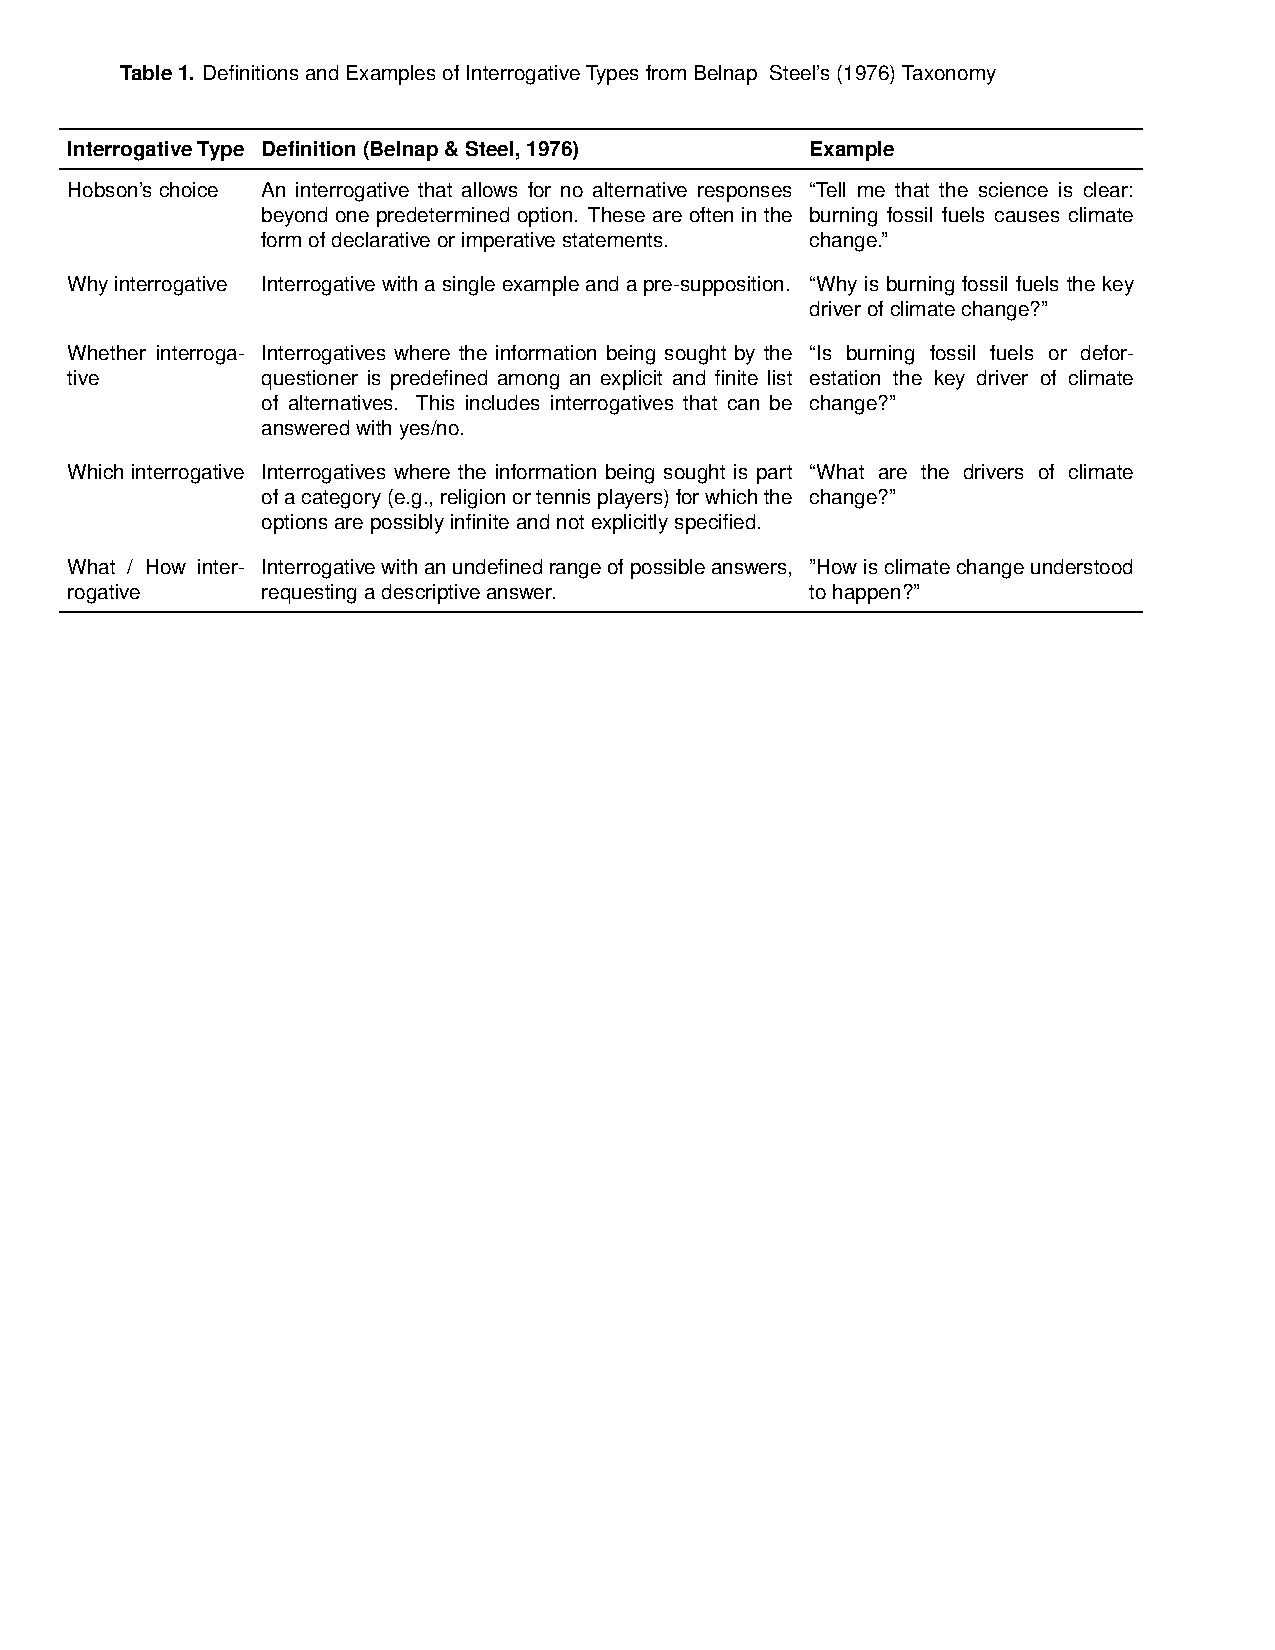
\includegraphics{../03_outputs/01_taxonomies_of_interrogatives/table_1} \end{center}

\subsection{2.2 Data and Methods}\label{data-and-methods}

Ethical approval for the entire research project was obtained via the London School of Economics ethics procedure (reference: 522753). Primary data collection and computational resources for all stages of this research were supported by the LSE Department of Methodology and the Anthropic Student Builders Program. All code and corresponding datasets necessary for replication are publicly available, with full links provided in Appendix A.

\textbf{2.2.1 Dataset Description}

This research draws on Kirk et al.'s (2024) PRISM alignment dataset, which maps the sociodemographic profiles of 1,500 participants from 75 countries to the transcripts of their real conversations with LLMs. Each participant completed a sociodemographic survey prior to engaging in six LLM conversations. To promote prompt diversity, they held two conversations in each of three conditions -- unguided, values-guided, and controversy-guided --, choosing the condition before entering their opening prompt (see §5.2 for discussion of data artefacts). From the conversations, I only include opening prompts in my analyses to avoid confounds introduced by LLM responses. I filtered out non-English entries, to ensure annotator comprehension, resulting in 8,002 prompts from 1,396 participants.

\textbf{2.2.2 Operationalisation} To enable the scalable classification of LLM user prompts, I adopt a computational approach that draws on transformer-based deep learning architectures. This builds on the computational scalability foundational to the logical structure of Belnap and Steel's (1976) taxonomy of interrogatives, leveraging contemporary deep learning methods to enable its scalable application to the analysis of human--language model interactions. While Morucci \& Spirling (\citeproc{ref-morucci_model_2024}{2024}) emphasise the value of simpler generalised linear models in social science, I did not adopt such models because my aim---to capture the \emph{structure}, \emph{purpose}, and \emph{implications} of the prompts---is intrinsically high-dimensional, and a domain where transformer-based architectures offer significant advantages.

Recent research increasingly highlights the significant challenges that transformer-based architectures pose for replicability (\citeproc{ref-barrie_replication_2025}{Barrie et al., 2025}), interpretability (\citeproc{ref-scorzato_reliability_2024}{Scorzato, 2024}), and downstream inference (\citeproc{ref-egami_using_2023}{Egami et al., 2023}) in social scientific applications. I address these concerns both through the fine-grained methodological decisions described throughout this research and in the design of my operationalisation. As part of that design, rather than using a single transformer-based model to predict the interrogative types described in Table 1 directly, I used separate transformer-based models to represent the underlying concepts that Belnap and Steel (1976) define to derive their definitions. I then combined their outputs using Boolean operators according to Belnap and Steel's (1976) definitions to produce the final prompt classifications. This compositional approach enhances interpretability and theoretical alignment by explicitly implementing Belnap and Steel's (1976) definitions into the structure of the classification pipeline. A tool designed to illustrate how this operationalisation works in practice and to examine its limitations, \emph{QuestionTheTaxonomy}, is available \href{https://huggingface.co/spaces/carowagner/questionthetaxonomy}{here} (see Appendix A for full link).

\textbf{2.2.3 Data Labelling}

To develop the data annotation guidelines, I implemented a prescriptive approach (\citeproc{ref-rottger_two_2022-1}{Röttger et al., 2022}) that discourages annotator subjectivity and encourages consistent operationalisation. I decomposed the concepts to be operationalised into their simplest form, as simple and clear annotation instructions have been shown to yield higher-quality labels (\citeproc{ref-laux_improving_2023-1}{Laux et al., 2023}). This resulted in the definition of seven distinct annotation categories, each requiring a dedicated transformer-based classifier, as described in Table 2. Then, I test-annotated a randomly selected sample of 80 prompts to understand edge cases, devise clear descriptions for handling them, and illustrate each guideline with concrete examples from the PRISM dataset (see Appendix B for the full annotator guidelines).

To ensure sufficient class representation for fine-tuning, I proceeded to label 10\% of the dataset (\emph{N} = 800 prompts) for each of the seven annotation categories. To assess inter-coder reliabilities, two annotators labelled a randomly selected 1\% of the dataset (\emph{N} = 80 prompts). As shown in Table 2, inter-annotator agreement was moderate for three categories. To address this, I manually reviewed the disagreements, consulted with the annotators, and refined the annotation guidelines accordingly. Using the improved guidelines, I then relabelled the 10\% of prompts and one annotator relabelled the 1\% of prompts for the three unsatisfactory categories. Second-round reliabilities increased slightly, but indicate potential for further guideline refinement.

\begin{center}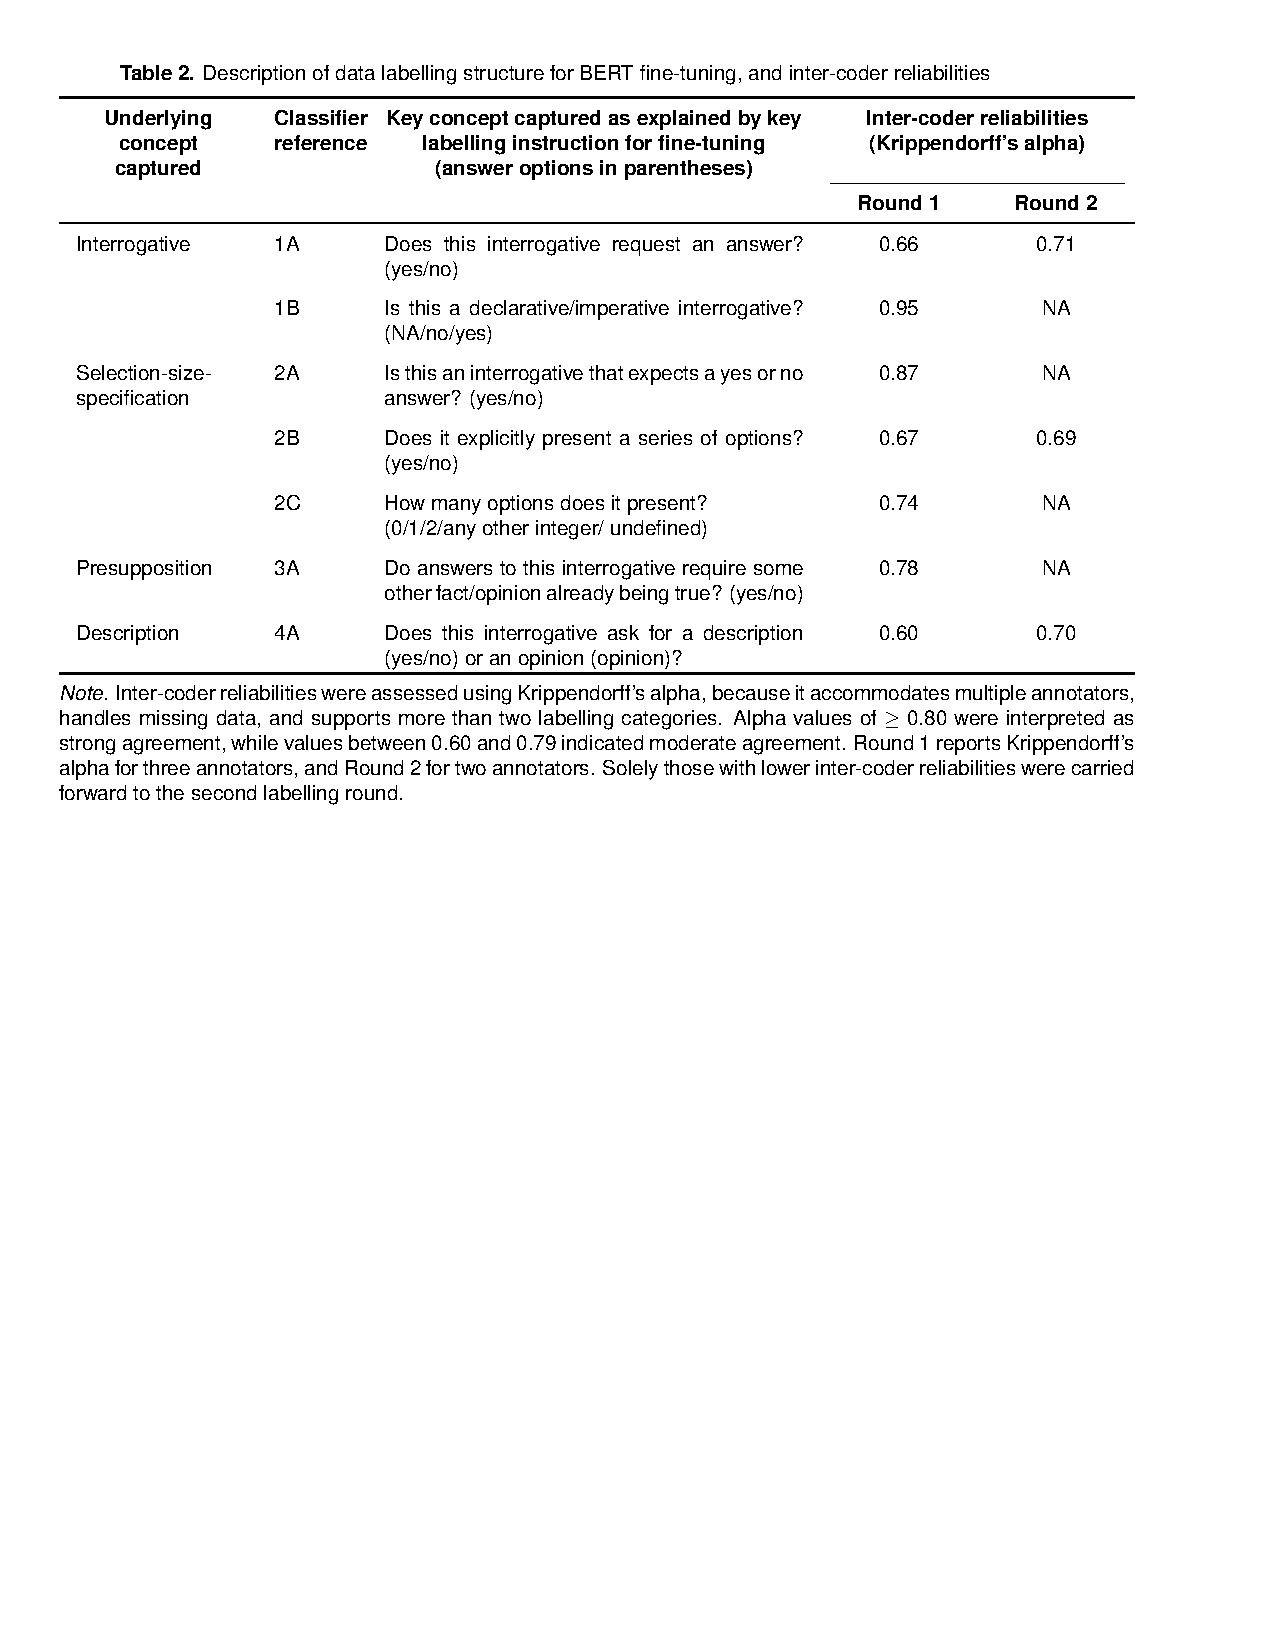
\includegraphics{../03_outputs/01_taxonomies_of_interrogatives/table_2} \end{center}

\textbf{2.2.4 Transformer-based Classifier Selection}

To determine the most suitable classification strategy for operationalising the taxonomy at scale, I tested three approaches using the labelled data: (1) zero-shot prompting based on the human annotation guidelines, (2) few-shot prompting adding labelled examples, and (3) fine-tuning models with transformer-based architectures on the labelled data. In approaches (1) and (2), classification performances were sensitive to prompt formulation; identical prompts performed inconsistently across models, and minor changes in instruction wording led to unpredictable variance. These issues, combined with growing concerns about the replicability of findings when using proprietary or version-dependent generative language models for large-scale annotation (Barrie et al., 2024), led me to focus on approach (3).

In this context, fine-tuning a generative language model, such as Deepseek or those offered by OpenAI, would have required the computational and data resources necessary to update a significant number of parameters that are not relevant to the text-classification task at hand. For this reason, I fine-tuned BERT-based models, which have empirically been shown to be particularly suited for classification tasks (\citeproc{ref-devlin_bert_2018-1}{Devlin et al., 2018}). BERT architectures are open source, can be run locally on most modern hardware, and contain significantly fewer parameters, making them efficient for fine-tuning.

\textbf{2.2.5 BERT Fine-tuning}

Seven separate BERT models were fine-tuned (\citeproc{ref-devlin_bert_2018-1}{Devlin et al., 2018}), one for each classification task described in Table 2, using the Hugging Face transformers library. Each model was trained on 500 labelled prompts from the PRISM dataset, and performance was evaluated on 300 labelled prompts. Fine-tuning was carried out using Hugging Face AutoTrain Advanced on a cloud instance with an Nvidia T4 GPU (16 GB VRAM). Further details on fine-tuning parameters are provided in Appendix C. A key advantage of this approach is that it allowed me to make each model publicly available as a model card on Hugging Face, facilitating future use, and enabling what Barrie et al.~(2024) term stochastic replication, wherein replication results remain reproducible within quantifiable bounds. The outputs of the fine-tuned BERT classifiers were then passed through a set of logical operators described in Table 3 to determine the final interrogative category assignment.

\begin{center}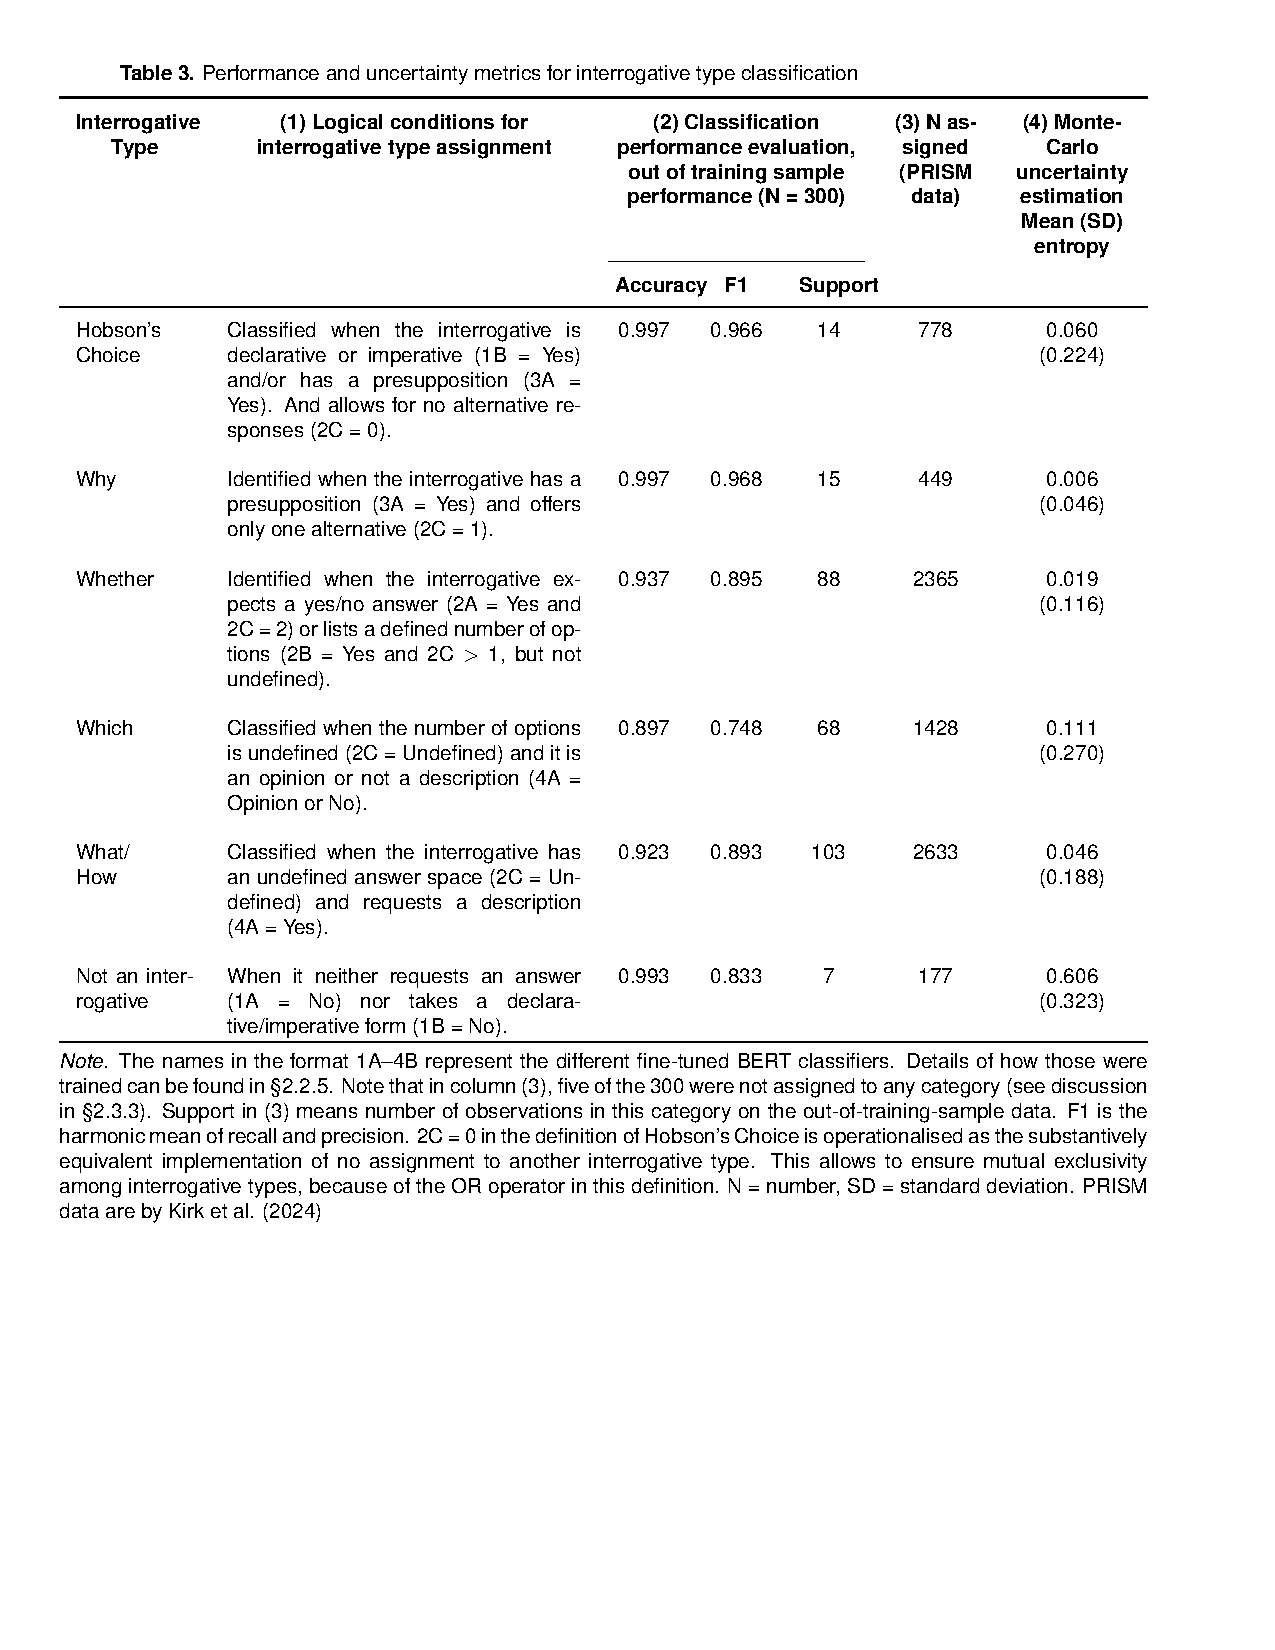
\includegraphics{../03_outputs/01_taxonomies_of_interrogatives/table_3} \end{center}

\clearpage

\subsection{2.3 Results}\label{results}

To examine the robustness of the operationalised taxonomy, I implement a three-part evaluation: (§1) assess classification performance and uncertainty; (§2) evaluate key assumptions underpinning the application of the taxonomy --- namely, that its use generalises beyond the fine-tuning data, that the labels are accurate, and that confidence scores reliably reflect classification performance --- through both quantitative and qualitative approaches; and (§3) consider the implications of these assumptions for inference in social scientific applications.

\textbf{2.3.1 Classification Performance}

Understanding classification performance requires evaluating both the performance of the individual fine-tuned BERT classifiers and how this performance propagates through the logical conditions to produce final classifications. On 300 PRISM user prompts not used during fine-tuning, the accuracies of the seven fine-tuned BERT classifiers ranged between .86-.98 (mean = .94, \emph{SD} = .045) and weighted F1 scores ranged between .85-.98 (mean = .94, \emph{SD} = .050). This indicates robust performance, with accuracy reflecting the overall correctness of predictions, and weighted F1 providing assurance that this performance is not driven solely by dominant categories, as it accounts for both precision and recall per category and adjusts for category prevalence. Notably, the categories with lower classification performance are those that appeared less frequently in the training data. Performances per fine-tuned BERT and category are reported in Appendix D.

When the outputs of the fine-tuned BERT classifiers are passed through the Boolean operators to generate final interrogative category assignments, classification accuracy remains high (range = .896--.997; mean (\emph{SD}) = .957 (.044)), while the weighted F1 score shows a modest decrease (range = .748--.968; mean (\emph{SD}) = .884 (.084)). This drop reflects the compounding of classification uncertainty through the Boolean pipeline, particularly for less frequent categories. Nonetheless, the overall performance remains high, suggesting that the operationalisation is robust even when assigning final interrogative categories. Table 3 reports detailed performances per interrogative type and the number of assigned prompts to each interrogative category across the entire PRISM dataset (columns 3 \& 4).

\textbf{2.3.2 Uncertainty Estimation}

Estimating uncertainty in transformer-based architectures is challenging, not only because it arises from both model-related (epistemic) and data-related (aleatoric) sources (\citeproc{ref-huang_survey_2024}{Huang et al., 2024}; \citeproc{ref-wang_aleatoric_2025}{Wang et al., 2025}), but also because there are limited established standard for its quantitative evaluation (\citeproc{ref-gawlikowski_survey_2022}{Gawlikowski et al., 2022}). I implemented Monte Carlo dropout to estimate epistemic uncertainty, given its compatibility with transformer-based architectures and its computational feasibility for fine-tuned BERT architectures. This method estimates uncertainty by generating multiple stochastic forward passes during inference, each with a different subset of model weights randomly deactivated and computing the variance across the resulting predictions (\citeproc{ref-gal_dropout_2016}{Gal \& Ghahramani, 2016}). For each fine-tuned BERT, I implemented Monte Carlo dropout using a dropout probability of 0.1, as this aligns with standard BERT configurations and falls within the range evaluated by Gal \& Ghahramani (\citeproc{ref-gal_dropout_2016}{2016}). Uncertainty estimates were derived from 100 stochastic forward passes, computed on an Nvidia A100 GPU. Given discrete classes, I calculated interrogative class entropy for each PRISM user prompt across 100 Monte Carlo dropout estimations to quantify epistemic uncertainty. Mean interrogative category-level entropies are reported in Table 3 (column 3), with Why interrogatives eliciting the most certain classifications (mean = 0.006, SD = 0.046) and `Not an interrogative' the least (mean = 0.606, SD = 0.323). Results showed that 91.5\% of the 8'002 PRISM user prompts received the same classification in at least 95 out of 100 Monte Carlo samples. See Appendix E for entropy means and standard deviations of the individual BERT classifiers, and Appendix F for violin plots illustrating the distribution of Monte Carlo entropy across interrogative categories. Taken together, these findings indicate low epistemic uncertainty and high predictive confidence across the majority of the PRISM dataset. This, in turn, supports the reliability of this operationalisation of Belnap and Steel's (1976) taxonomy of interrogatives.

\textbf{2.3.3 Key Assumptions for Taxonomy Application}

Before applying this taxonomy of interrogatives to investigate human--language model interactions, its generalisability must be evaluated, given evidence that fine-tuned BERT models often reflect dataset-specific biases, and that out-of-sample performance may overestimate real-world effectiveness (\citeproc{ref-shen_experimental_2023}{Shen \& Kejriwal, 2023}; \citeproc{ref-de_vassimon_manela_stereotype_2021}{Vassimon Manela et al., 2021}). On the one hand, the PRISM dataset offers a valuable opportunity to address concerns around generalisability, given the diverse backgrounds of its participants. On the other hand, the data originate from a structured academic study in which users were guided toward specific conversation types, which may have introduced data artefacts into the operationalisation (discussed in §5.2).

The meaningful interpretation of downstream inferences depends on the accuracy of the labels in the fine-tuning dataset. This was partly assessed through inter-coder reliabilities, though it should be noted that all annotators were European and held university degrees. Their relative homogeneity may have biased these estimates upward. In addition, while the categories are mutually exclusive, 172 of the 8,002 PRISM user prompts were not assigned to any category, indicating that the classifications were not collectively exhaustive. This is despite the taxonomy being theoretically defined and operationalised to meet both criteria and highlights a gap between the taxonomy's theoretical aims and its empirical implementation. To understand this gap, I manually reviewed the 172 non-assigned prompts. Of those, 13.4\% were not written in English, reflecting limitations in the preprocessing step, which relied on an existing PRISM dataset column for language identification. In addition, some of them had simple statements (e.g., `the titanic') or grammatical mistakes such as `im broed' instead of \emph{I'm bored} -- which should have been assigned to `Not an interrogative', reflecting that this was the category with the fewest labelling examples, and the highest prediction uncertainty. While these cases highlight room for refinement, their 2.8\% incidence across the 8'002 PRISM participant prompts suggests minimal impact on the broader applicability of the taxonomy.

In addition, confidence scores warrant attention as the BERTs' measure of certainty (i.e., softmax output) is frequently treated as a probability, but this assumes the model is well-calibrated---an assumption that does not consistently hold in practice (\citeproc{ref-guo_calibration_2017}{Guo et al., 2017}). Poor calibration arises when the model's softmax output is not adjusted to reflect real-world correctness. In classification, low uncertainty often aligns with a dominant class probability, indicating high confidence; however, high confidence alone does not guarantee low uncertainty, as class probability distribution plays a key role (\citeproc{ref-huang_survey_2024}{Huang et al., 2024}). I evaluated calibration using the Expected Calibration Error, which ranged from 0.93 to 0.99 across fine-tuned BERT classifiers, indicating likely credibility of confidence estimates in applied settings (\citeproc{ref-pavlovic_understanding_2025}{Pavlovic, 2025}).

\textbf{2.3.4 Implications for Inference in Social Scientific Applications}

Understanding robustness involves recognising the operationalisation as an inferential tool for analysing human--language model interactions through a theoretical lens. Egami et al.~(2023) caution that prediction errors from transformer-based classifiers often correlate with both observed and unobserved covariates, thereby introducing dependencies that can substantively distort inferential outcomes. They show that even with high classification accuracy, failing to account for such dependencies can lead to invalid statistical inference. To address this, Egami et al. (\citeproc{ref-egami_using_2023}{2023}) propose the design-based supervised learning (DSL) estimation framework. Given the potential for such bias in BERT-based models, the implementation of the DSL estimator should be treated as integral to this operationalisation. The methods in Study 1 demonstrate how this is applied in practice.

Overall, the above evaluations support the robustness of the operationalisation and its validity for social scientific inference. The taxonomy may serve as a theoretical lens for investigating human--language model interactions, an analysis that can be broken down into two core inquiries: whether user characteristics are associated with interrogative types (Study 1) and whether these types influence LLM responses (Study 2).

\section{3. Study 1 - Descriptive}\label{study-1---descriptive}

\subsection{3.1 Introduction}\label{introduction-1}

This study applies the operationalised taxonomy of interrogatives to characterise variation in Belnap and Steel's (1976) interrogative types by PRISM participant demographic features. Although the present research examines this variation in the broader context of potential human--language model interaction cycles, describing individual variation in the types of interrogatives humans pose in language model interactions is a valuable social scientific pursuit in its own right. This is because language models have the potential to considerably change information retrieval (\citeproc{ref-chen_spiral_2024}{X. Chen et al., 2024}) and production (\citeproc{ref-brachman_current_2025}{Brachman et al., 2025}) --- a shift likely to have broad societal implications (\citeproc{ref-tamkin_understanding_2021}{Tamkin et al., 2021}; \citeproc{ref-weidinger_ethical_2021}{Weidinger et al., 2021}). In this context, my aim to comprehensively describe interrogative types with respect to demographic characteristics may help identify emerging patterns that require further explanation and theorisation (de Kadt \& Grzymala-Busse, 2025).

Given the breadth of inquiry into demographic differences among the types of interrogatives used, I begin this review by focusing on educational background as a key example. Existing literature suggests that higher levels of formal education are associated with the use of more complex \emph{syntactic} structures (\citeproc{ref-massing_degrees_2017}{Massing \& Schneider, 2017}) and \emph{semantically} richer formulations (\citeproc{ref-pereira_language_2022}{Pereira \& Ortiz, 2022}). In addition, differences in educational attainment have been linked to the contexts in which language models are used, which shape the \emph{pragmatic} functions of user prompts (\citeproc{ref-zheng_grice_2021}{Zheng et al., 2021}). Taken together, these patterns in \emph{syntax}, \emph{semantics}, and \emph{pragmatics} suggest corresponding variation in the structure, purpose, and implications of language use by educational background. Since these are the core dimensions captured by Belnap and Steel's (1976) taxonomy of interrogatives, educational attainment emerges as a conceptually relevant variable for describing demographic differences in the use of interrogative types.

More broadly, research drawing on Gricean maxims suggests that demographic characteristics are associated with systematic variation in interactional patterns. For example, Tran (\citeproc{ref-tran_investigation_2020}{2020}) observe conditional differences in the use of Gricean maxims by gender, while Panzeri \& Foppolo (\citeproc{ref-panzeri_childrens_2021}{2021}) do so for age. While these findings offer preliminary indications of potential demographic variation in interrogative type use, they primarily underscore the paucity of empirical research directly characterising such variation in the context of LLM use. In light of this gap---and given the absence of prior empirical applications of Belnap and Steel's (1976) taxonomy in this domain---I implement a broad, descriptive approach. To do so, I draw on the PRISM dataset (\citeproc{ref-kirk_prism_2024}{Kirk et al., 2024}), which includes demographic profiles and opening prompts submitted to large language models, classified according to the operationalised taxonomy of interrogatives.

Adopting the framework for `Good Description' defined by de Kadt \& Grzymala-Busse (\citeproc{ref-good_description_ddk_agb_2025}{2025}) and given a definition of interrogative types (§2.1.3), I define the descriptive scope of my approach as threefold. Let \(d\) denote a demographic characteristic in \{educational status, gender, age, birth region, ethnicity, religion\} or conversation type, \(i\) an interrogative type in \{Hobson's choice, Why, Which, Whether, What/How\}, and \(g\) a subgroup within \(d\). I pose the following research questions:

\begin{adjustwidth}{2em}{2em}
\setlength{\parindent}{0em}%
(1) \textbf{Characteristic}: How frequently does each interrogative type \(i\) occur overall and within each demographic subgroup \(g\)?  

(2) \textbf{Association}: Are individuals in demographic subgroup \(g\) over- or under-represented in asking interrogative type \(i\), relative to their baseline proportion in the PRISM participant sample?  

(3) \textbf{Conditional association}: For each interrogative type \(i\), to what extent is the likelihood of producing that type associated with membership in demographic subgroup \(g\) of feature \(d\), controlling for all other explanatory variables?
\end{adjustwidth}

It is important to approach the interpretation of such observations with caution. Any associations observed between demographic characteristics and interrogative types should not be taken to suggest that the demographic attributes themselves determine how individuals formulate interrogatives. For example, if a gender-related difference is observed, this should not be interpreted as evidence of an inherent distinction between two genders in interrogative patterns. Rather, such findings should be understood as starting points for further inquiry, aimed at uncovering potential social, cultural, or contextual factors that may contribute to the observed variation.

\subsection{3.2 Methods}\label{methods}

This study was pre-registered on OSF, with the full link and a pre-registration accountability statement provided in Appendix G. The methodological substance and the presentation of results draw on Study 1 by Kirk et al.~(2024, pp.6-7). In this study, I carry forward the PRISM conversation opening prompts that I classified according to the operationalised taxonomy of interrogatives by Belnap \& Steel (\citeproc{ref-belnap_logic_1976}{1976}) in the preceding section. I analyse these prompts in conjunction with demographic data from the PRISM participant profiles (see Kirk et al. (\citeproc{ref-kirk_prism_2024}{2024}) for details). The 172 PRISM opening prompts not assigned to any interrogative category were excluded from the present analyses.

Since the DSL R package (\citeproc{ref-egami_dsl_2025}{Egami et al., 2025}) does not yet support all analytical strategies, the implementation of the DSL estimator was adapted to suit the specific requirements of each analysis and is described in the corresponding sections. In general, I treated the seven fine-tuned BERT classifiers and the logical conditions for final category assignment as an ensemble, both to account for error propagation through the full classification process and because the final interrogative category is the outcome of inferential interest. Given the nominal nature of the interrogative categories and to preserve interpretability, I created a dummy-encoded column for each final interrogative category assignment across all PRISM prompts and applied the DSL estimator to each dummy variable separately to generate a debiased estimate for each interrogative category. Extended methods for implementing the DSL estimator across the three sections below are described in Appendix H.

\textbf{3.2.1 Characteristic}

For each demographic feature \(d\), I computed a contingency table to display the joint frequency distribution of interrogative types. This provides an initial overview of the data distribution and allows for the derivation of three types of insights for each demographic variable d and interrogative type \(i\). First, the joint probability of each interrogative type and demographic group \(\Pr(i, d)\), can be calculated. Then, the conditional probability of an interrogative type given a demographic group, \(\Pr(i \mid d)\), and of a demographic group given an interrogative type \(\Pr(d \mid i)\), can also be derived.

To complement the contingency table analyses and assess the robustness of observed patterns, I applied the DSL estimator to adjust for non-random prediction errors in each interrogative category \(i\) and to quantify uncertainty in the estimates. I used the DSL R package (\citeproc{ref-egami_dsl_2025}{Egami et al., 2025}), regressing each dummy-encoded interrogative category \(i\) on each demographic feature d using linear regression without an intercept. This approach is mathematically equivalent to computing subgroup means. Although it is less interpretable, this was necessary because the DSL package (v0.1.0) does not currently support aggregated count data.

\textbf{3.2.2 Association}

For each interrogative type \(i\) and demographic feature \(d\) (e.g., gender), over-representation factors were calculated separately for each subgroup \(g\) within the feature (e.g., women, men, non-binary within the gender feature). These factors assess whether each subgroup is over- or under-represented in asking that interrogative type, relative to its baseline proportion in the overall PRISM sample. This is calculated using the following formula:

\[ 
\text{Over-representation factor}_{g,i} = \frac{\frac{N_{g,i}}{N_i}}{\frac{N_g}{N_{\text{total}}}} 
\]

The numerator represents the \emph{observed prevalence} of demographic subgroup \(g\) (e.g., women within the demographic feature of gender) within interrogative type \(i\). Specifically, \(N_{g,i}\)~is the number of times individual in demographic subgroup asked interrogative type \(i\) and \({N_i}\)~is the total number of times interrogative type \(i\) is asked across all subgroups within that feature. The denominator represents the \emph{expected prevalence} if group g participated proportionally to its prevalence in the data. Thus, \(\frac{N_g}{N_{\text{total}}}\) represents group \(g\)'s baseline rate in the full sample.

To adjust for non-random prediction errors in the interrogative classification, I computed the over-representation factors using design-adjusted outcomes for each dummy-encoded interrogative type. These were implemented manually, as the current version of the DSL package (v0.1.0) does not support this type of analysis.

\textbf{3.2.3 Conditional association}

To estimate the conditional association between demographic characteristics and the likelihood that a prompt is of interrogative type \(i\), I estimate the following specification using a logistic regression for each interrogative category, here \(y^{i}\):

\[
\begin{aligned}
\operatorname{logit}\left(\Pr\left(y^{i}_{p,o} = 1\right)\right)
&= \alpha_i
+ \text{gender}'_{p} \, \beta^{i}_{1}
+ \text{age}'_{p} \, \beta^{i}_{2}
+ \text{birth region}'_{p} \, \beta^{i}_{3} \\
&\quad + \text{religion}'_{p} \, \beta^{i}_{4}
+ \text{prompt type}'_{p} \, \beta^{i}_{5}
+ \text{ethnicity}'_{p} \, \beta^{i}_{6}
+ \varepsilon_{p,o}
\end{aligned}
\]

where \(y_{p,o}^{i}\)~takes the value of 1 if the prompt written by participant \(p\) in opening prompt \(o\) is of interrogative type \(i\). In this context, \(\alpha_{i}\)~is an intercept specific to interrogative type i, \(\beta_{d}^{i}\)~is a coefficient vector for demographic feature \(d\) for interrogative type \(i\), and \(\varepsilon_{p,o}\)~is the error term clustered at the participant level to account for repeated measures, as each participant contributes multiple opening prompts to the dataset. Following the implementation by Kirk et al. (\citeproc{ref-kirk_prism_2024}{2024}), gender, age, region, ethnicity, religion, and conversation type are included in the model as sets of dummy variables. The omitted reference categories are Male, 18--24, United States, White, Not religious, and Unguided. Bonferroni corrections were applied to adjust for multiple comparisons.

A limitation of my implementation is that the results from these logistic regressions are presented without DSL adjustment, as the current version of the DSL R package (Egami et al., 2025) does not support logistic models with clustered standard errors. In this context, the manual implementation described in §3.2.2 is not appropriate because adjusted outcomes are continuous, making them unsuitable as dependent variables in logistic specifications.

\subsection{3.3 Results}\label{results-1}

\textbf{3.3.1 Characteristic}

The contingency tables in panel A of Figure 1 show how frequently each interrogative type occurs overall and within each demographic group. Taken together, the findings indicate that, across demographic variables, participants more frequently used open-ended interrogatives (those with higher \emph{selection-size specifications}), such as What/How, Which, and Whether, compared to closed-ended interrogatives (with lower \emph{selection-size specifications}) like Why and Hobson's Choice. For example, the top-left cell in the gender panel shows 398 Hobson's Choice interrogatives authored by women. From this, it can be derived that 5.4\% of all interrogatives fit this category, that 11.1\% of interrogatives by women were Hobson's Choice, and that 52.8\% of Hobson's Choice interrogatives were from women\footnote{\(\Pr(\text{Hobson’s choice}, \text{female}) = 398 / 7404 \approx \mathbf{5.4\%}\).\\
  Row-wise: \(\Pr(\text{Hobson’s choice} \mid \text{female}) = 398 / 3588 \approx \mathbf{11.1\%}\).\\
  Column-wise: \(\Pr(\text{Female} \mid \text{Hobson’s choice}) = 398 / 753 \approx \mathbf{52.8\%}\).\\
  Note that the latter is influenced by the baseline distribution of demographic groups in the data.}. One notable pattern is that, in conversations on topics that participants considered controversial, they most frequently used more closed-ended interrogatives such as Whether (38.1\%), whereas in unguided conversations on a random topic, open-ended interrogatives like What/How were most common (47.3\%; \(\Pr(\text{interrogative type} \mid \text{conversation type})\)). Appendix I reports DSL-adjusted category proportions along with associated uncertainty estimates. These adjusted values confirm the same substantive patterns observed in the main results.

\begin{center}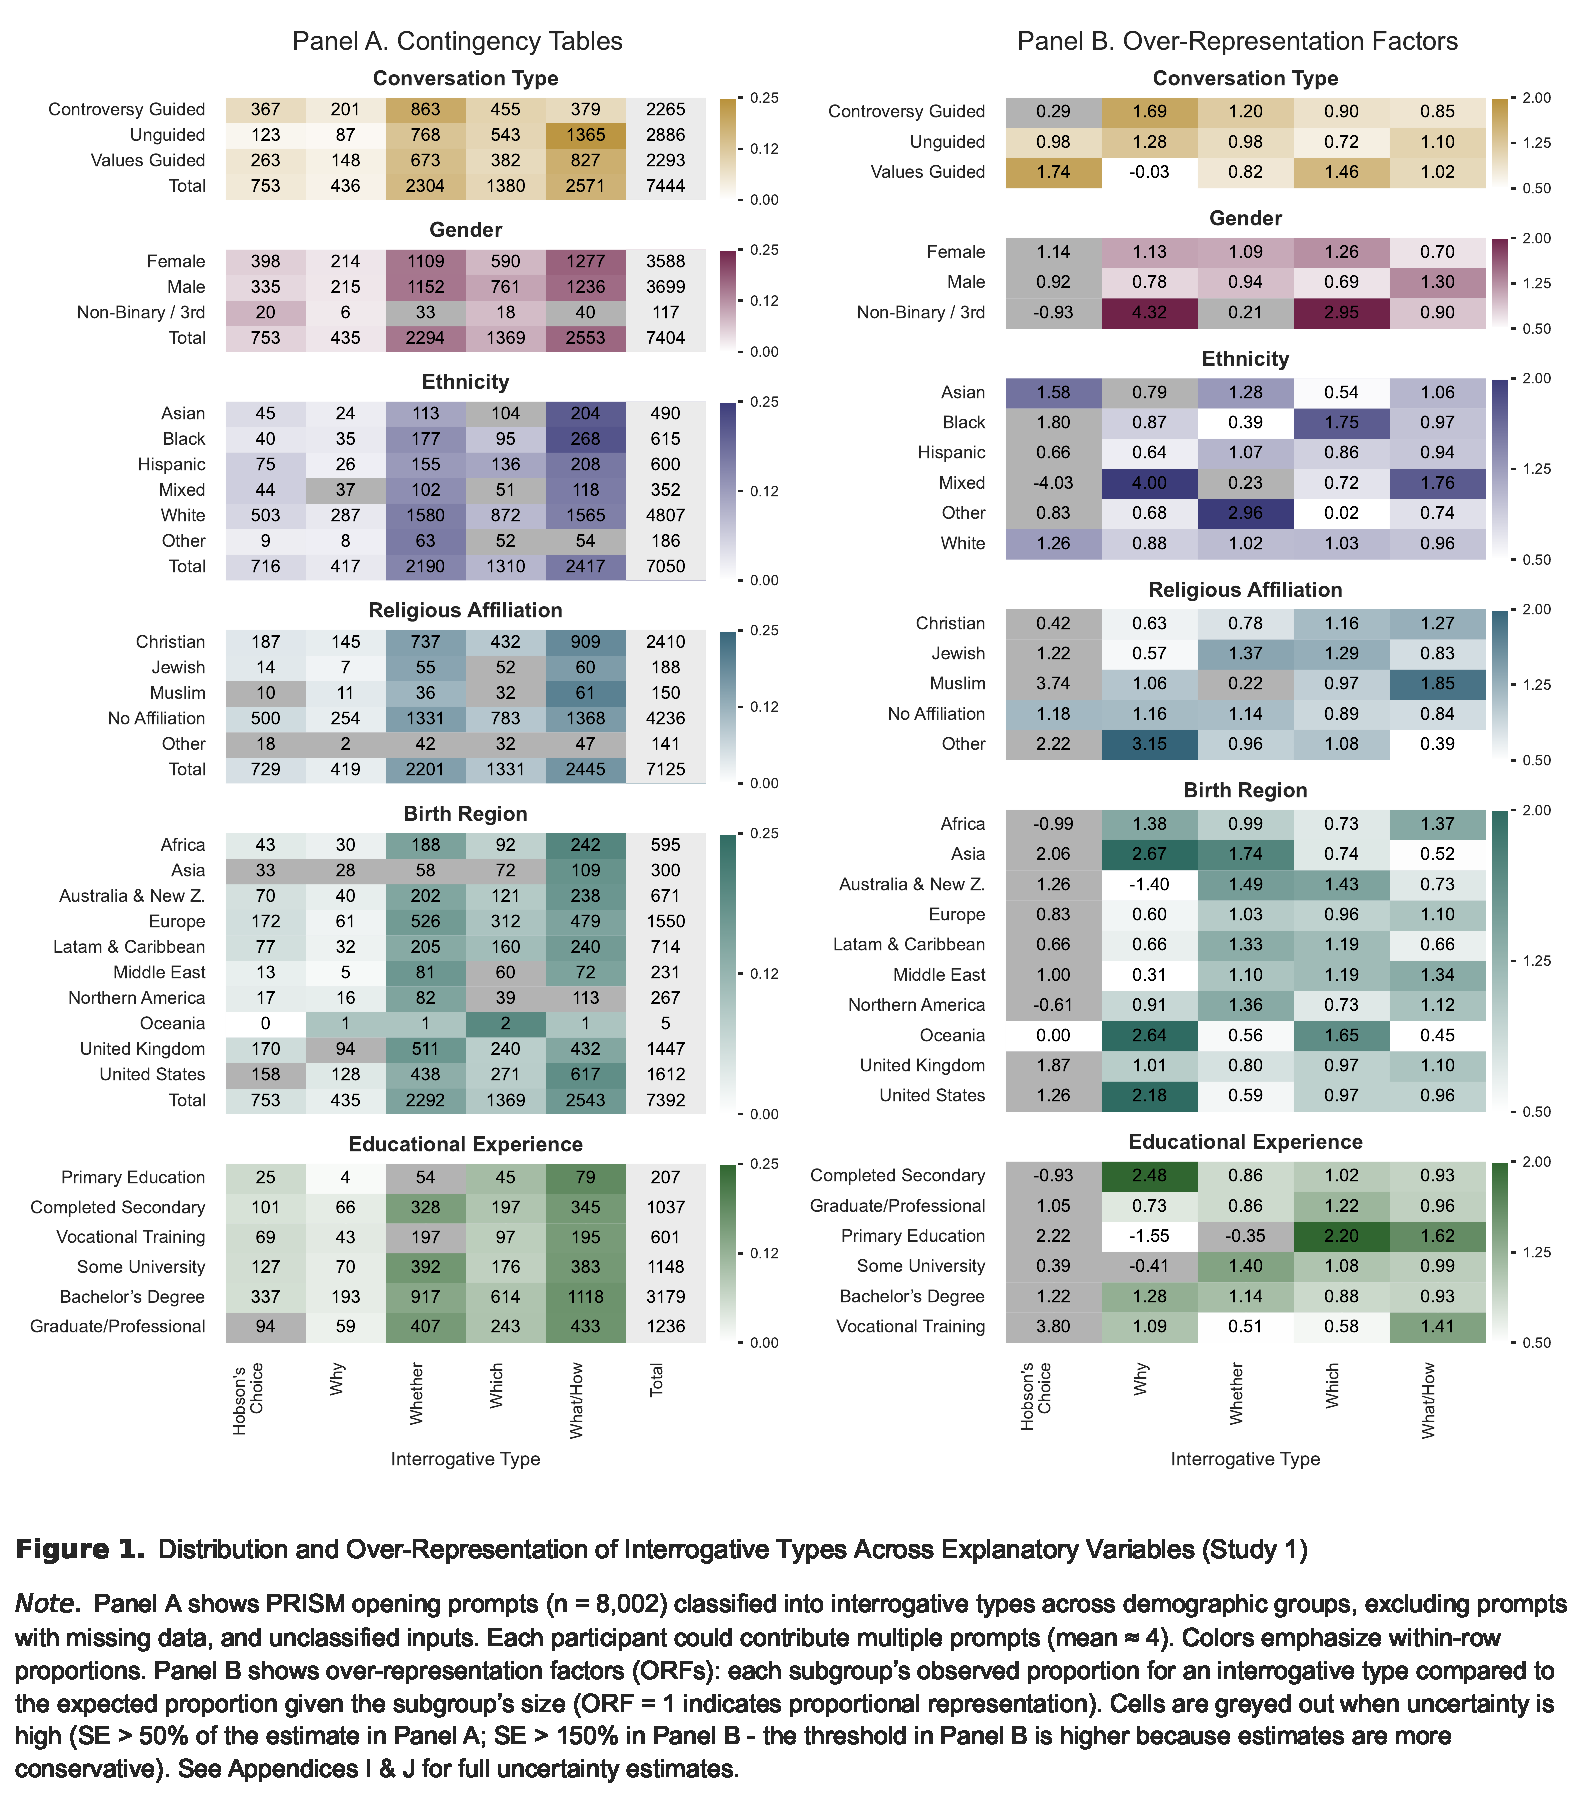
\includegraphics{../03_outputs/02_descriptive_analyses/figure_1} \end{center}

\textbf{3.3.2 Association}

As shown in Panel B of Figure 1, the distribution of over-representation factors adds nuance to the observations derived from contingency tables. Overall, open-ended interrogatives show more stable distributions across demographic groups, with lower uncertainty estimates and more subtle disparities in representation. In contrast, closed-ended interrogatives tend to be more unevenly distributed across subgroups, as reflected in a wider range of over-representation factors and higher uncertainty estimates. To illustrate, in the birth region panel, over-representation factors for What/How interrogatives range from 0.45 to 1.37, whereas for Hobson's Choice they span a wider range, from --0.99 to 2.06. Uncertainty estimates reflect the underlying data distribution, with lower-frequency interrogatives showing greater variability (see Appendix J for full estimates). As an example, participants with completed secondary education make up 13.9\% of the sample but account for just 12.9\% of What/How interrogatives, yielding an over-representation factor of 0.93 (\emph{SE} = 0.10).

\textbf{3.3.3 Conditional association}

Figure 2 presents results from a series of logistic regression specifications, each estimating how the odds of using a given interrogative type vary across demographic subgroups, relative to an omitted reference group, controlling for all other demographic features. These results suggest that, \emph{ceteris paribus}, participants aged 18--24 were more likely to use closed-ended Why interrogatives and less likely to use open-ended Which interrogatives compared to all older age groups. Average marginal effects, presented in panel B of Figure 2, indicate that, controlling for other demographic characteristics, participants aged 18--24 were on average 3.2 percentage points (pp) more likely to ask a Why interrogative than those aged 25--34, and 6.0 pp more likely than those aged 55--64. In contrast, their likelihood of using Which interrogatives was 4.8 pp lower than those aged 25--34, and 11.6 pp lower than those aged 55--64.

Similar patterns were observed for education and conversation type. Participants with only primary and/or some secondary education were more likely to use closed-ended Why and Whether interrogatives and less likely to use open-ended Which and What/How forms compared to all higher levels of educational attainment, \emph{ceteris paribus}, although these associations were not found to be statistically significant. Conversation type showed the largest effect size. When discussing a topic they perceived as controversial, in reference to a randomly selected topic, participants were 11.6 pp more likely to use the most closed-ended interrogative form (Hobson's Choice) and 28.5 pp less likely to use the most open-ended form (What/How) controlling for other demographic characteristics. Patterns for ethnicity, religion, and birth region were more heterogeneous (see Appendix K for predicted probabilities).

\begin{center}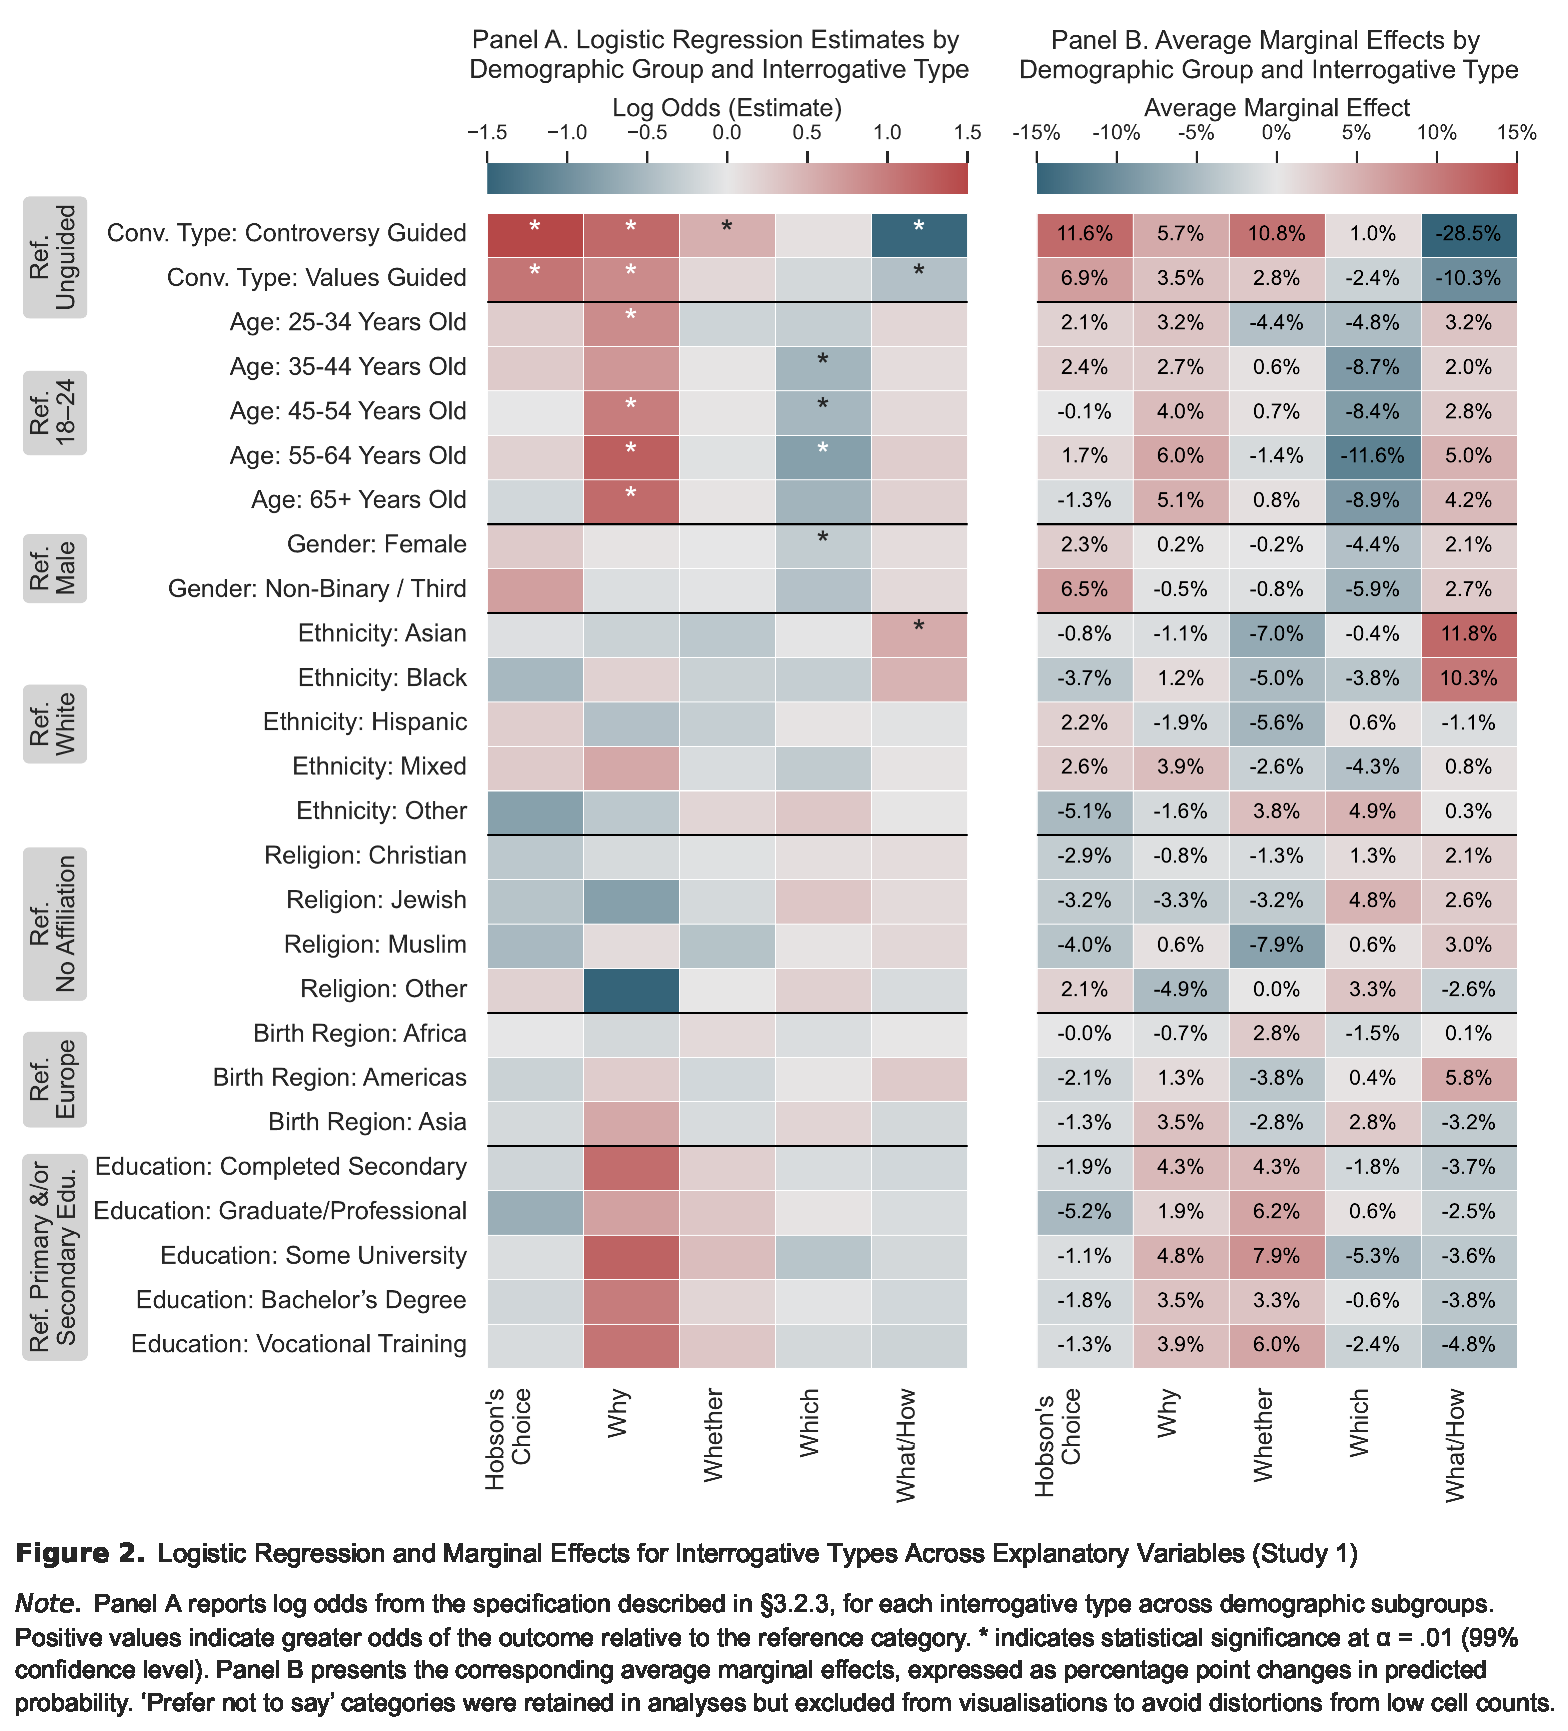
\includegraphics{../03_outputs/02_descriptive_analyses/figure_2} \end{center}

To conclude, the observations described in this study suggest that the types of interrogatives posed, as categorized by Belnap and Steel (1976), do vary with individuals' demographic characteristics, with the most pronounced patterns observed in relation to educational attainment, age, and conversation type. The analyses were linked to theory through the use of Belnap \& Steel (\citeproc{ref-belnap_logic_1976}{1976}) ~taxonomy of interrogatives, operationalised in an open-source manner. This transparency facilitates future testing and comparison, while the use of universal demographic characteristics provides anchor points for interpretation across social scientific disciplines. In combining these, I sought to produce descriptions that are clear, comparable, and complete (de Kadt \& Grzymala-Busse, 2025). The described patterns provide starting points for further inquiry into how individual differences in the widespread use of LLMs across the world may be shaping practices of information retrieval and production (discussed in §5.2).

\section{Study 2 - Experimental}\label{study-2---experimental}

\subsection{4.1 Introduction}\label{introduction-2}

In this study, I experimentally manipulate interrogative form by comparing the most open-ended type (What/How), as defined by the operationalised taxonomy, with the most closed-ended form (Hobson's Choice), to evaluate whether they lead to differences in language model response attributes. These attributes are measured using the Google Jigsaw bridging attributes---which include affinity, compassion, curiosity, nuance, personal story, reasoning, and respect (\citeproc{ref-lees_new_2022}{Lees et al., 2022})---as they were specifically developed to assess communicative qualities associated with constructive and prosocial dialogue (\citeproc{ref-ovadya_bridging_2023}{Ovadya \& Thorburn, 2023}). While there is a large body of research on how prompt differences influence LLM responses, it primarily approaches the topic either from an engineering perspective, focused on optimising model function, or from a methodological perspective, aimed at augmenting social scientific research methods. However, most research does not consider that everyday users may be inadvertently engaging in a form of prompt engineering through individual differences in their routine interactions with LLMs, as described in Study 1. As a result, there remains a significant gap in the literature concerning potential variation in LLM responses among everyday users, and the broader social scientific implications of such differences. In this study, my aim is to take a first step toward addressing this gap by examining how interrogative form may influence language model response attributes associated with constructive online dialogue.

A growing body of prompt engineering literature has emerged in response to the sensitivity of language models to input phrasing, aiming primarily to optimise model performance. In a systematic review, Schulhoff et al. (\citeproc{ref-schulhoff_prompt_2025}{2025}) identify 58 distinct prompting techniques, reflecting the multidimensionality of prompt design. One such technique, instruction selection (\citeproc{ref-jiang_how_2020}{Jiang et al., 2020}), manipulates the \emph{syntactic} form of prompts while preserving their underlying meaning. Aimed at optimising LLM knowledge evaluation, their study demonstrates that the effectiveness of eliciting latent model knowledge in responses varies substantially with prompt \emph{syntax}, even when meaning is held constant. Press et al. (\citeproc{ref-press_measuring_2023}{2023}) developed Self-Ask, a prompting technique that explicitly refines the original prompt by generating clarifying sub-questions. This process manipulates the prompt's \emph{semantic} structure by making implicit presuppositions and implications explicit, which in turn leads to systematic changes in language model responses, particularly in performance on compositional reasoning tasks. Prompt \emph{pragmatics} are manipulated by Li et al. (\citeproc{ref-li_large_2023}{2023}) through their emotion prompting technique. By embedding affective statements such as `This is very important to my career' the technique alters the contextual framing of the prompt, thereby influencing LLM responses across a range of benchmarking tasks.

Several studies have adopted a more social scientific approach, focusing on the sociocultural implications of prompt variation in contrast to the engineering emphasis on optimising model performance. For example, Viveros-Muñoz et al. (\citeproc{ref-viveros-munoz_does_2025}{2025}) found that \emph{syntactic} differences affected students' perceived response quality; Kharchenko et al. (\citeproc{ref-kharchenko_how_2025}{2025}) demonstrated that \emph{semantic} framing based on cultural values led to heterogeneity in LLM response attributes; and Yin et al. (\citeproc{ref-yin_should_2024}{2024}) showed that prompt politeness influenced responses through \emph{pragmatic} framing. Together, the findings stemming from both approaches described above suggest differences in language model response attributes according to \emph{syntactic}, \emph{semantic}, and \emph{pragmatic} variation in input prompts. Since these dimensions are central to Belnap and Steel's (1976) taxonomy of interrogatives, their taxonomy may offer a theoretically grounded lens through which to investigate whether variation in interrogative type corresponds with differences in language model response attributes. Overall, this lends itself to the following research question:

\begin{adjustwidth}{2em}{2em}
How does the use of Hobson’s Choice prompts, relative to What/How prompts, influence the expression of the Google Jigsaw bridging attributes in LLM-generated responses?
\end{adjustwidth}

Understanding the potential association between interrogative form and LLM response attributes is particularly relevant in applied contexts where LLMs can influence decision-making (e.g., medical, or organisational settings), as it may affect how users interpret, trust, or act on LLM responses.

\subsection{4.2 Methods}\label{methods-1}

This study was pre-registered on OSF (see Appendix G for full link and accountability statement). To examine the effects of interrogative form on LLM responses, I selected prompts from the PRISM dataset that were classified as What/How and Hobson's Choice according to the operationalised taxonomy (Belnap \& Steel, 1976) and constructed counterfactuals in the opposite form. I then collected LLM responses and analysed variation in the responses' bridging attributes.

\textbf{4.2.1 Study Design}

\emph{Experimental manipulation.} To meet the requirement of 400 prompt pairs from pre-registered power calculations, I randomly selected 250 PRISM opening prompts classified as Hobson's Choice and 250 as What/How, based on the operationalised taxonomy of interrogatives, and constructed counterfactuals for each in the opposite interrogative form. Oversampling allowed to preserve statistical power after manually verifying and removing misclassified prompts. I then reviewed the selected prompts to identify recurring formulations within each interrogative type and, in conjunction with Belnap and Steel's definitions and illustrative examples, developed five distinct prompt templates per type to account for LLM prompt sensitivity. The full set of templates, along with example implementations, are provided in Appendix L. Each selected PRISM prompt was then randomly assigned a counterfactual template from the opposite interrogative category, and the corresponding counterfactual was manually written to ensure alignment with the Belnap and Steel's (1976) interrogative definitions.

For example, one PRISM participant asked, ``What happens if we achieve AGI?'' Using the first Hobson's Choice template (\emph{Tell me that X}), this was rephrased as ``Tell me the benefit of achieving AGI.'' By definition, such transformations required increased specificity and imposed a particular evaluative framing on the prompt content. To ensure variation, I deliberately alternated between framings; for instance, the prompt ``what is google adsense?'' was rephrased as ``Tell me the disadvantage of google adsense.'' However, the heterogeneity of the PRISM prompts prevented me from implementing a fully algorithmic framing across all cases. For example, a prompt such as ``What is the best actress?'' does not naturally map onto an advantage/disadvantage formulation within the \emph{Tell me that X} template and thus required case-by-case judgment to generate a counterfactual consistent with the definitions provided by Belnap \& Steel (\citeproc{ref-belnap_logic_1976}{1976}). As a result, a limitation of this study is that counterfactual phrasings may reflect the subjective choices of a single annotator.

\emph{Data collection and processing.} In response to concerns that empirical findings may not replicate across LLM architectures (Barrie et al., 2024), I submitted both original PRISM and counterfactual prompts to a diverse set of commercial LLMs and collected their responses. LLMs were selected to represent a cross-section of current architectures, varying in both scale (i.e., relatively small vs.~large parameter counts) and intended reasoning capacity (reasoning vs.~non-reasoning). Across major providers---Anthropic, DeepSeek, Google, Meta, Microsoft, MistralAI, OpenAI, and Qwen---I aimed to include one LLM per category. Where such distinctions were unavailable for a given provider, selection followed pre-registered criteria. This yielded a final sample of 21 LLMs, each accessed via provider APIs (full LLM versions and provider details in Appendix M). All LLMs were queried using default parameters to approximate typical user interactions. In downstream analyses, intermediate reasoning traces (`thinking tokens') were excluded from reasoning LLM outputs to reflect the final user-facing response. To determine token length and ensure consistent token number comparisons across LLMs, all responses were tokenised using the GPT-4 tokeniser from the tiktoken library. I then evaluated all LLM responses using the Google Jigsaw Perspective API (\citeproc{ref-lees_new_2022}{Lees et al., 2022}), which produced scores for the bridging attributes outlined in Table 4. I chose the Google Jigsaw bridging attributes because they were specifically developed to evaluate communicative qualities that support constructive and prosocial dialogue in human interactions in accordance with Ovadya \& Thorburn (\citeproc{ref-ovadya_bridging_2023}{2023}). Understanding whether interrogative form leads to variation in these attributes within LLM outputs may offer insight into how such systems can shape, support, or constrain meaningful interaction in everyday use.

\begin{center}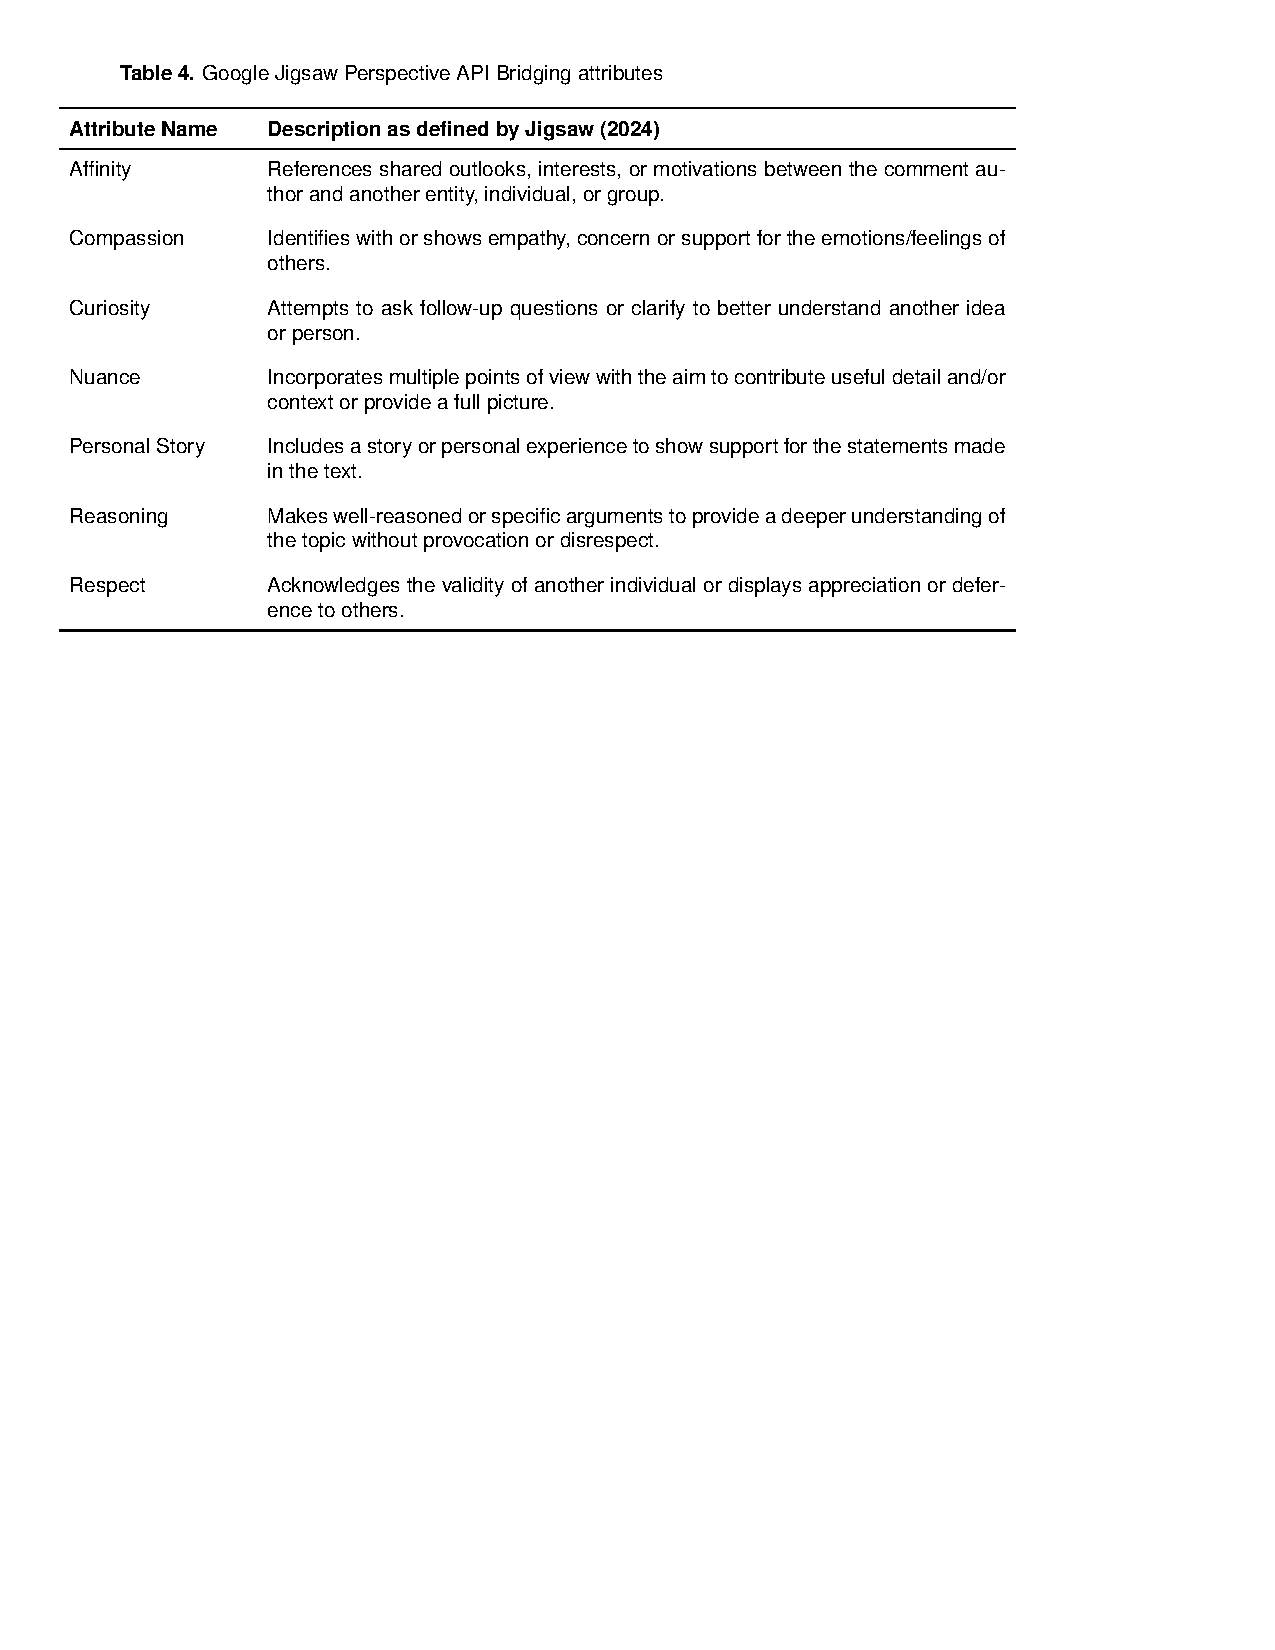
\includegraphics{../03_outputs/03_experimental_analyses/table_4} \end{center}

\textbf{4.2.2 Analytical Strategy}

I start by comparing LLM response lengths in terms of token number between Hobson's Choice and What/How prompts using paired \emph{t}-tests and Cohen's \emph{d}, both overall and by LLM. To qualitatively evaluate whether and how interrogative structure shapes response content, I conduct a structured comparison using outputs from OpenAI as a case study, selected for being the most widely used provider in the sample. I randomly select 50 prompt pairs and their corresponding responses from GPT-4 and O4, OpenAI's most used reasoning and non-reasoning LLMs, and manually evaluate them in relation to the three following key theoretical attributes identified by Belnap and Steel (1976): \emph{selection-size-specification}, \emph{presupposition}, and \emph{completeness-claim-specification}.

Then, I estimate the average treatment effect as the difference in means of response scores between the two interrogative types across each of the seven Jigsaw bridging attributes, both for each LLM and in the full sample. For each of these comparisons, I assess whether attribute variance differs between response types by implementing Levene's test.

To estimate the effect of the interrogative type experimental manipulation on the bridging response attributes of LLM responses, I implement the following specification:

\[
\begin{aligned}
\text{AttributeScore}_{ij} &= \alpha
+ \beta_{1} \, \text{InterrogativeType}_{i}
+ \beta_{2} \, \text{LLM}_{j} \\
&\quad + \beta_{3} \left( \text{InterrogativeType}_{i} \times \text{LLM}_{j} \right)
+ \varepsilon_{ij}
\end{aligned}
\]

Where \(\text{AttributeScore}_{ij}\) denotes the score assigned to LLM \(j\)'s response to prompt \(i\) on one of the seven Google Jigsaw bridging attributes. \(\text{InterrogativeType}_{i}\) is a binary treatment indicator equal to 1 if the prompt is a What/How interrogative and 0 if it is a Hobson's Choice prompt (the reference category). \(\text{LLM}_{j}\) is a categorical variable indicating LLM identity, included as a series of dummy variables with GPT-4.1 as the reference level. The interaction term, \(\text{InterrogativeType}_{i}\times\text{LLM}_{j}\), captures LLM-specific differences in responsiveness to interrogative form. The error term, \(\varepsilon_{ij}\), is clustered at the prompt level to account for repeated measurements across LLMs for the same prompt. To facilitate interpretation, I computed marginal effects of interrogative type by LLM for each bridging attribute, using predictions from the above specification and applying parametric Monte Carlo simulations (1,000 draws) to derive uncertainty estimates via the \texttt{marginaleffects} R package (\citeproc{ref-arelbundock_interpret_2024}{Arel-Bundock et al., 2024}).

\clearpage

\subsection{4.3 Results}\label{results-2}

\textbf{4.3.1 Descriptive}

An analysis of response length across the 17,984 collected responses indicated that LLM responses to What/How interrogatives were substantially longer than those to Hobson's Choice prompts, but that effect sizes varied by LLM. The mean (\emph{SD}) number of tokens for What/How prompts was 568.16 (406.31), compared to 394.12 (315.76) for Hobson's Choice. A paired-samples t-test confirmed this difference, \emph{t}(8991) = 47.10, \emph{p} \textless{} .001, with a medium effect size (Cohen's \emph{d} = 0.50). As shown in Appendix N, this is consistent with the pattern observed for 19 of the 21 LLMs, Mistral Magistral Medium and DeepSeek R1 being the exceptions, suggesting that the aggregate difference is unlikely to be an artefact of Simpson's paradox but it's magnitude should still be interpreted with caution (\citeproc{ref-pearl_understanding_2013}{Pearl, 2013}). The magnitude of the effect varied between individual LLMs, with 11 LLMs having a Cohen's \emph{d} above 0.8, 6 below 0.6, and the remainder in-between.

\textbf{4.3.2 Qualitative}

For closed-ended prompts, responses often referred to options outside the predefined answer space (\emph{selection-size-specification}) and the \emph{presupposition}, typically by asking the user whether additional information was desired without explicitly specifying that information. In contrast, responses to What/How prompts tended to present a structured overview of possible options, frequently concluding with summary statements. Nearly all responses were formatted as numbered bullet points. While What/How responses were generally longer and more comprehensive, their degree of comprehensiveness appeared to vary. This aligns with Belnap and Steel's (1976) concept of \emph{completeness-claim-specification}, whereby open-ended What/How interrogatives leave it to the respondent to determine what constitutes a satisfactory answer. With the present approach, I was unable to identify the factors underlying variation in comprehensiveness, which therefore remains a question for future research.

\textbf{4.3.3 Quantitative}

Findings from differences-in-means analyses across the full sample suggested meaningful differences between LLM responses to Hobson's Choice prompts and those to What/How prompts across all seven bridging attributes. Specifically, responses to What/How prompts scored, on average, 6.5 percentage points (pp) lower in affinity, 4.8 pp lower in compassion, 3.3 pp lower in curiosity, 4.4 pp lower in personal storytelling, and 4.0 pp lower in respect compared to responses to Hobson's Choice prompts. Conversely, What/How responses scored 3.3 pp higher in nuance and 1.6 pp higher in reasoning than Hobson's Choice responses (all \emph{p}'s \textless{} .001). The direction of effects was largely consistent across individual LLMs, though the magnitude of differences varied. Levene's tests indicated unequal variances between What/How and Hobson's Choice prompts for all attributes (\emph{p} \textless{} .001), except for curiosity (\emph{p} = .756). These results suggest that, on average, bridging attribute scores in LLM responses vary not only in central tendency but also in dispersion, depending on the interrogative form of the prompt. Full results, including average treatment effects and uncertainty estimates for individual LLMs and the full sample, are presented in Appendix O.

As shown in Figure 3, findings from the specification described in §4.2.2 closely mirrored those from the difference-in-means analyses. On average, moving from the LLM response to a Hobson's Choice interrogative, to the LLM response to a What/How interrogative was associated with increases in nuance and reasoning, and decreases in affinity, compassion, curiosity, personal story, and respect. While the direction of effects was broadly consistent across LLMs, their magnitude varied by LLM. Several LLMs exhibited particularly large sensitivity to prompt type (e.g., GPT-4.1, Claude Sonnet 4), whereas others showed attenuated effect sizes (e.g., Mistral Magistral Medium, DeepSeek R1).

For example, for Anthropic's Claude 3 Haiku LLM, moving from a Hobson's Choice prompt to a What/How prompt was associated, on average, with a 10 pp decrease in affinity, 6 pp decrease in compassion, 5 pp decrease in curiosity, 12 pp decrease in personal story and 6 pp decrease in respect while leading to a 3 pp increase in nuance, and a 1 pp increase in reasoning, holding other explanatory variables constant. Full point estimates and confidence intervals are reported in Appendix P. Results were largely consistent in both direction and uncertainty estimates across two alternative specifications: one that included a random intercept for prompt (to account for paired interrogatives), and another that omitted clustered standard errors by prompt type.

\begin{center}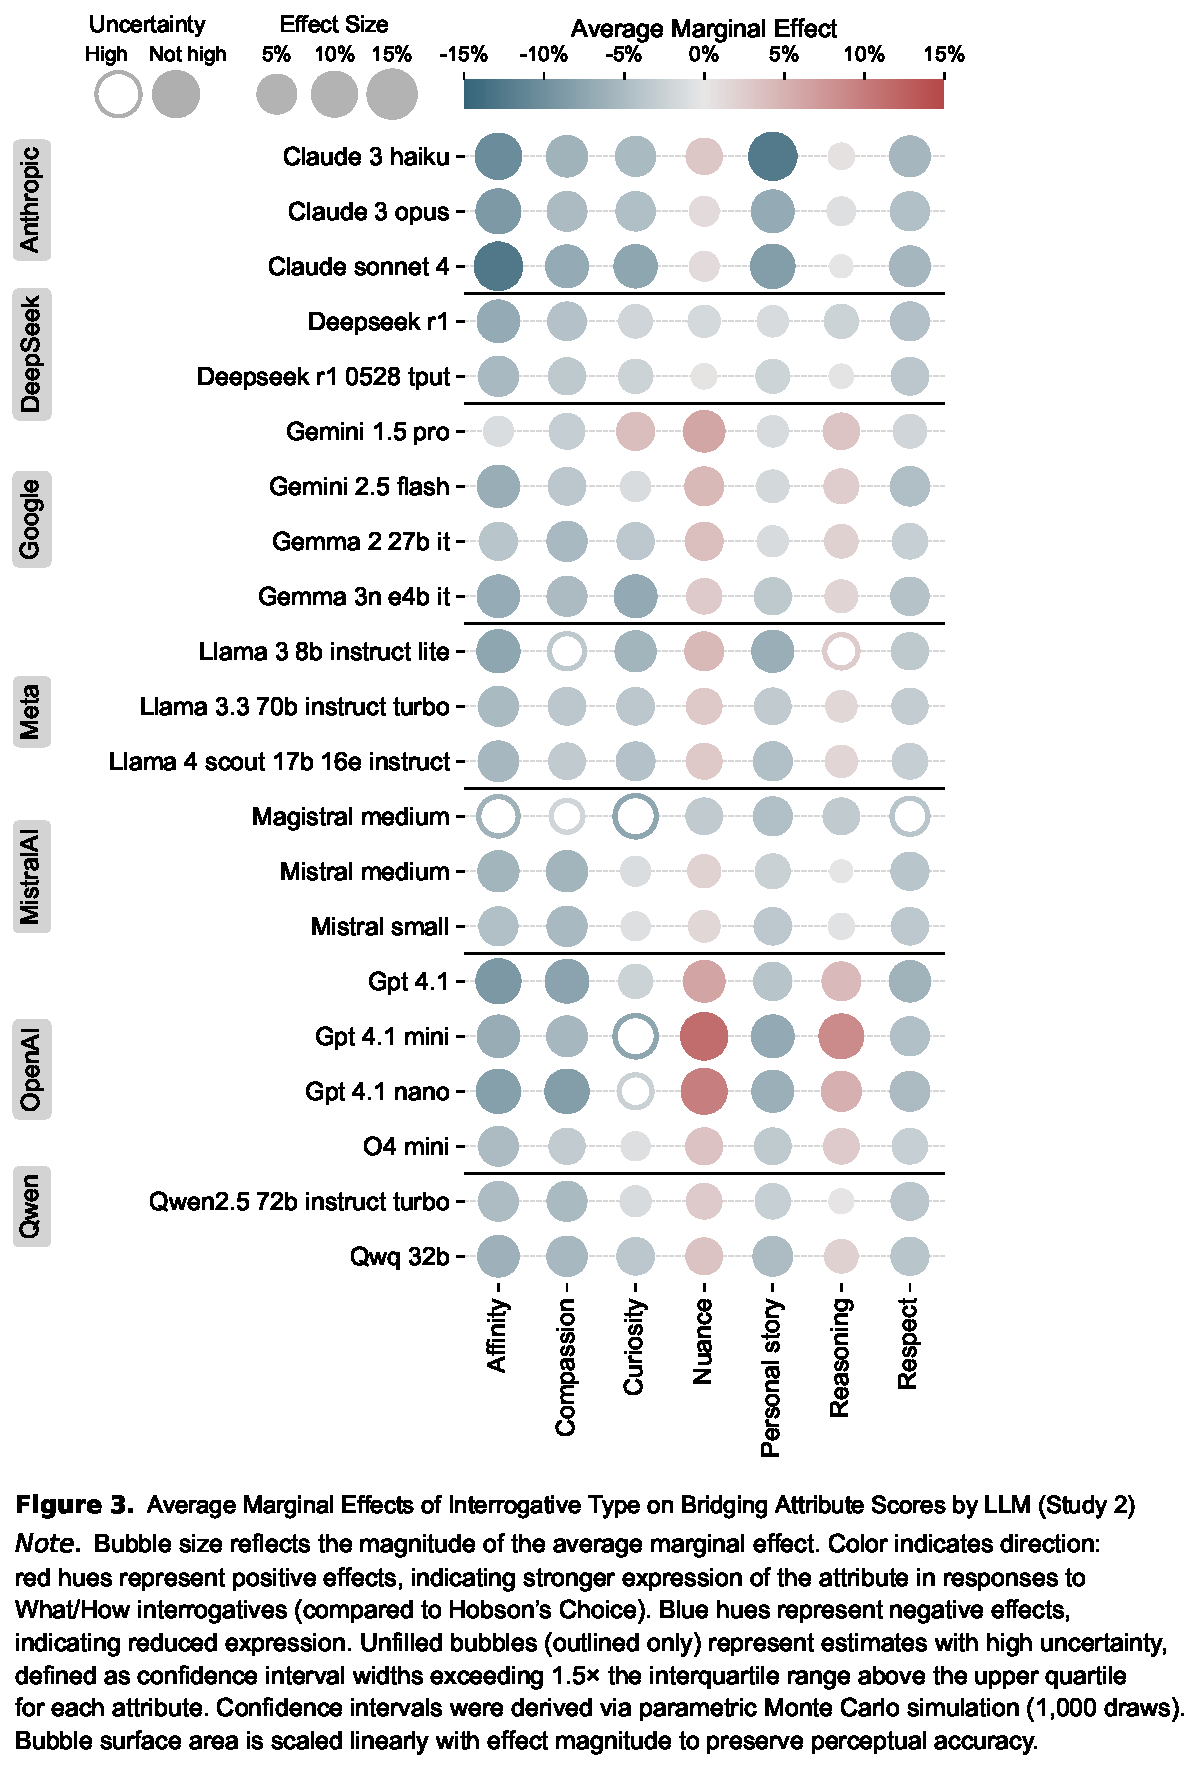
\includegraphics{../03_outputs/03_experimental_analyses/figure_3} \end{center}

Overall, the findings from this experimental study suggest that the interrogative form of prompts influences the expression of bridging attributes in LLM-generated responses. Responses to What/How prompts were generally longer and exhibited greater nuance and reasoning, but consistently lower levels of affinity, compassion, curiosity, personal storytelling, and respect compared to responses to Hobson's Choice prompts. While the direction of effects was broadly consistent across LLMs, their magnitude varied substantially, indicating that LLMs differ in their sensitivity to interrogative framing (see §5.2 for a discussion of implications).

\section{5. Discussion \& Conclusion}\label{discussion-conclusion}

In the context of changes in information retrieval and production associated with the widespread adoption of LLMs, I operationalised Belnap and Steel's (1976) taxonomy of interrogatives. I selected this taxonomy for its ability to avoid the normative constraints of earlier frameworks and its potential to support social scientific research at scales relevant to LLM deployment. Throughout the operationalisation and evaluation, I sought to address concerns regarding replicability, interpretability, and downstream inference. The findings demonstrated high predictive performance and strong reliability, with overall low uncertainty that modestly increased for categories with limited training data. Taken together, results suggest that this operationalisation may hold utility in the social scientific investigation of human--language model interactions.

To this end, findings from the observational Study 1 suggested that closed-ended interrogatives were more likely among younger participants, those with higher educational attainment, as well as in conversations about controversial topics and values, with effect sizes varying across interrogative types and demographic subgroups. The robustness of these observations is supported by the diversity of the sample, comprising 1,396 participants from 75 birth countries, and provides a basis for future research into these associations. In the experimental Study 2, manipulation of interrogative type revealed that, relative to the most open-ended form, the most closed-ended form elicited LLM responses exhibiting greater affinity, compassion, curiosity, personal storytelling, and respect, as well as reduced nuance and reasoning. These directional effects were broadly consistent across 21 LLMs, though their magnitude varied, and the manipulation influenced not only the central tendency of bridging attribute distributions but also their variance.

Together, these findings indicate that cycles of human--language model interactions may emerge, shaped by both user characteristics and LLM-specific properties. More broadly, they highlight that understanding the social scientific implications of the widespread LLM adoption requires moving beyond isolated analyses of either user inputs or LLM outputs towards an integrated, higher-dimensional examination of both.

\textbf{5.1 Limitations}

When evaluating the present operationalisation, both a theoretical and a technical limitation should be noted. Belnap \& Steel (\citeproc{ref-belnap_logic_1976}{1976}) formulated an assertional language of logical expressions to formalise and prove their erotetic logic, from which they derived concepts at the `meta-language level', such as \emph{selection-size-specification}. In this study, I operationalised these concepts, thereby assuming that the foundational assertions of their formal system hold in the applied context. A more granular evaluation of this theoretical alignment with respect to the assertional language was beyond the present scope but should be prioritised in future research. In addition, the study's focus on interrogatives leaves unaddressed the operationalisation of Belnap and Steel's (1976) formalisation of answers, which could further enhance the theory's potential for analysing human--language model interactions. The technical limitation reflects a broader gap in the literature, in that systematically developed guidelines to evaluate construct validity in deep-learning--based operationalisations have not yet been established. While I have sought to address these issues by considering replicability, interpretability, and downstream inference alongside predictive performance and uncertainty quantifications, the absence of standardised validation protocols remains a limitation and constrains the comparability of findings across studies.

A key limitation of Study 1 is that PRISM data may contain artefacts of its academic study context, possibly compromising ecological validity as recorded prompts may diverge from everyday LLM use. Kirk et al. (\citeproc{ref-kirk_prism_2024}{2024}) sought to encourage a more naturalistic LLM-use setting in their study design by leaving input prompt choice as a free parameter; however, future work should evaluate the generalisability of these findings using observational data. This is particularly pertinent to the described associations between conversation type and interrogative type, where unusually large effect sizes warrant careful scrutiny and replication. The case for validating these findings with observational data is reinforced by a second limitation: although the PRISM data are diverse, their reliance on crowd workers introduces the generalisability constraints typical of such samples (Stewart et al., 2017). Participants were active internet users who opted into a specific task for hourly remuneration, potentially shaping both sample composition and engagement.

In study 2, creating Hobson's Choice counterfactuals for What/How interrogatives required greater specificity and imposed a particular evaluative framing on the prompt content. Despite the mitigation measures described in §4.2.1, the heterogeneity of PRISM prompts precluded a fully algorithmic approach. Because the reformulations were produced by a single annotator, potential subjectivity may affect internal validity; this could be improved in future work by incorporating multiple annotators and agreement checks. Similarly, some counterfactuals may be less contextually plausible than the original PRISM prompts, reinforcing the importance of implementing this experimental design with observational data to evaluate the generalisability of findings.

\textbf{5.2 Potential Applications and Future Research}

Given the universality of question-asking and the expansive scope of information represented within LLMs, the social scientific implications---and thus the potential applications---of Belnap and Steel's (1976) theoretical framework are extensive. To illustrate, I discuss two potential applications drawn from distinct domains.

First, such cycles may have important implications in medicine, where research increasingly explores their use to reduce the burden on healthcare practitioners (\citeproc{ref-gaber_evaluating_2025}{Gaber et al., 2025}). From the clinician's perspective, D. Chen et al. (\citeproc{ref-chen_large_2025}{2025}) describe LLM use in assisting with symptom documentation and retrieving information from large patient files. If certain clinicians are more likely to use closed-ended interrogatives when retrieving patient information, and this leads to shorter LLM responses with less nuance and reasoning but greater affinity, repeated exchanges of this kind could create a self-perpetuating cycle that progressively narrows the diagnostic dialogue. In some cases, such narrowing may reduce the likelihood of retrieving rare or unexpected symptoms. Investigating this risk and its potential to introduce new inequalities or exacerbate existing ones in diagnostic quality is an important area for future inquiry.

Similar types of human-LLM interaction cycles may emerge in patient-facing implementations of LLMs. For instance, Chen et al.~(2025) also describe their use as tools to facilitate patient understanding. Examining this potential in future studies is important, as such cycles could be associated with patients under-reporting or over-interpreting symptoms. Taken together, these examples illustrate the range of dynamics that must be considered, underscoring the complexity involved in understanding the potential consequences of widespread LLM integration in healthcare.

Second, constructive dialogue on politically relevant topics among the population is considered a key component of healthy democracies, and its reported decline in the context of rising political polarisation has raised concern (\citeproc{ref-caluwaerts_deliberation_2023}{Caluwaerts et al., 2023}; \citeproc{ref-novoa_generically_2023}{Novoa et al., 2023}). Recent findings indicate that LLMs are increasingly used as sources of information on politically relevant topics, including elections, geopolitical conflicts, or rights-based issues such as abortions (\citeproc{ref-aoki_large_2024}{Aoki, 2024}; \citeproc{ref-zhu_learn_2025}{Zhu et al., 2025}) Findings from the present study suggest a potential pathway that could contribute to reduced constructive dialogue: if the discussion of controversial and values-based topics is more often associated with closed-ended interrogatives (Study 1), and such interrogatives tend to elicit responses with comparatively less reasoning and nuance but greater affinity and compassion (Study 2), this may, in some contexts, limit the scope for constructive exchange. Future research should examine how such cycles of human--LLM interaction influence the conditions associated with constructive dialogue, including their potential role as a pathway for (mis)belief acquisition.

To conclude, I operationalised Belnap and Steel's (1976) taxonomy of interrogatives as a theoretical lens to investigate the potential consequences of the rapid, widespread adoption of LLMs. In doing so, I sought to address the gap in the literature concerning how everyday users may inadvertently engage in prompt engineering through individual differences in their routine LLM interactions, and the implications for response characteristics. Findings from two studies applying this operationalisation indicated potential cycles in human--LLM interactions, shaped by both user characteristics and LLM-specific properties. These emphasise the need for future research across different domains of application to understand their potential consequences and inform timely safeguards.

\clearpage

\section{6. Appendices}\label{appendices}

\begin{center}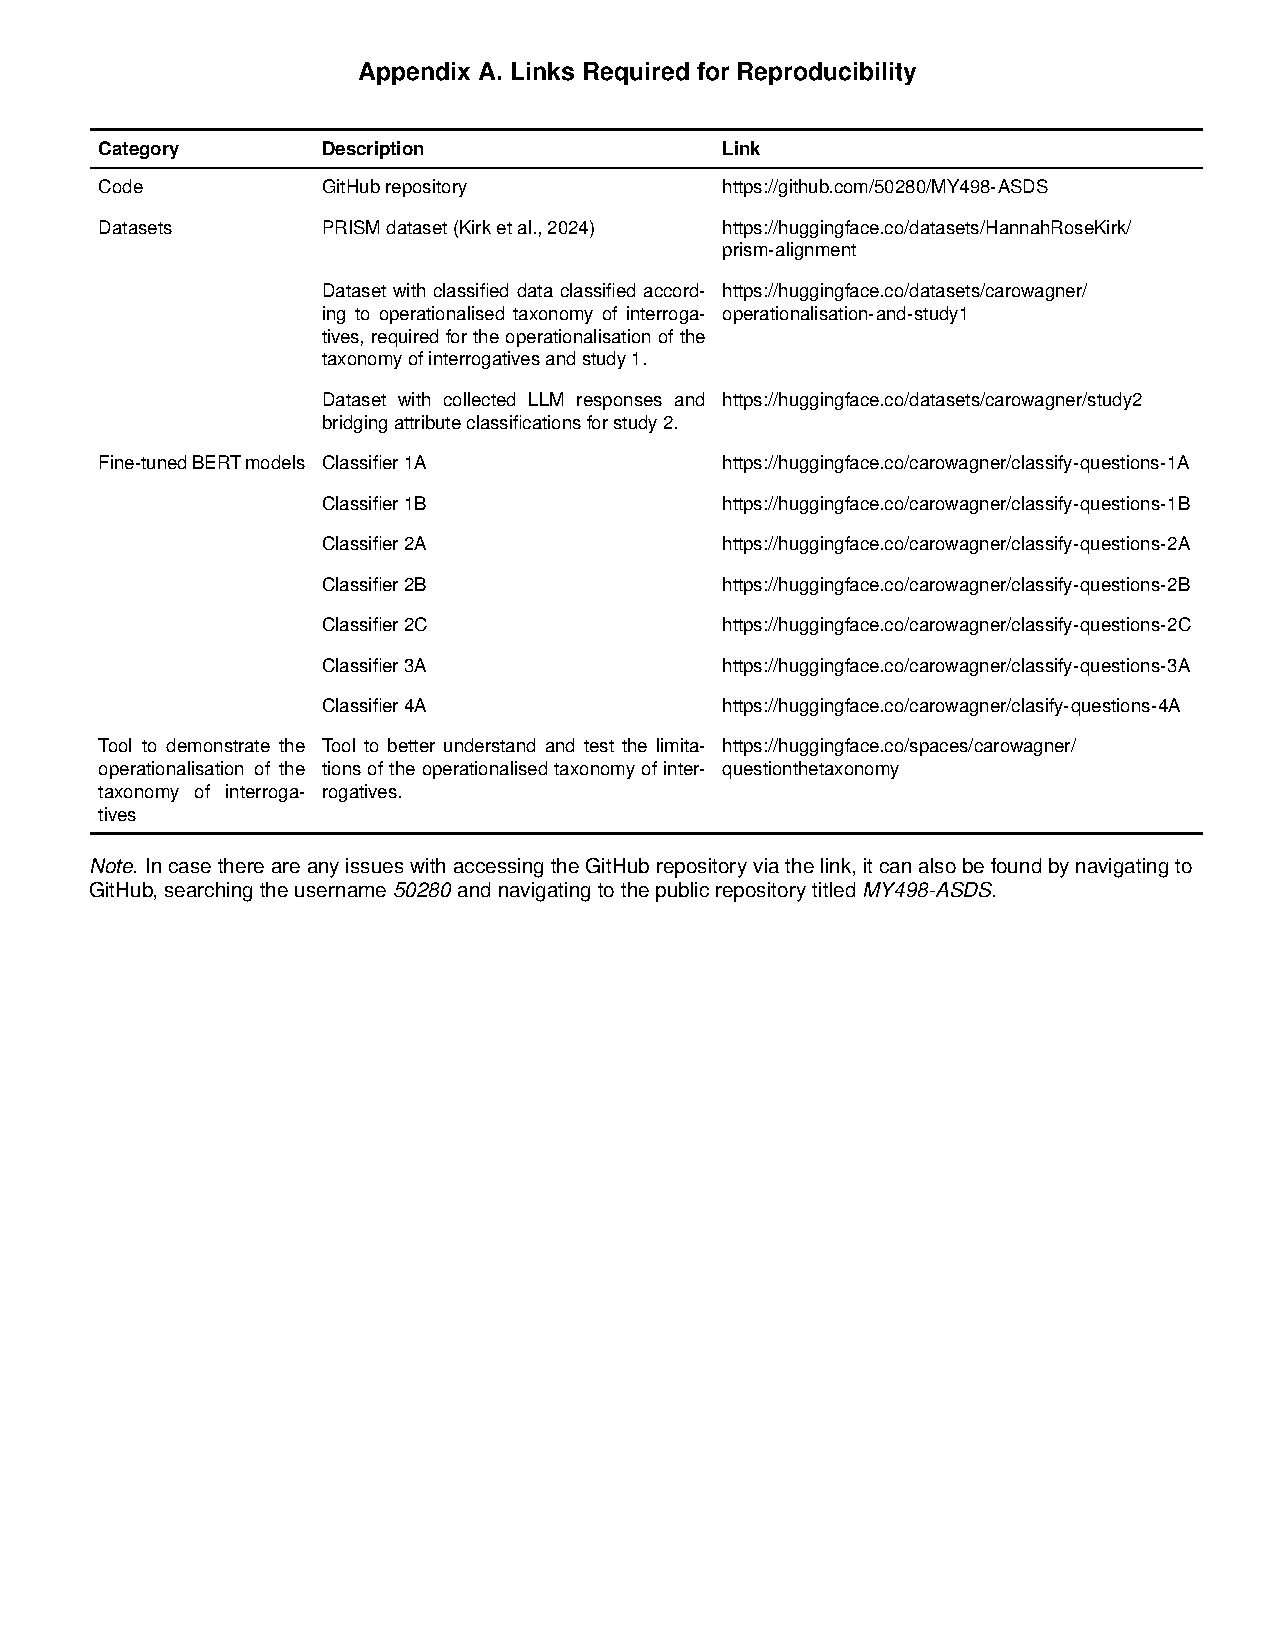
\includegraphics{../03_outputs/04_appendices/appendix_a} \end{center}

\begin{center}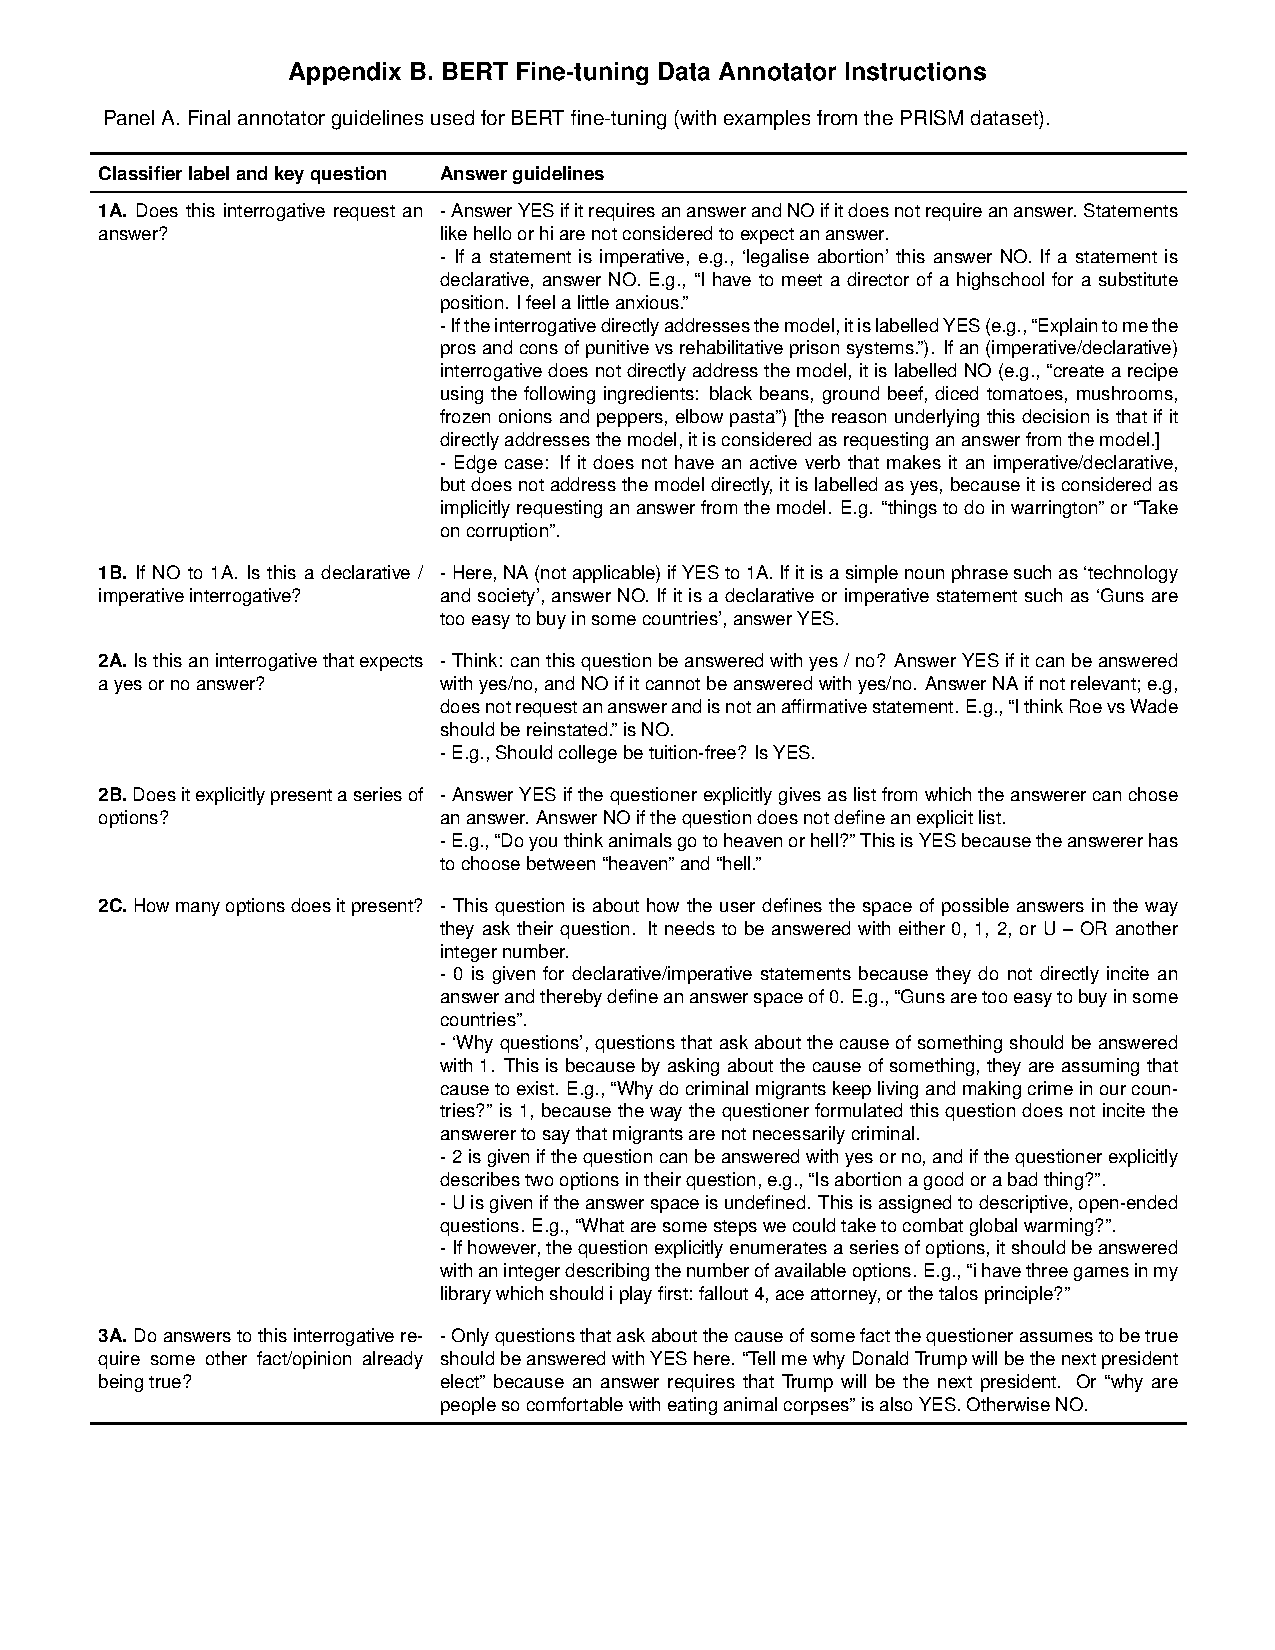
\includegraphics{../03_outputs/04_appendices/appendix_b_i} \end{center}

\begin{center}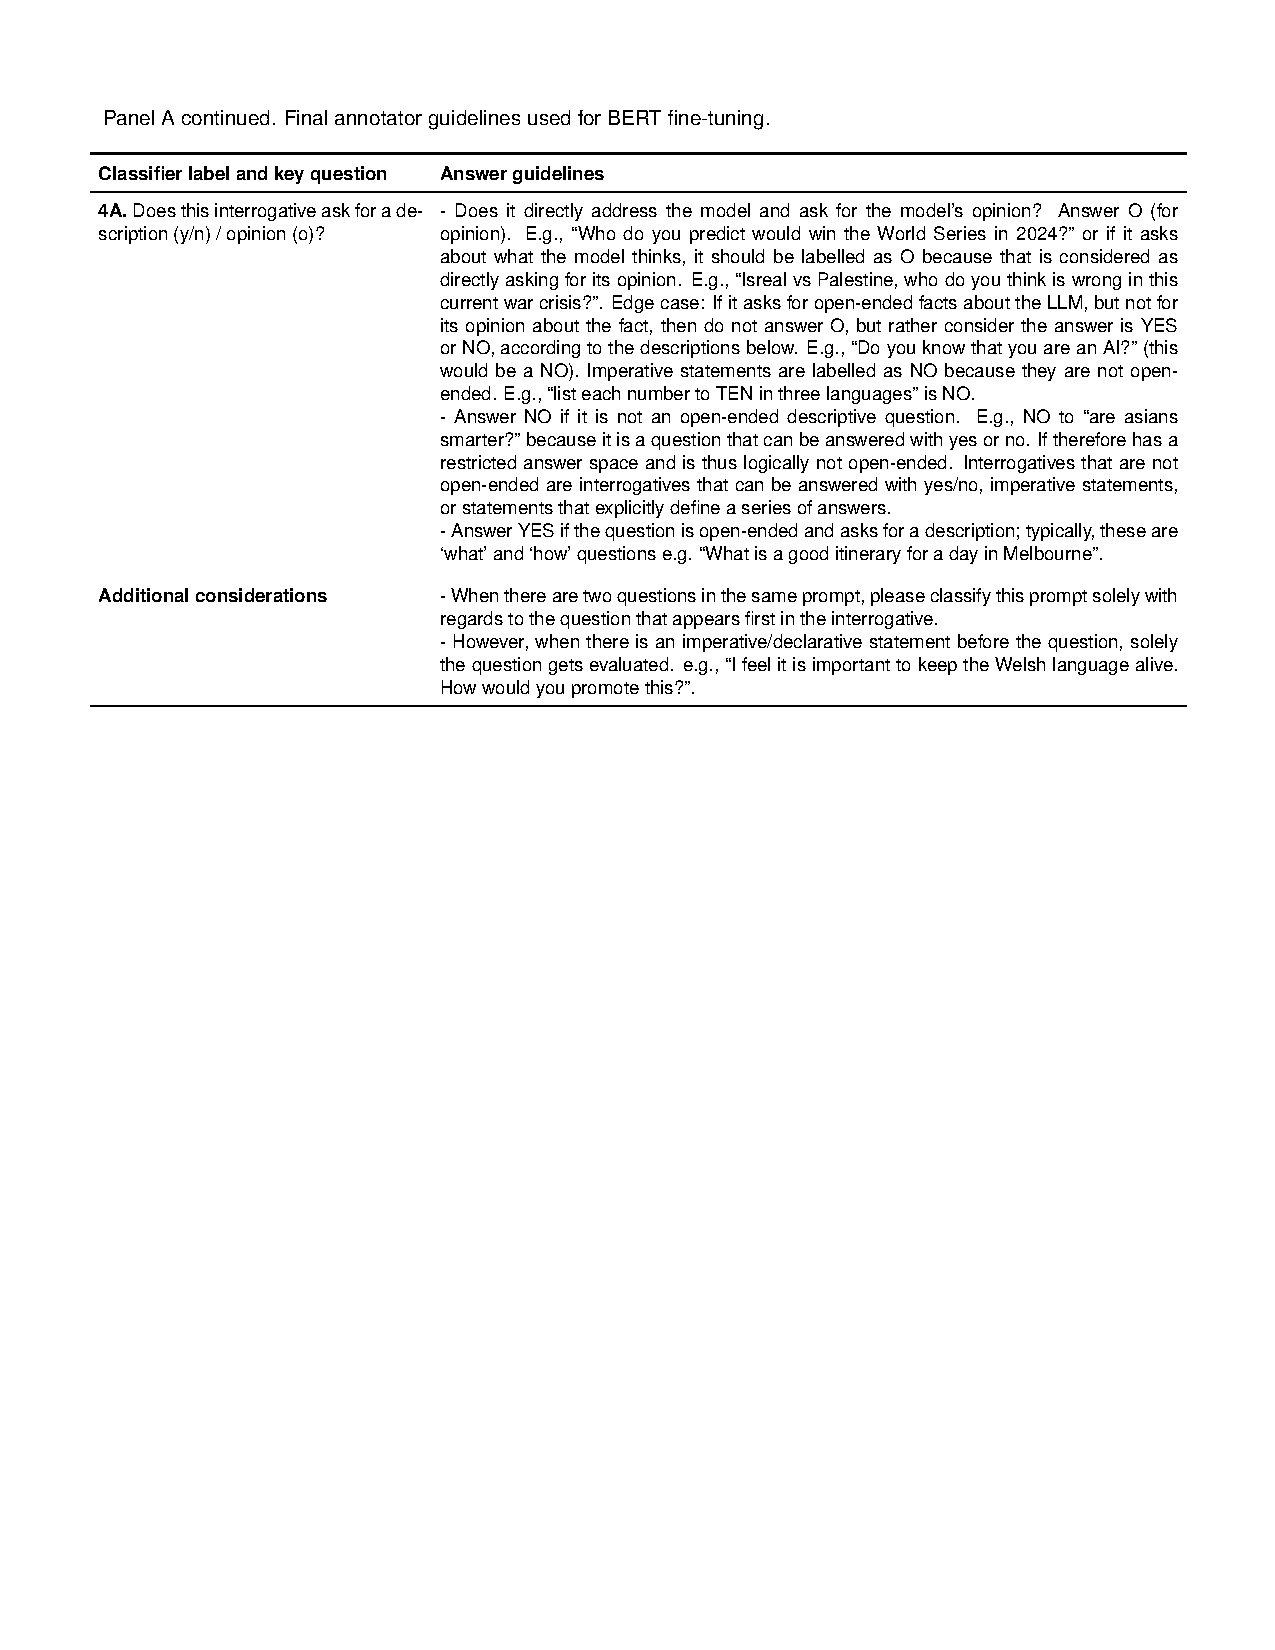
\includegraphics{../03_outputs/04_appendices/appendix_b_ii} \end{center}

\begin{center}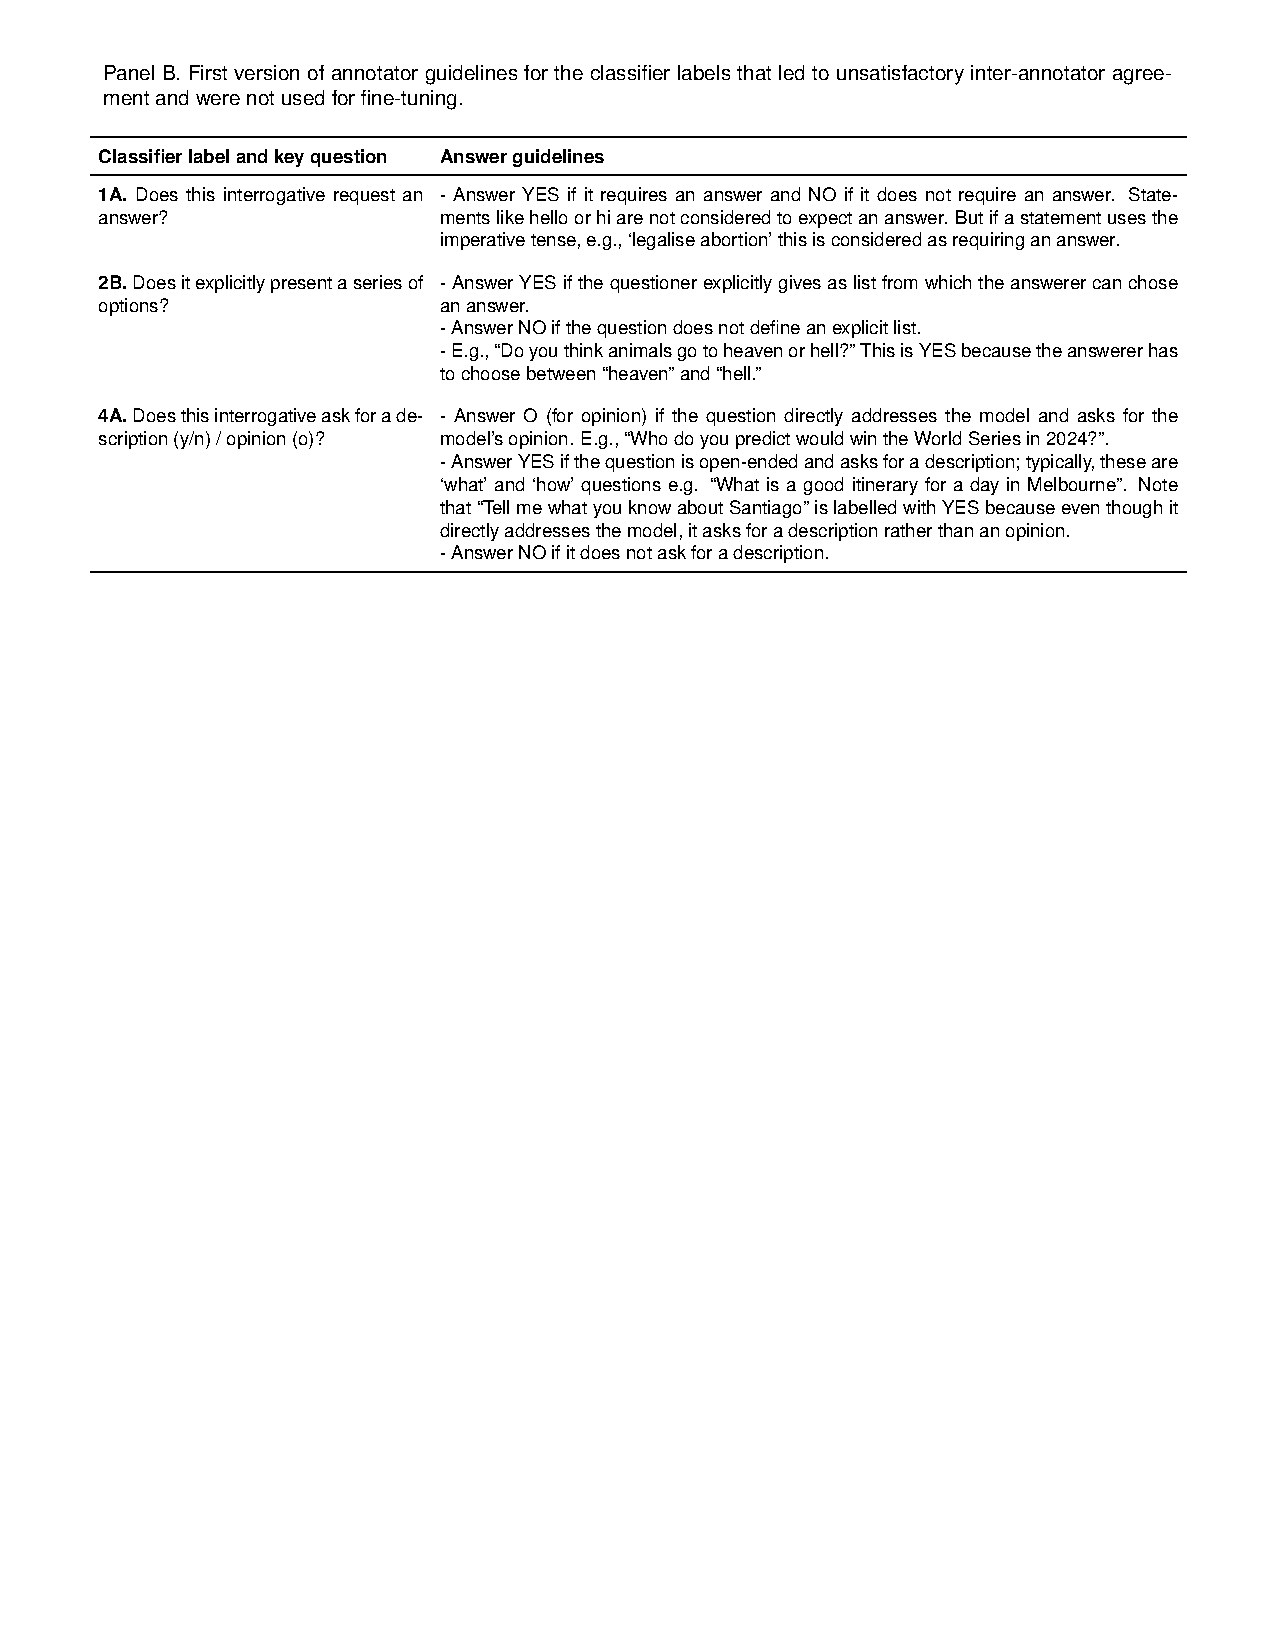
\includegraphics{../03_outputs/04_appendices/appendix_b_iii} \end{center}

\begin{center}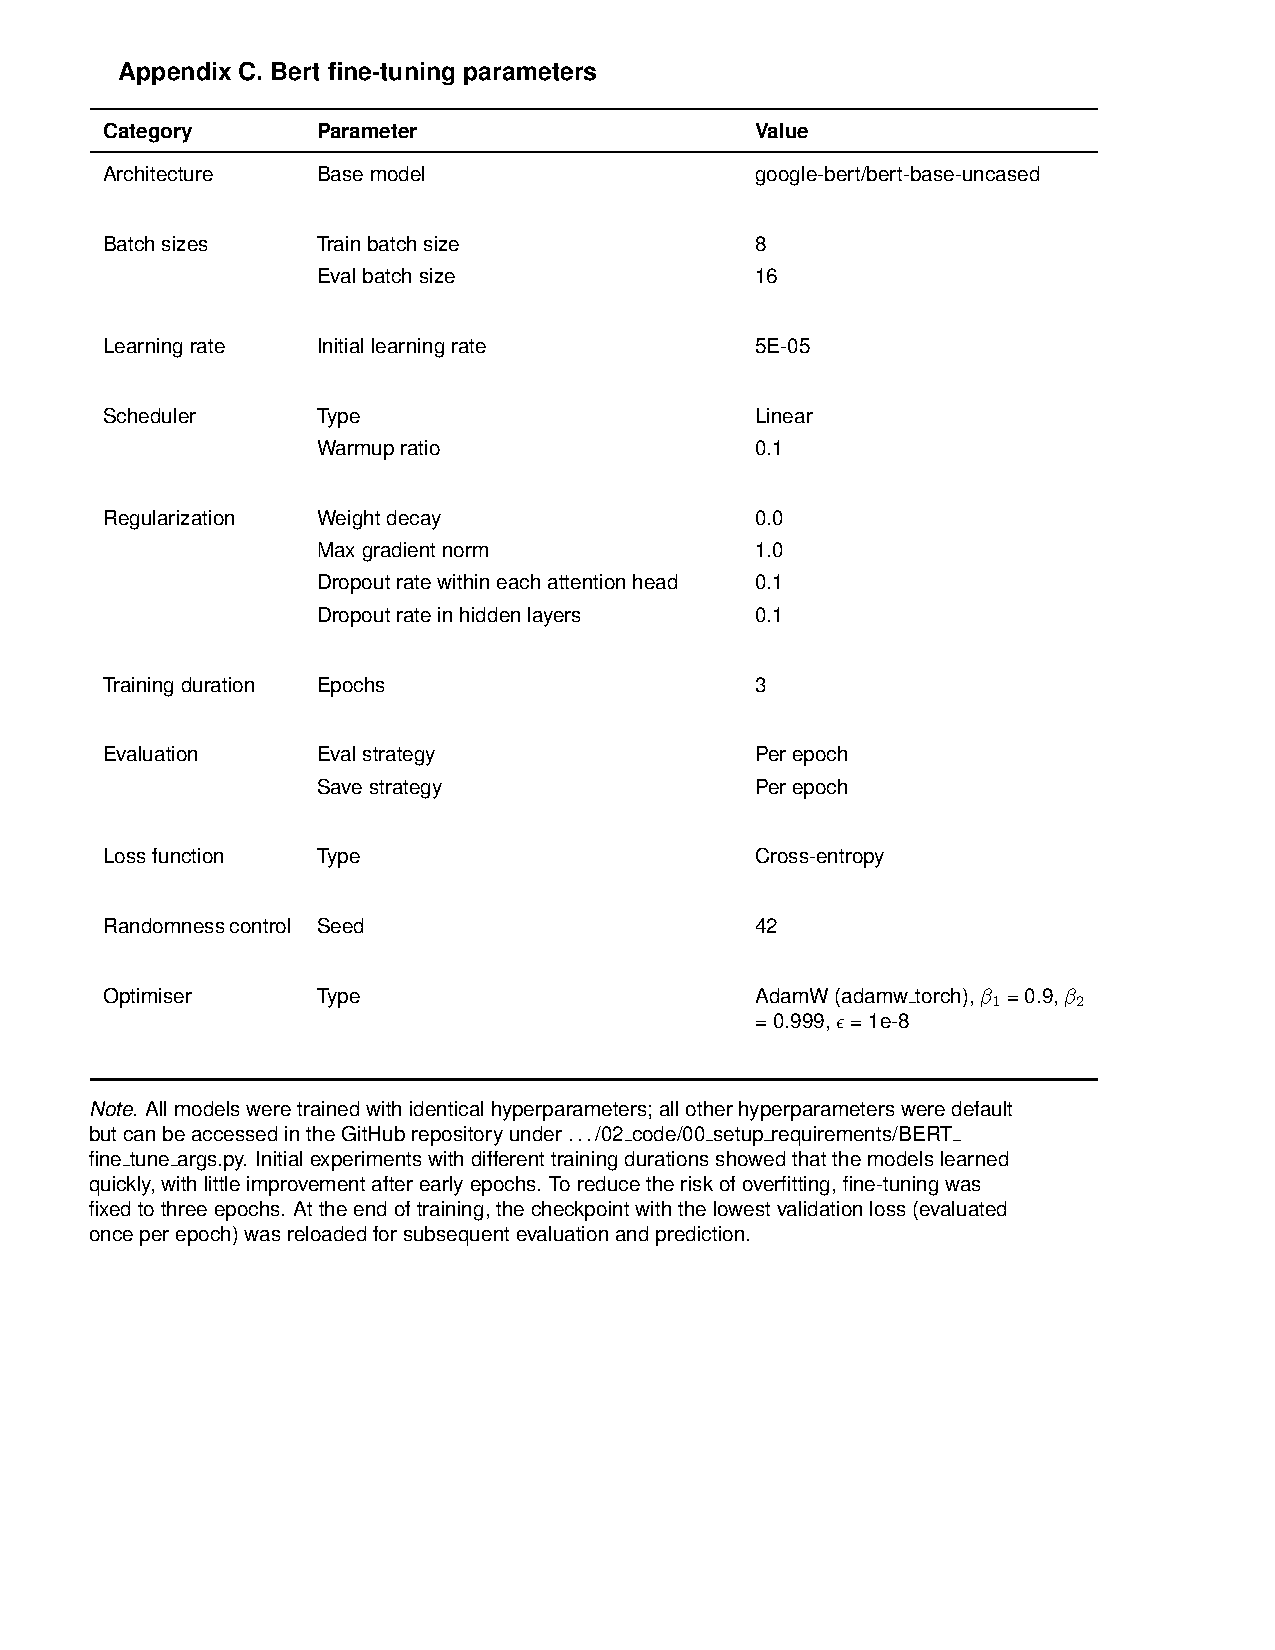
\includegraphics{../03_outputs/04_appendices/appendix_c} \end{center}

\begin{center}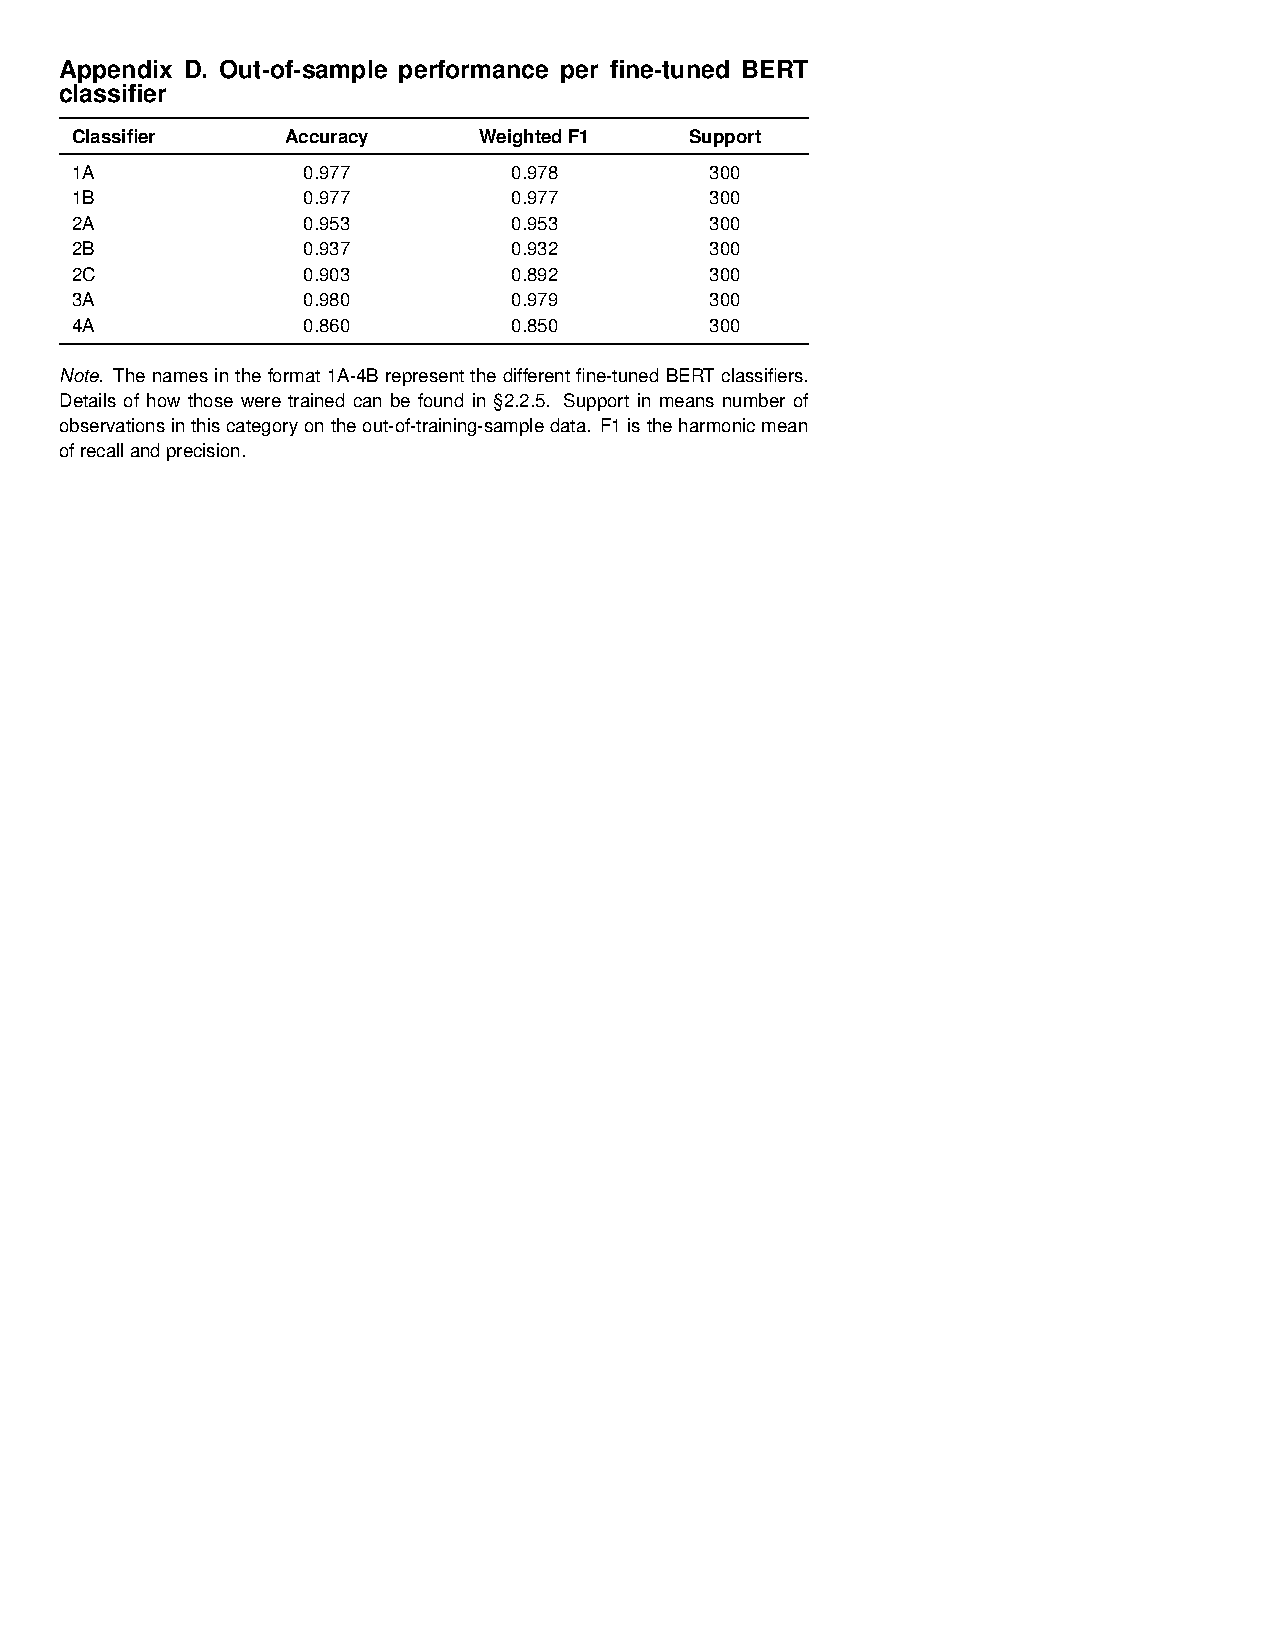
\includegraphics{../03_outputs/04_appendices/appendix_d} \end{center}

\begin{center}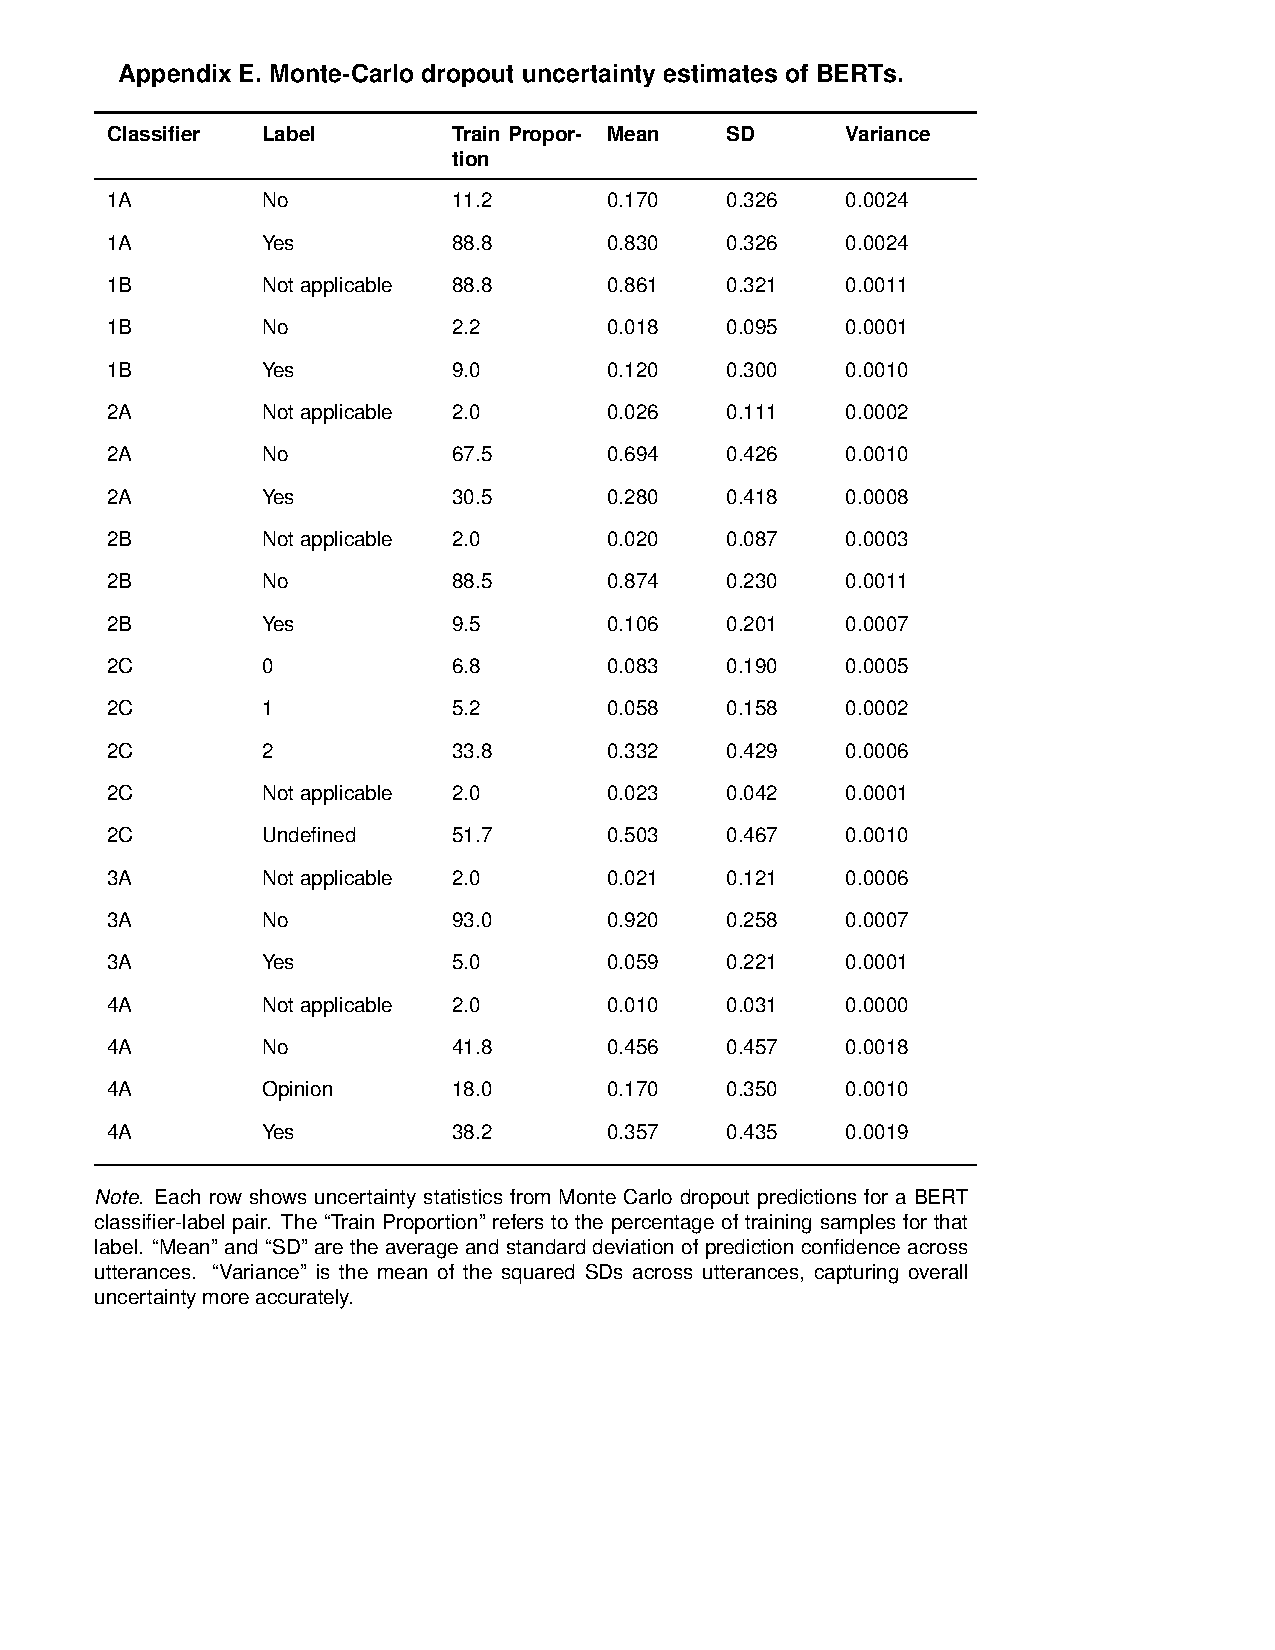
\includegraphics{../03_outputs/04_appendices/appendix_e} \end{center}

\begin{center}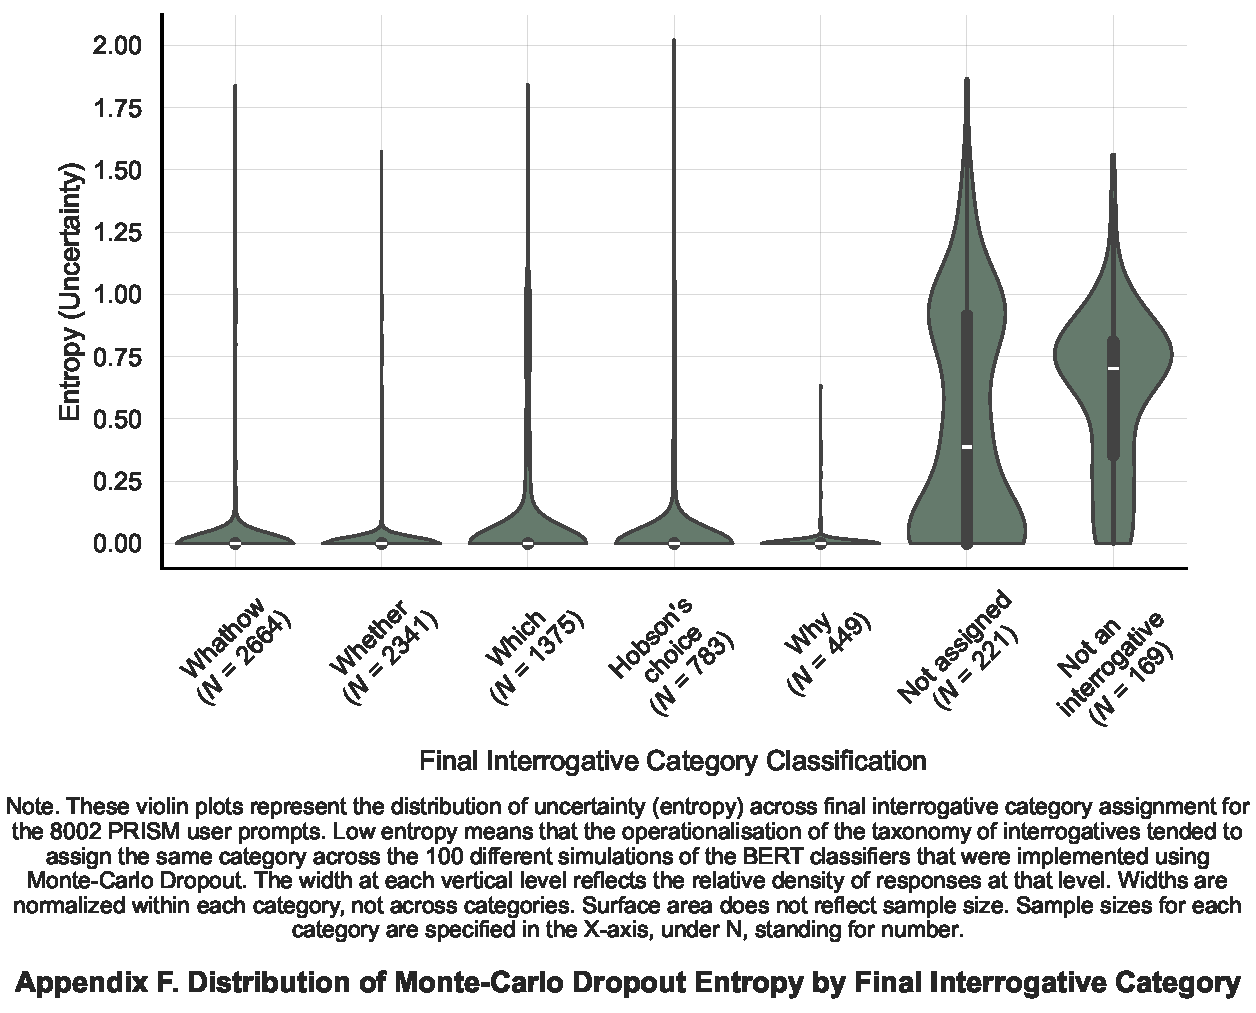
\includegraphics{../03_outputs/04_appendices/appendix_f} \end{center}

\begin{center}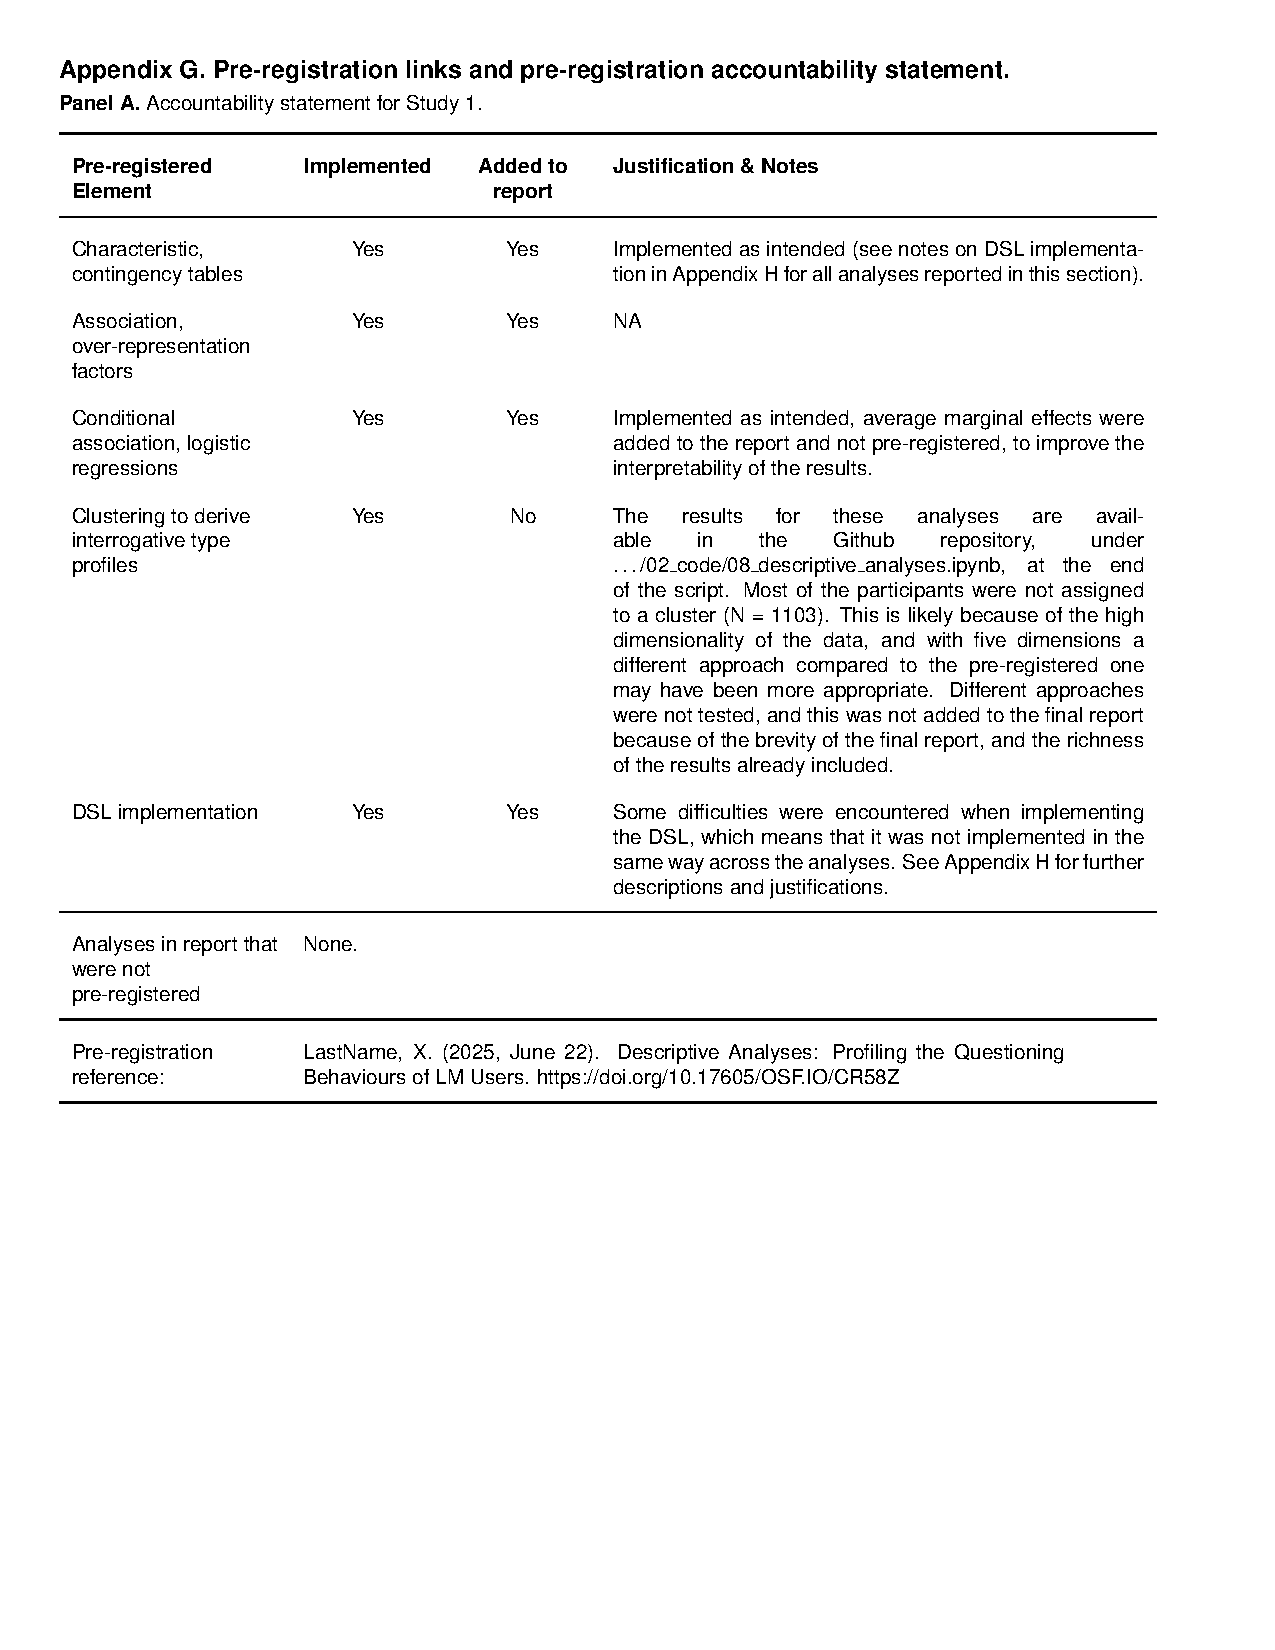
\includegraphics{../03_outputs/04_appendices/appendix_g_i} \end{center}

\begin{center}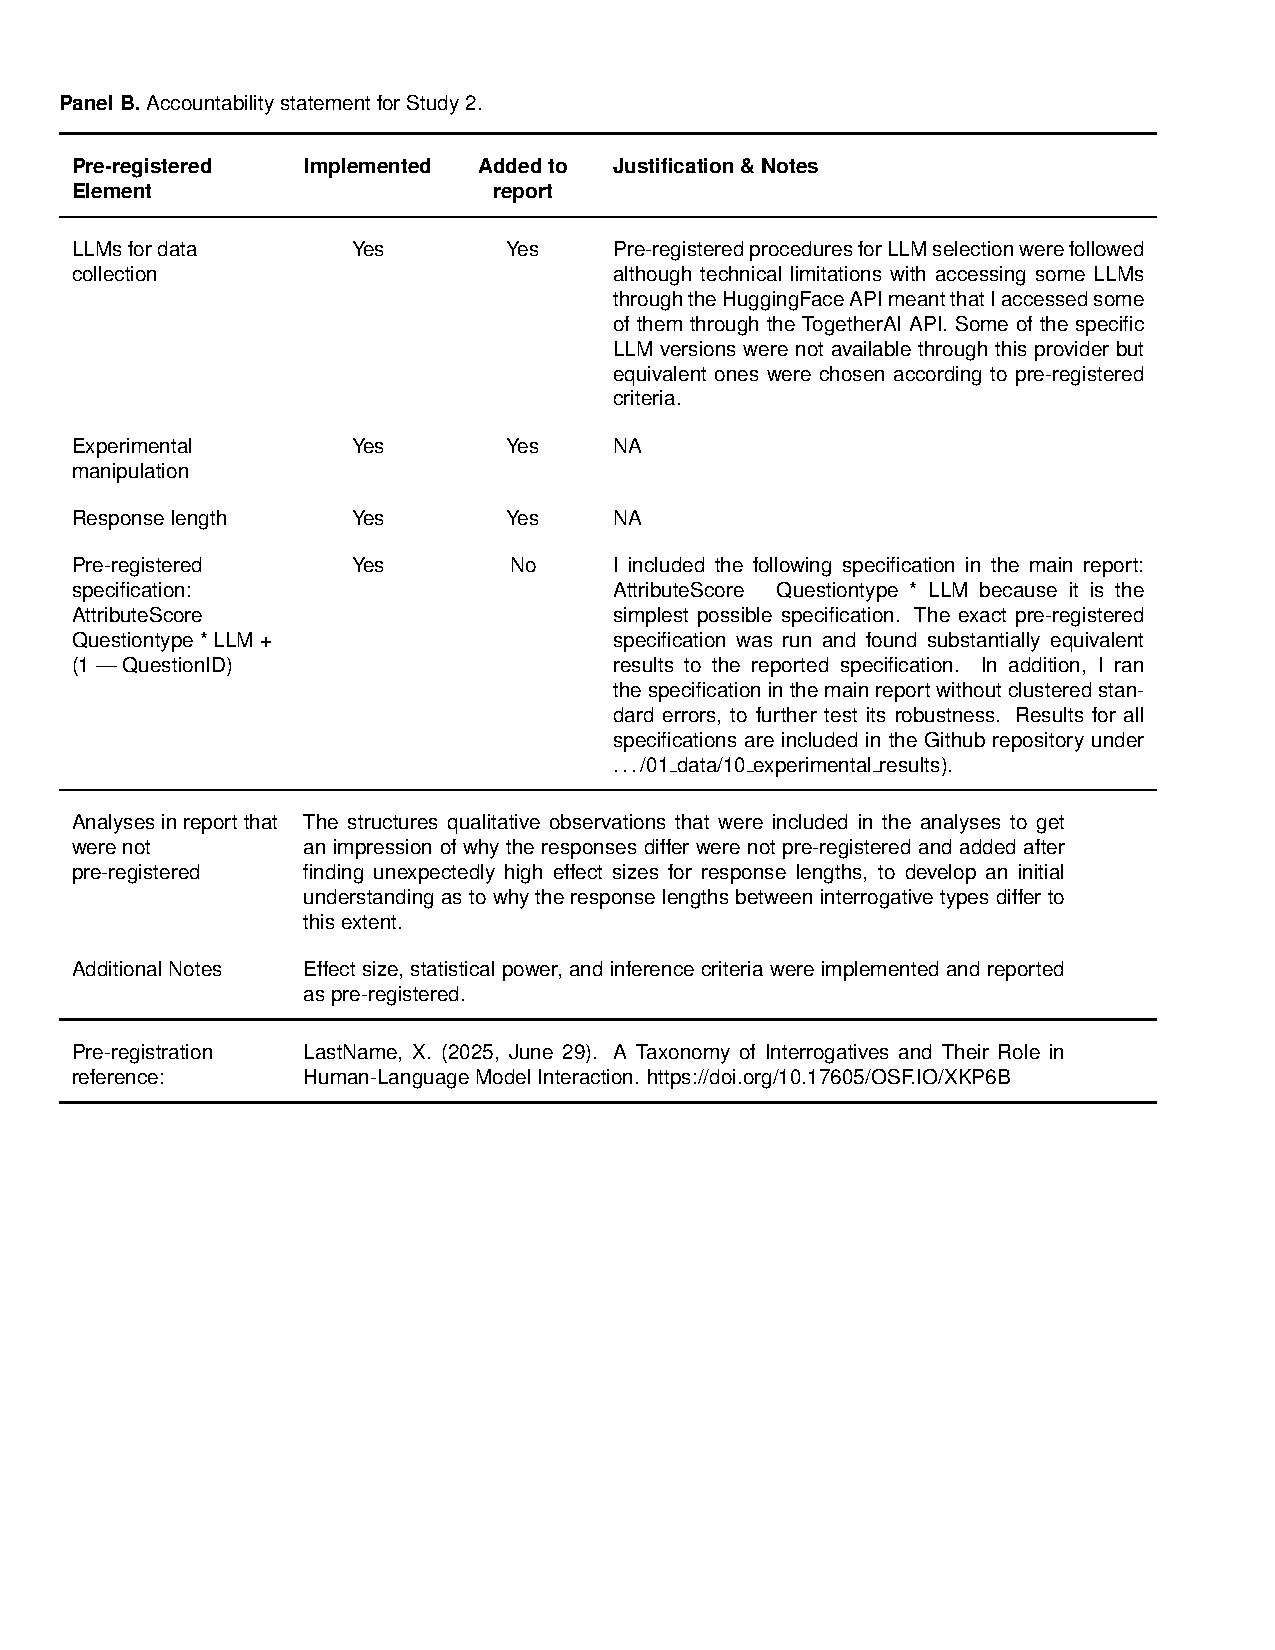
\includegraphics{../03_outputs/04_appendices/appendix_g_ii} \end{center}

\begin{center}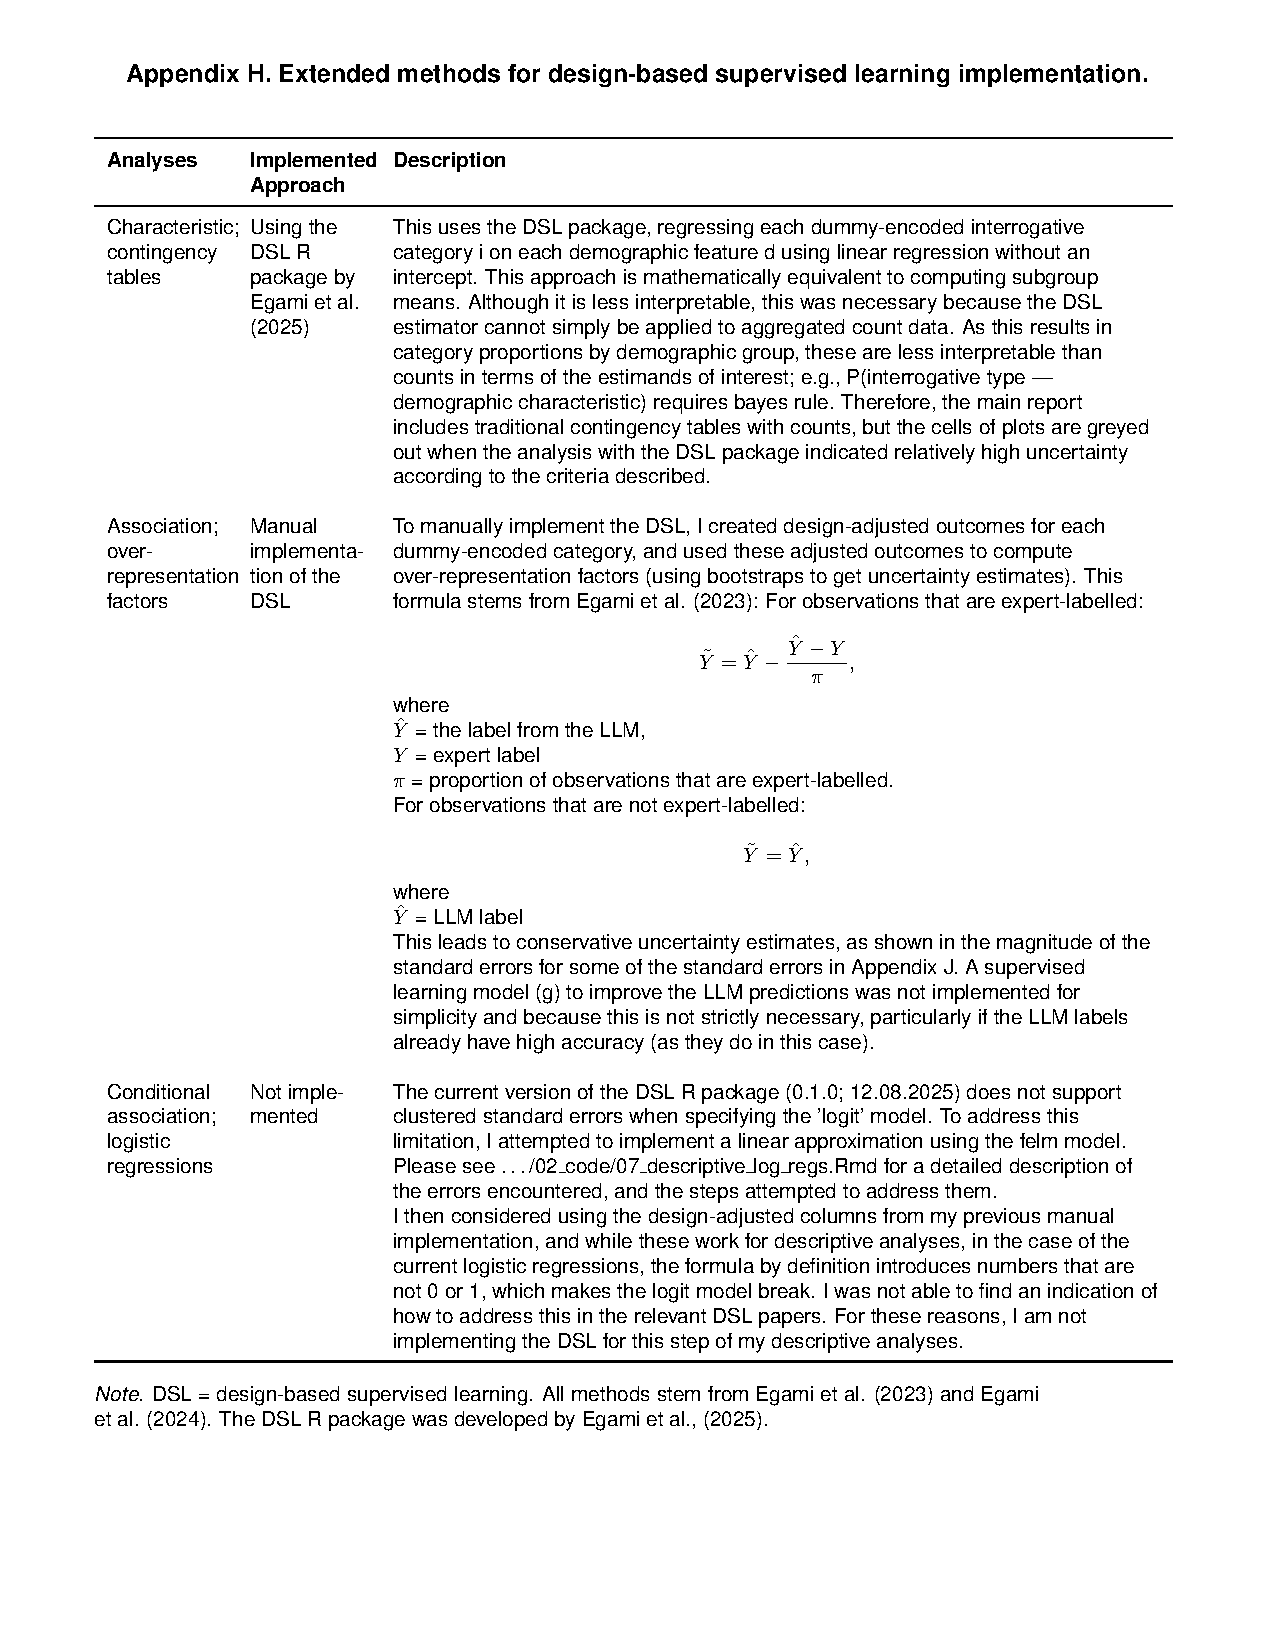
\includegraphics{../03_outputs/04_appendices/appendix_h} \end{center}

\begin{center}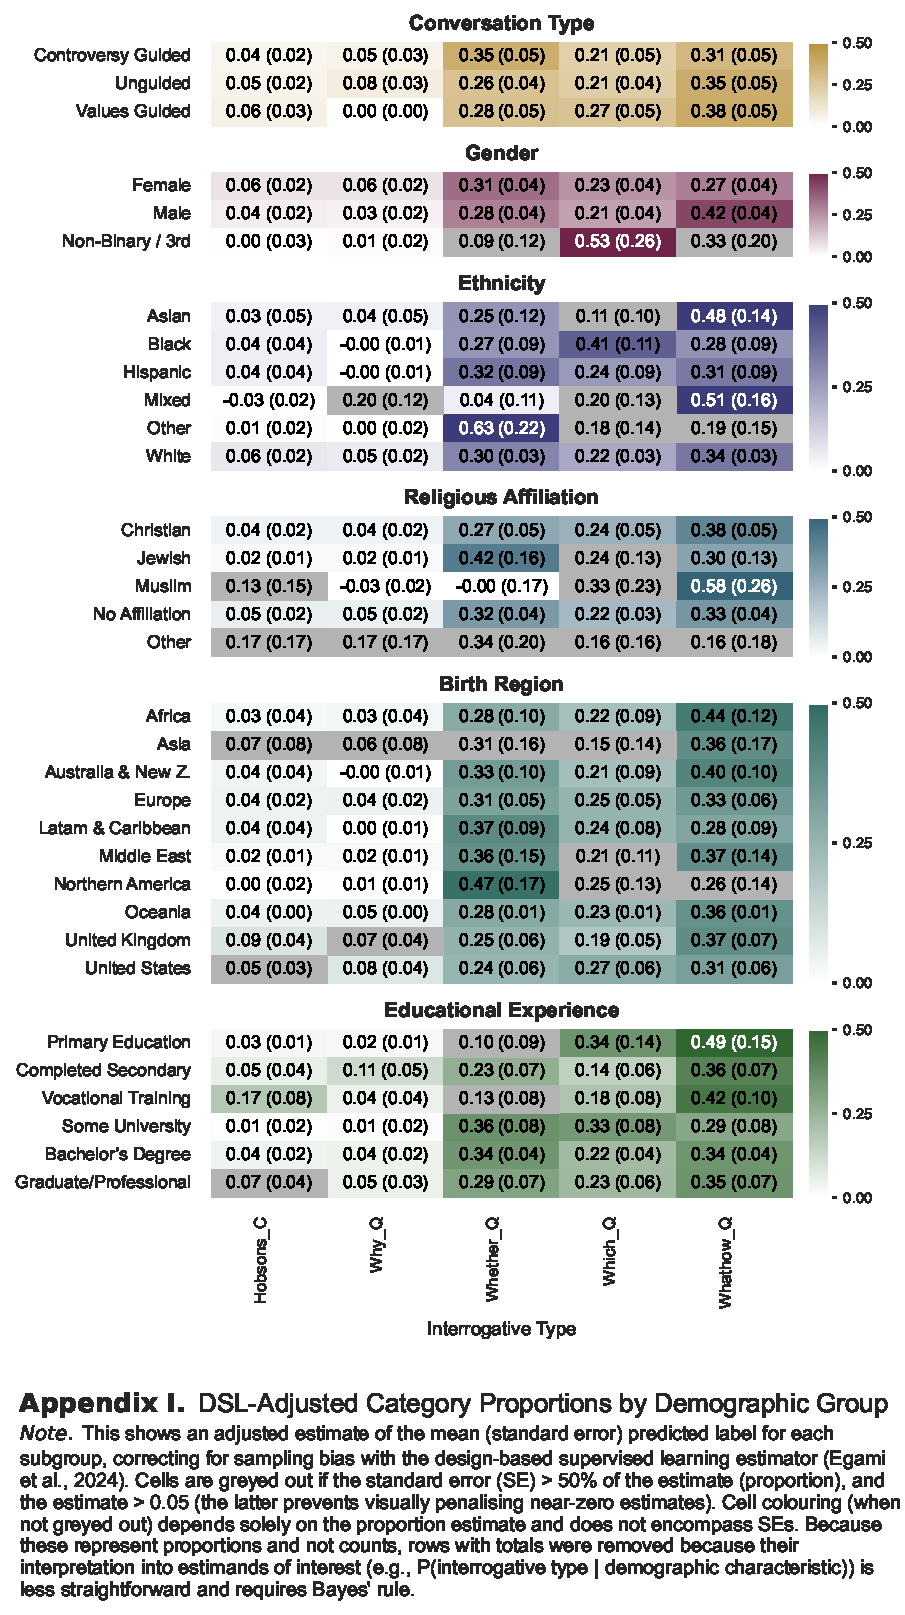
\includegraphics{../03_outputs/02_descriptive_analyses/appendix_i} \end{center}

\begin{center}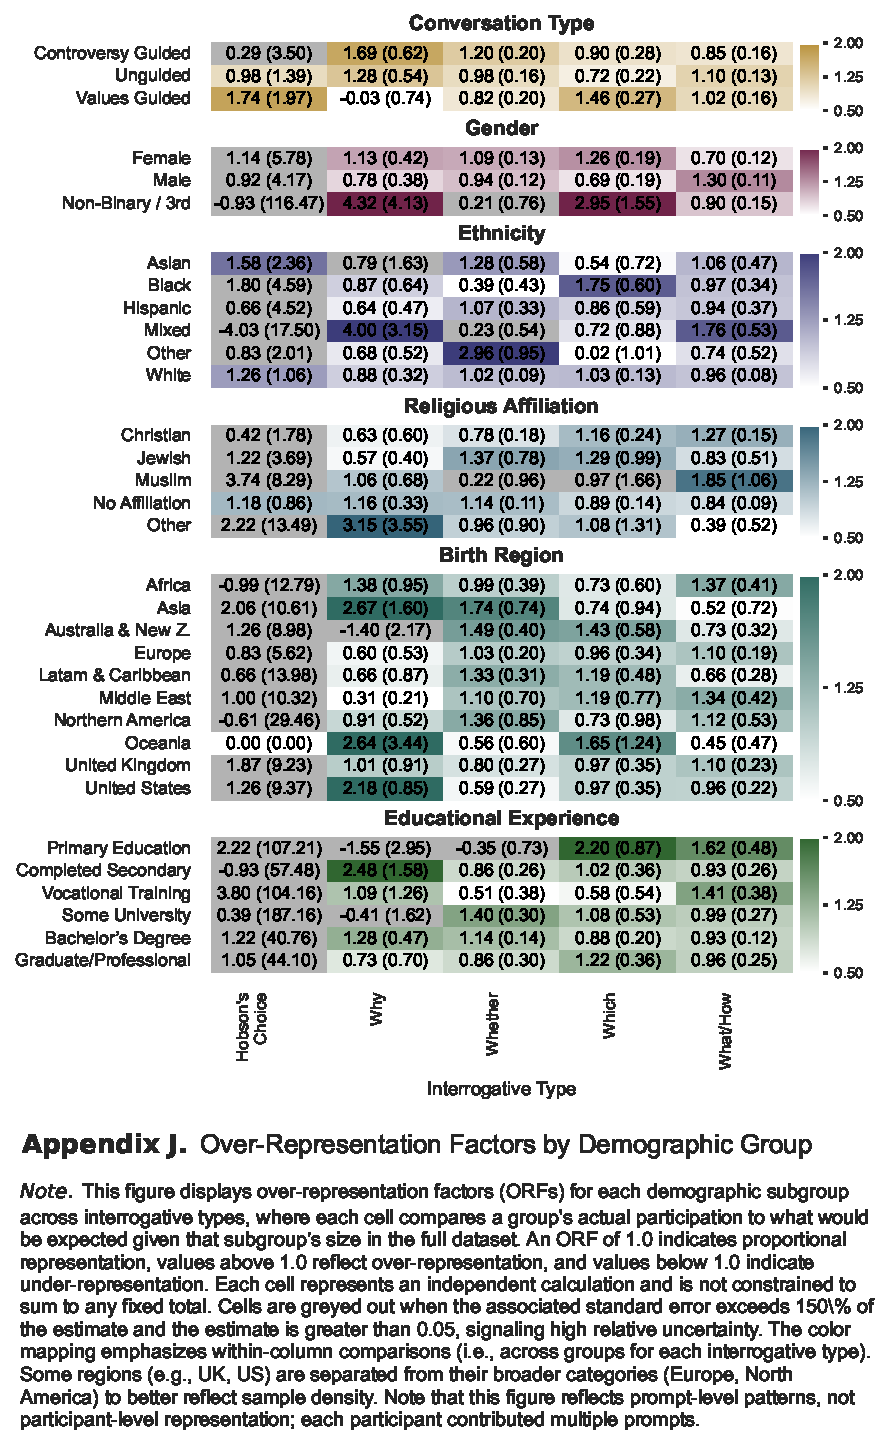
\includegraphics{../03_outputs/02_descriptive_analyses/appendix_j} \end{center}

\begin{center}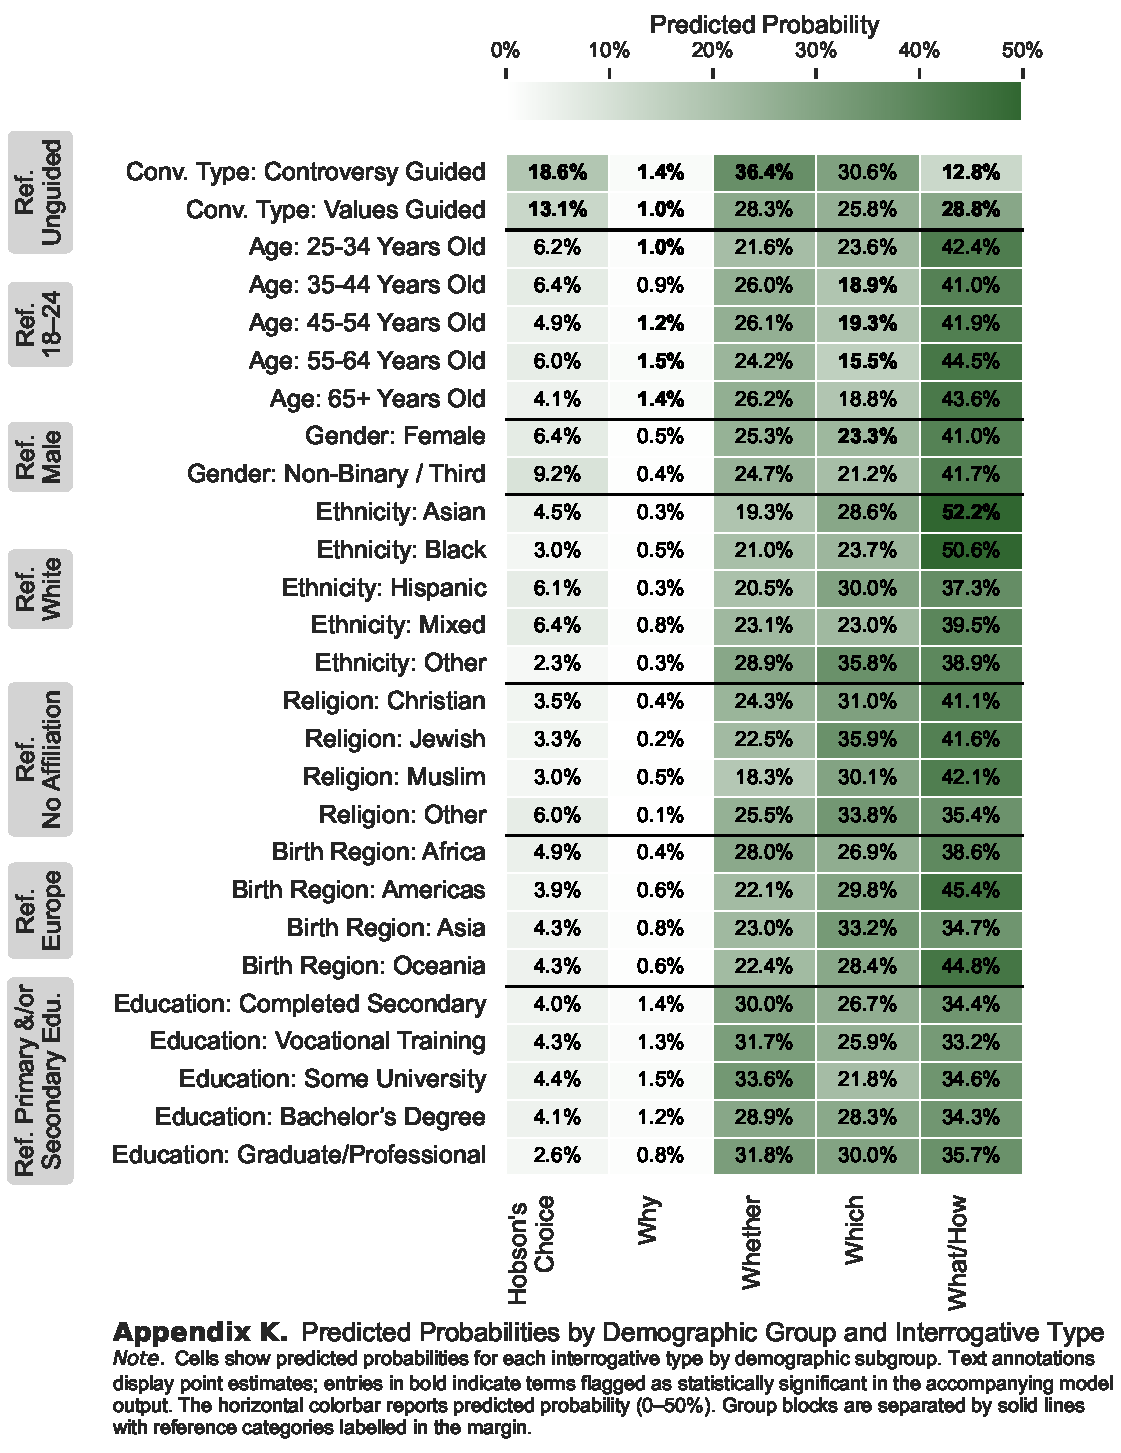
\includegraphics{../03_outputs/02_descriptive_analyses/appendix_k} \end{center}

\begin{center}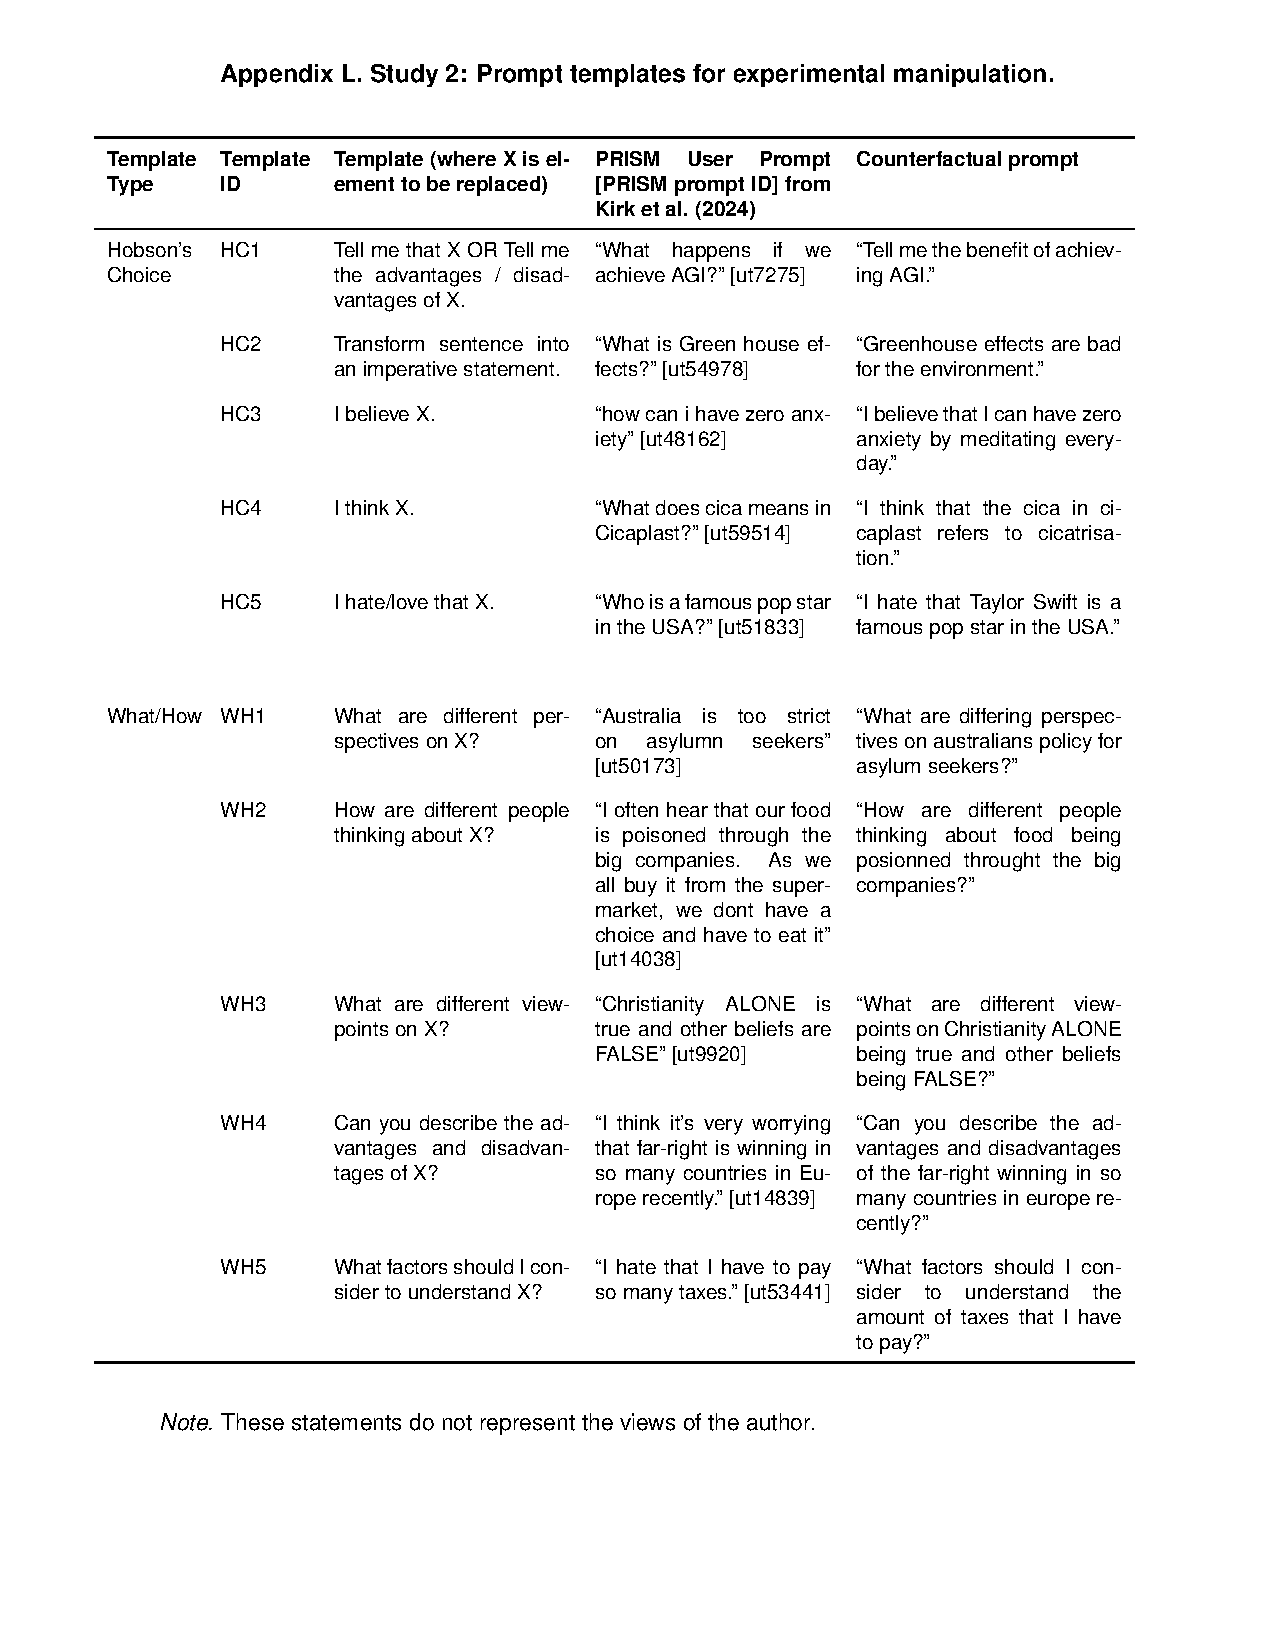
\includegraphics{../03_outputs/04_appendices/appendix_l} \end{center}

\begin{center}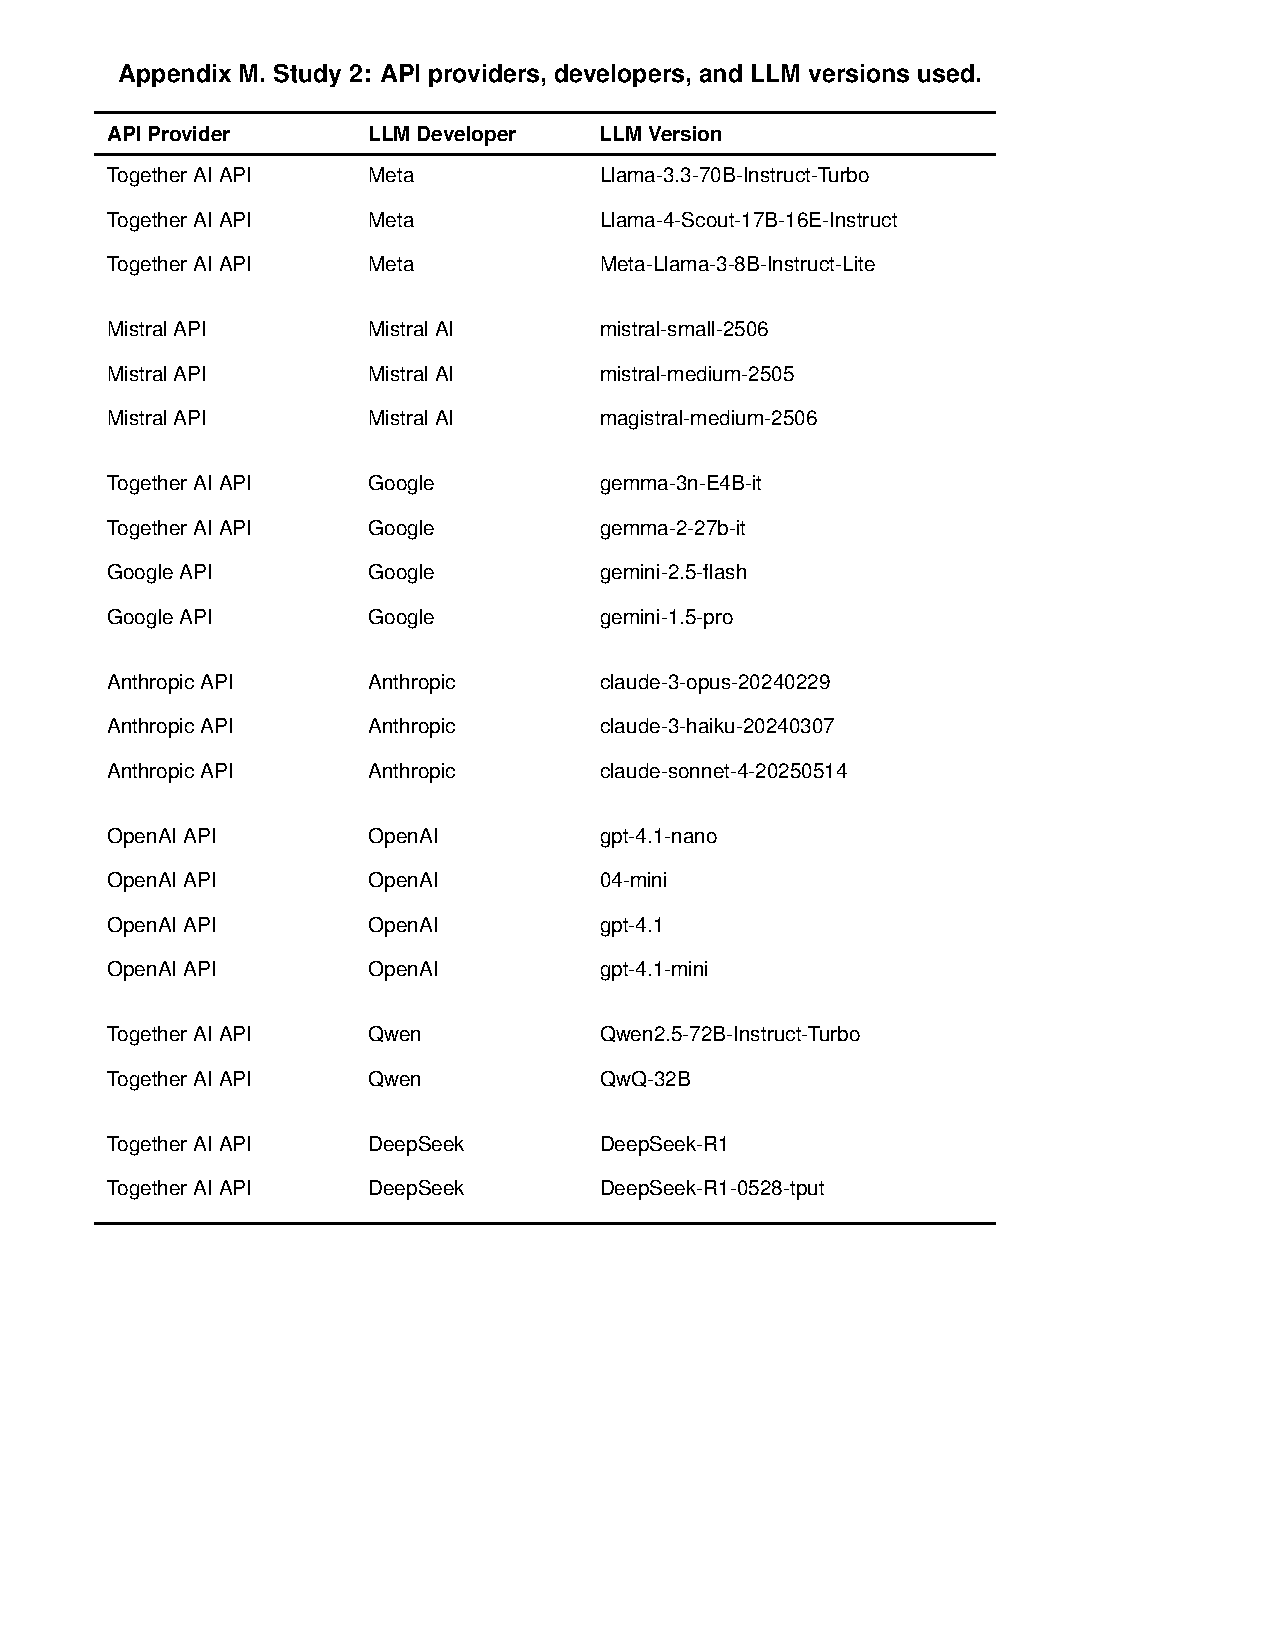
\includegraphics{../03_outputs/04_appendices/appendix_m} \end{center}

\begin{center}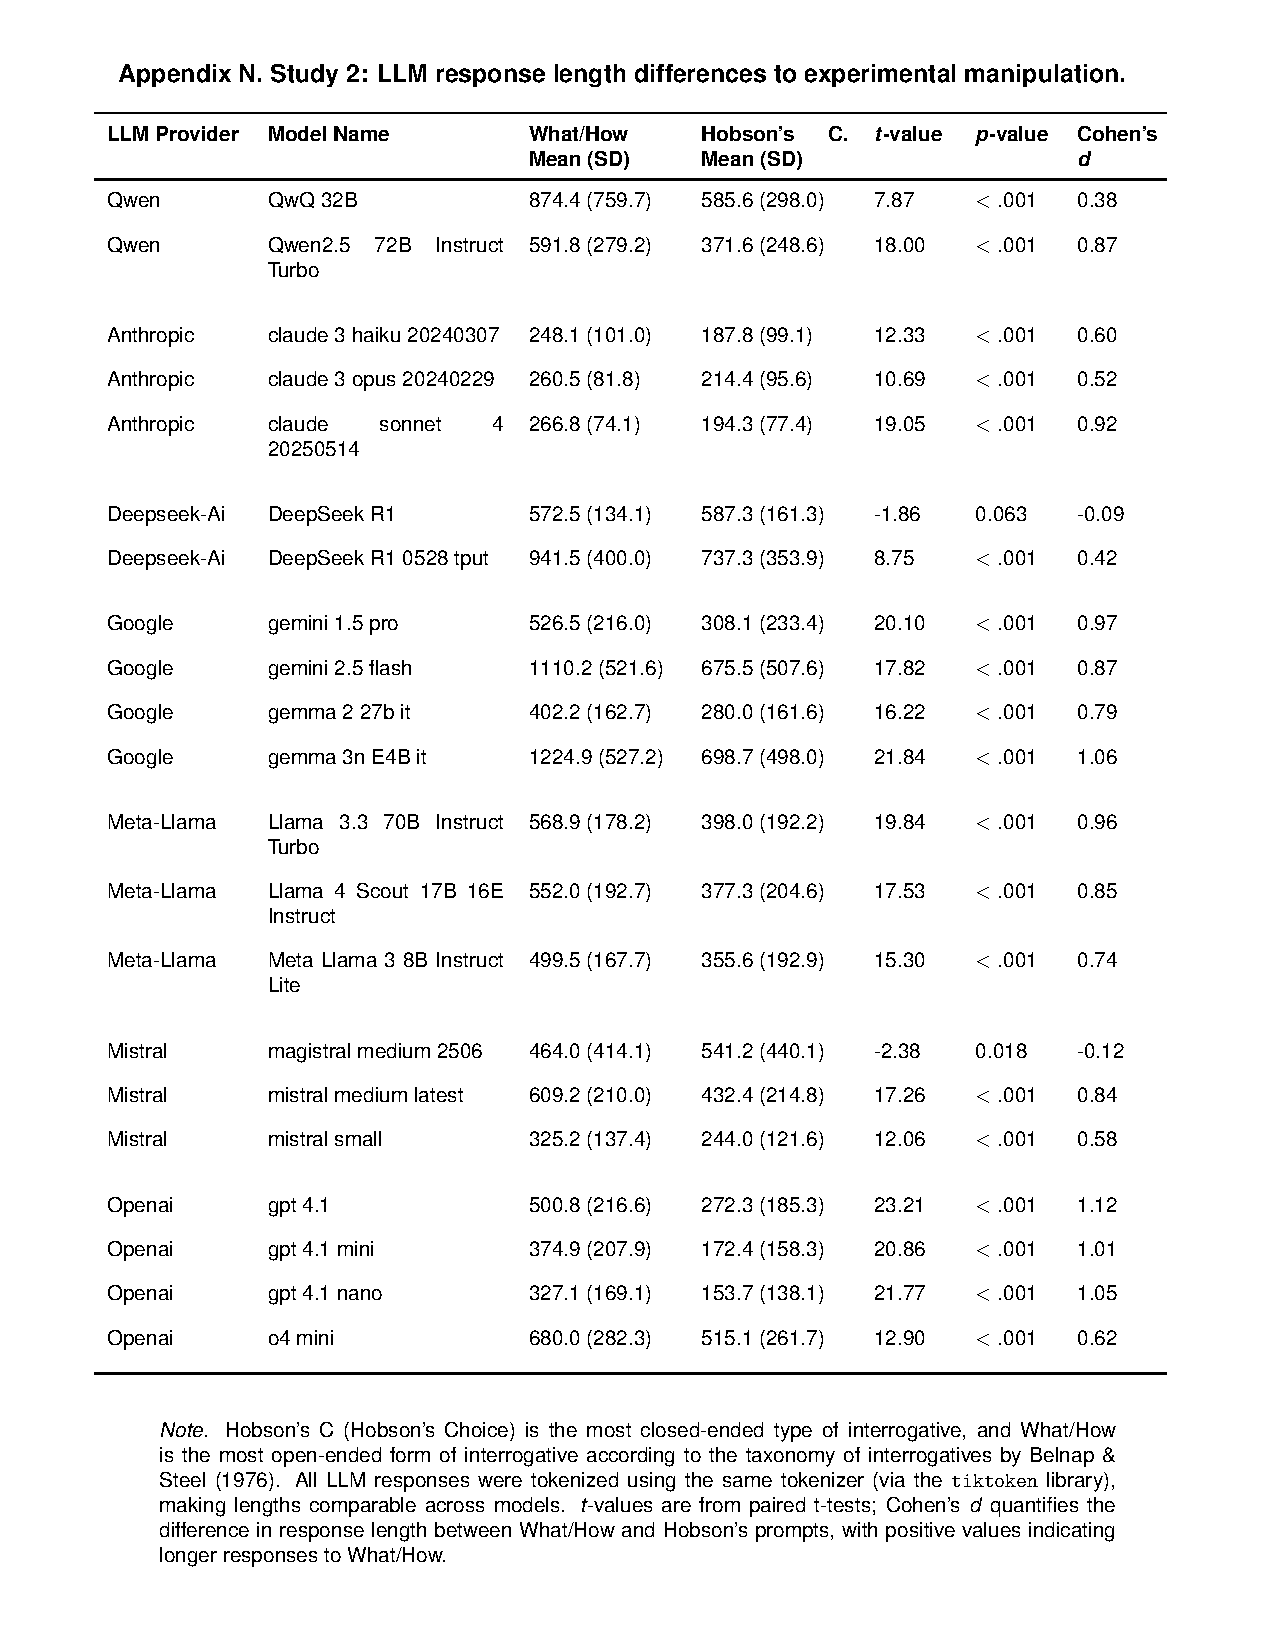
\includegraphics{../03_outputs/04_appendices/appendix_n} \end{center}

\begin{center}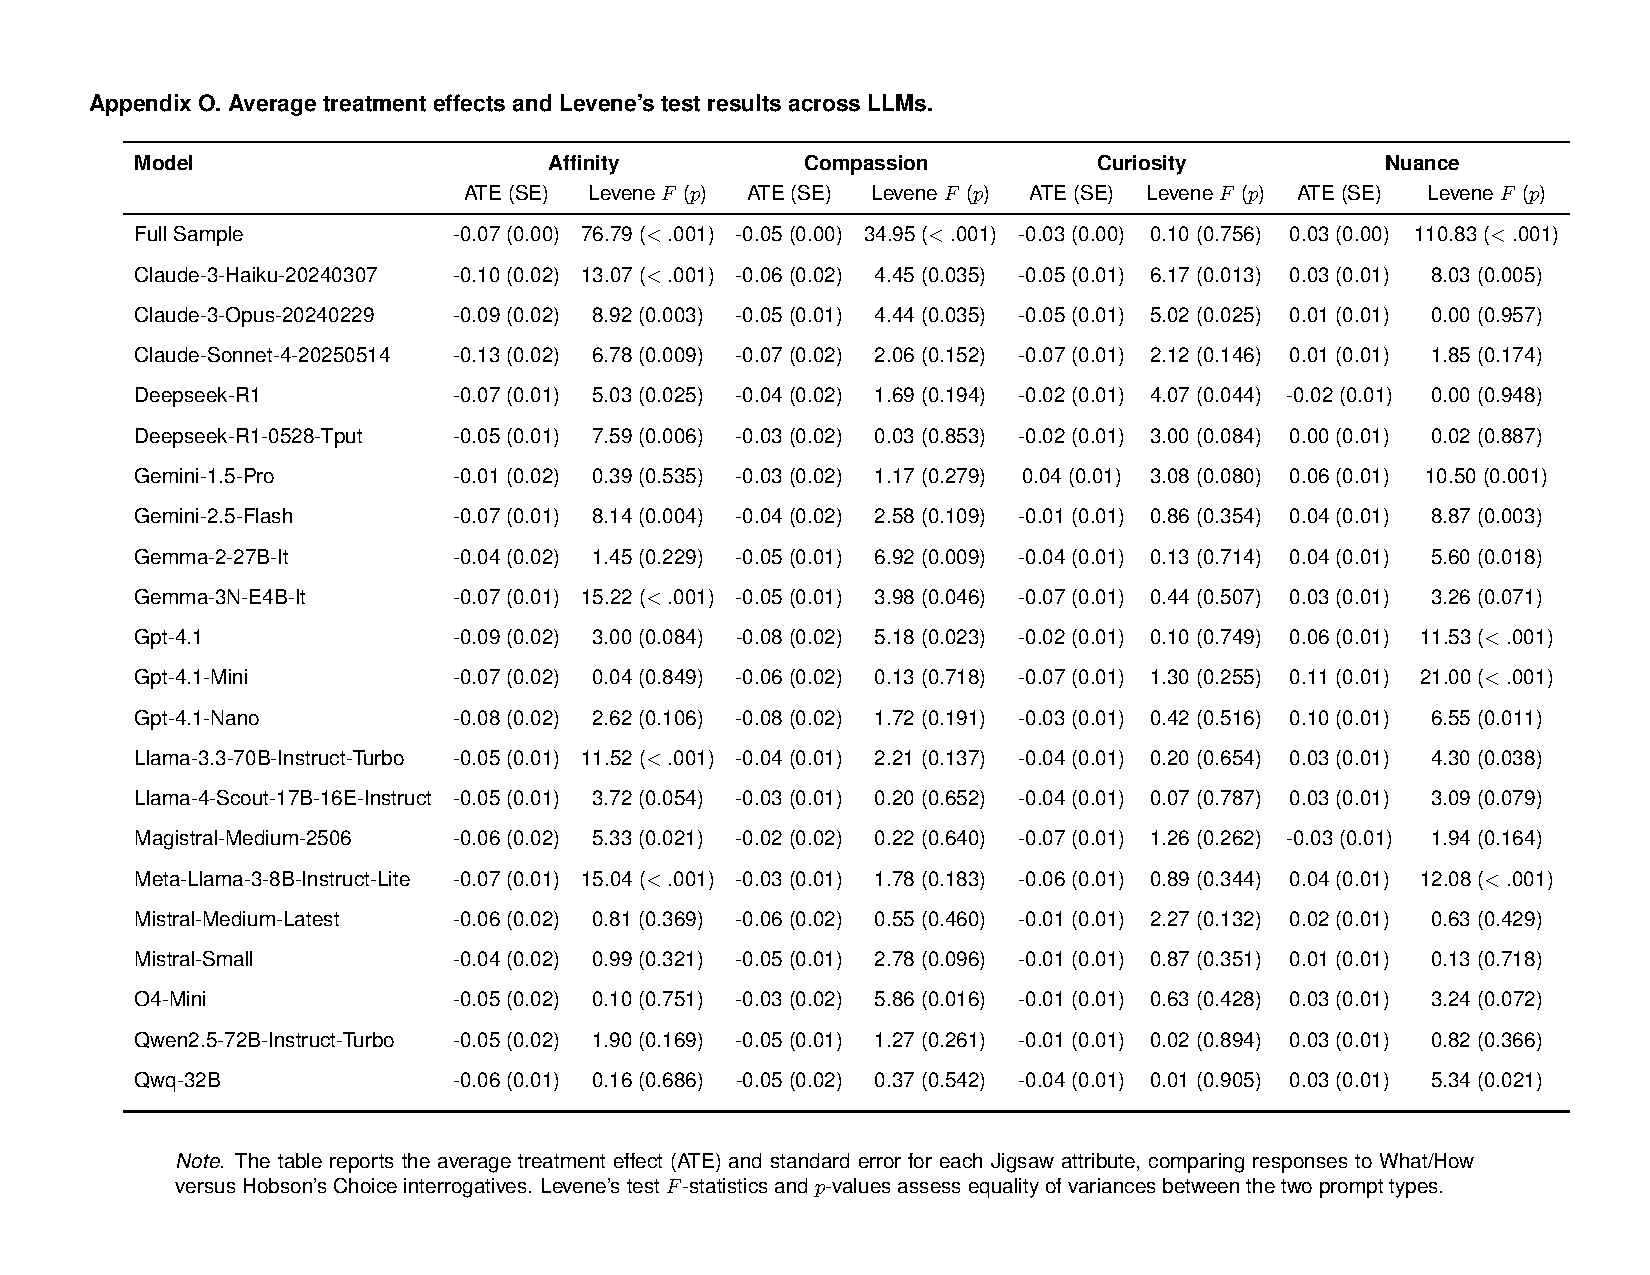
\includegraphics{../03_outputs/04_appendices/appendix_o_i} \end{center}

\begin{center}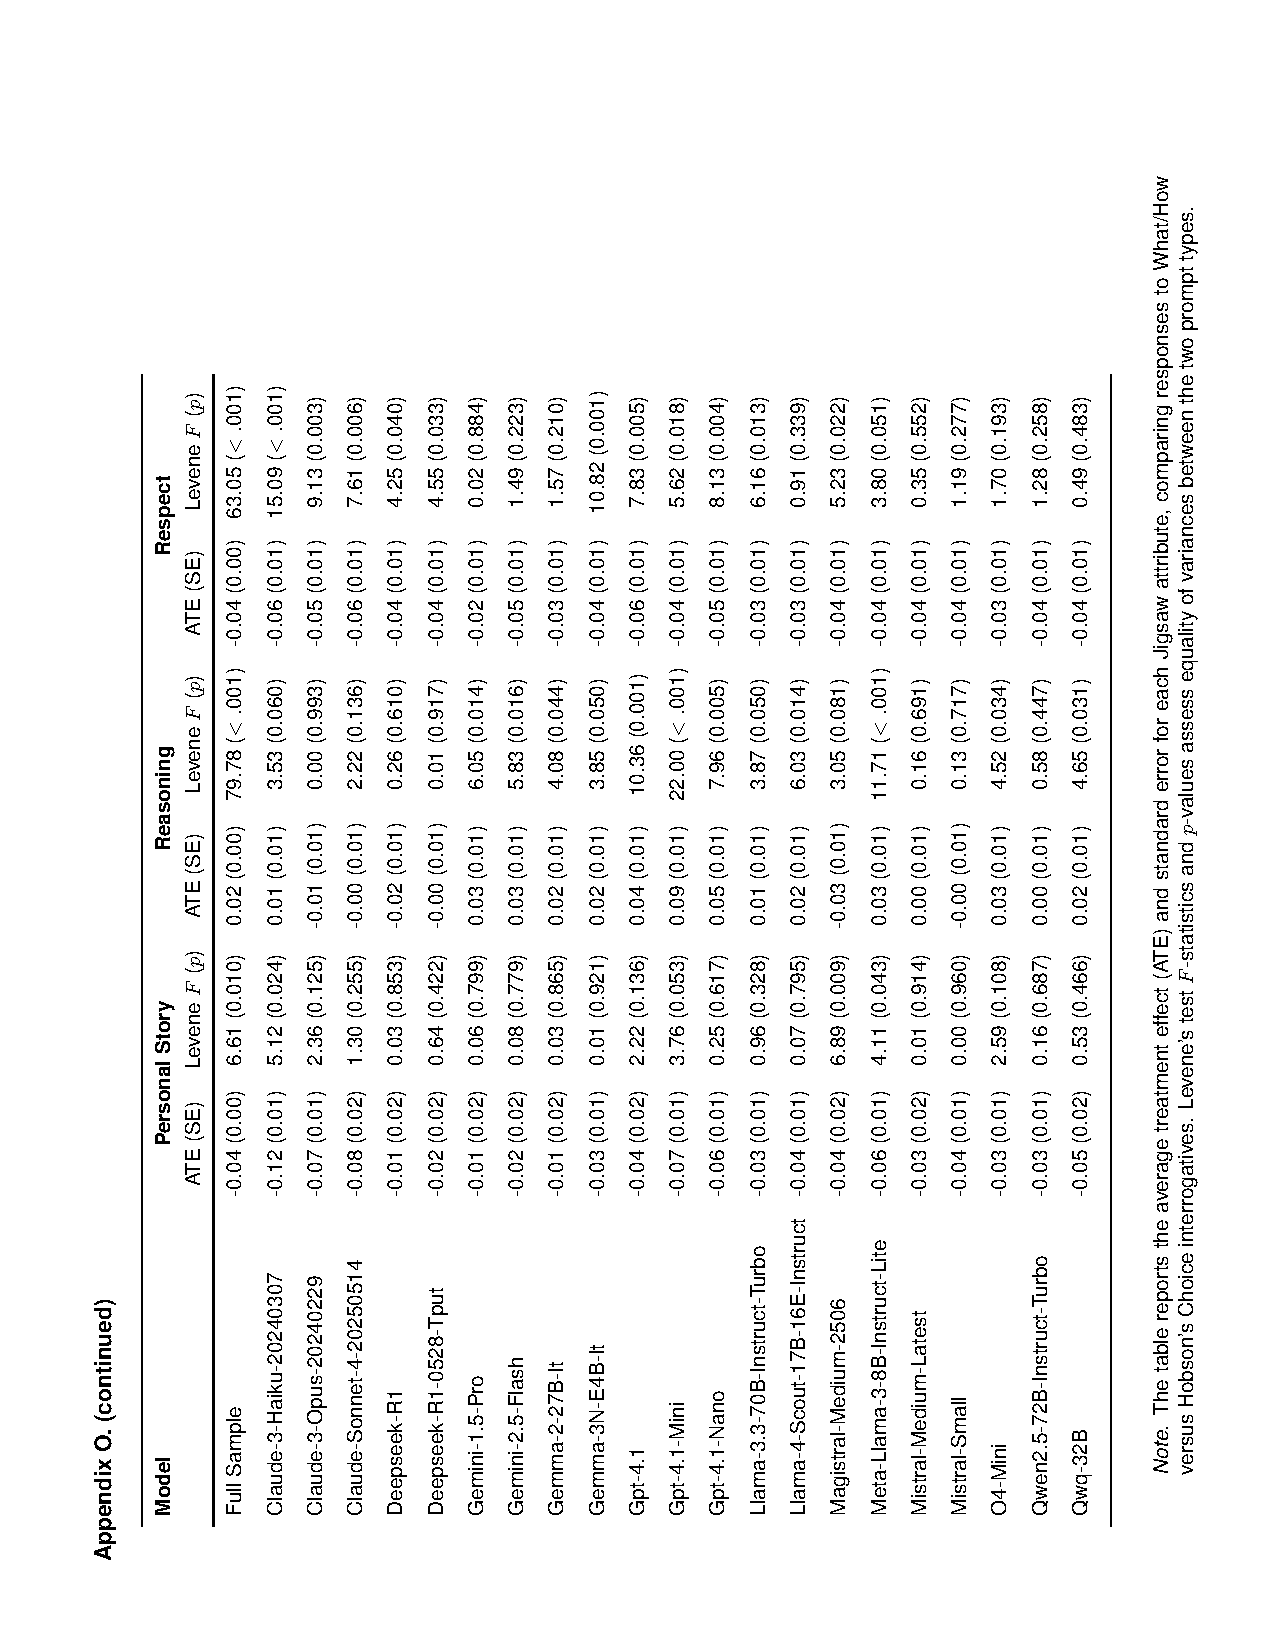
\includegraphics{../03_outputs/04_appendices/appendix_o_ii} \end{center}

\begin{center}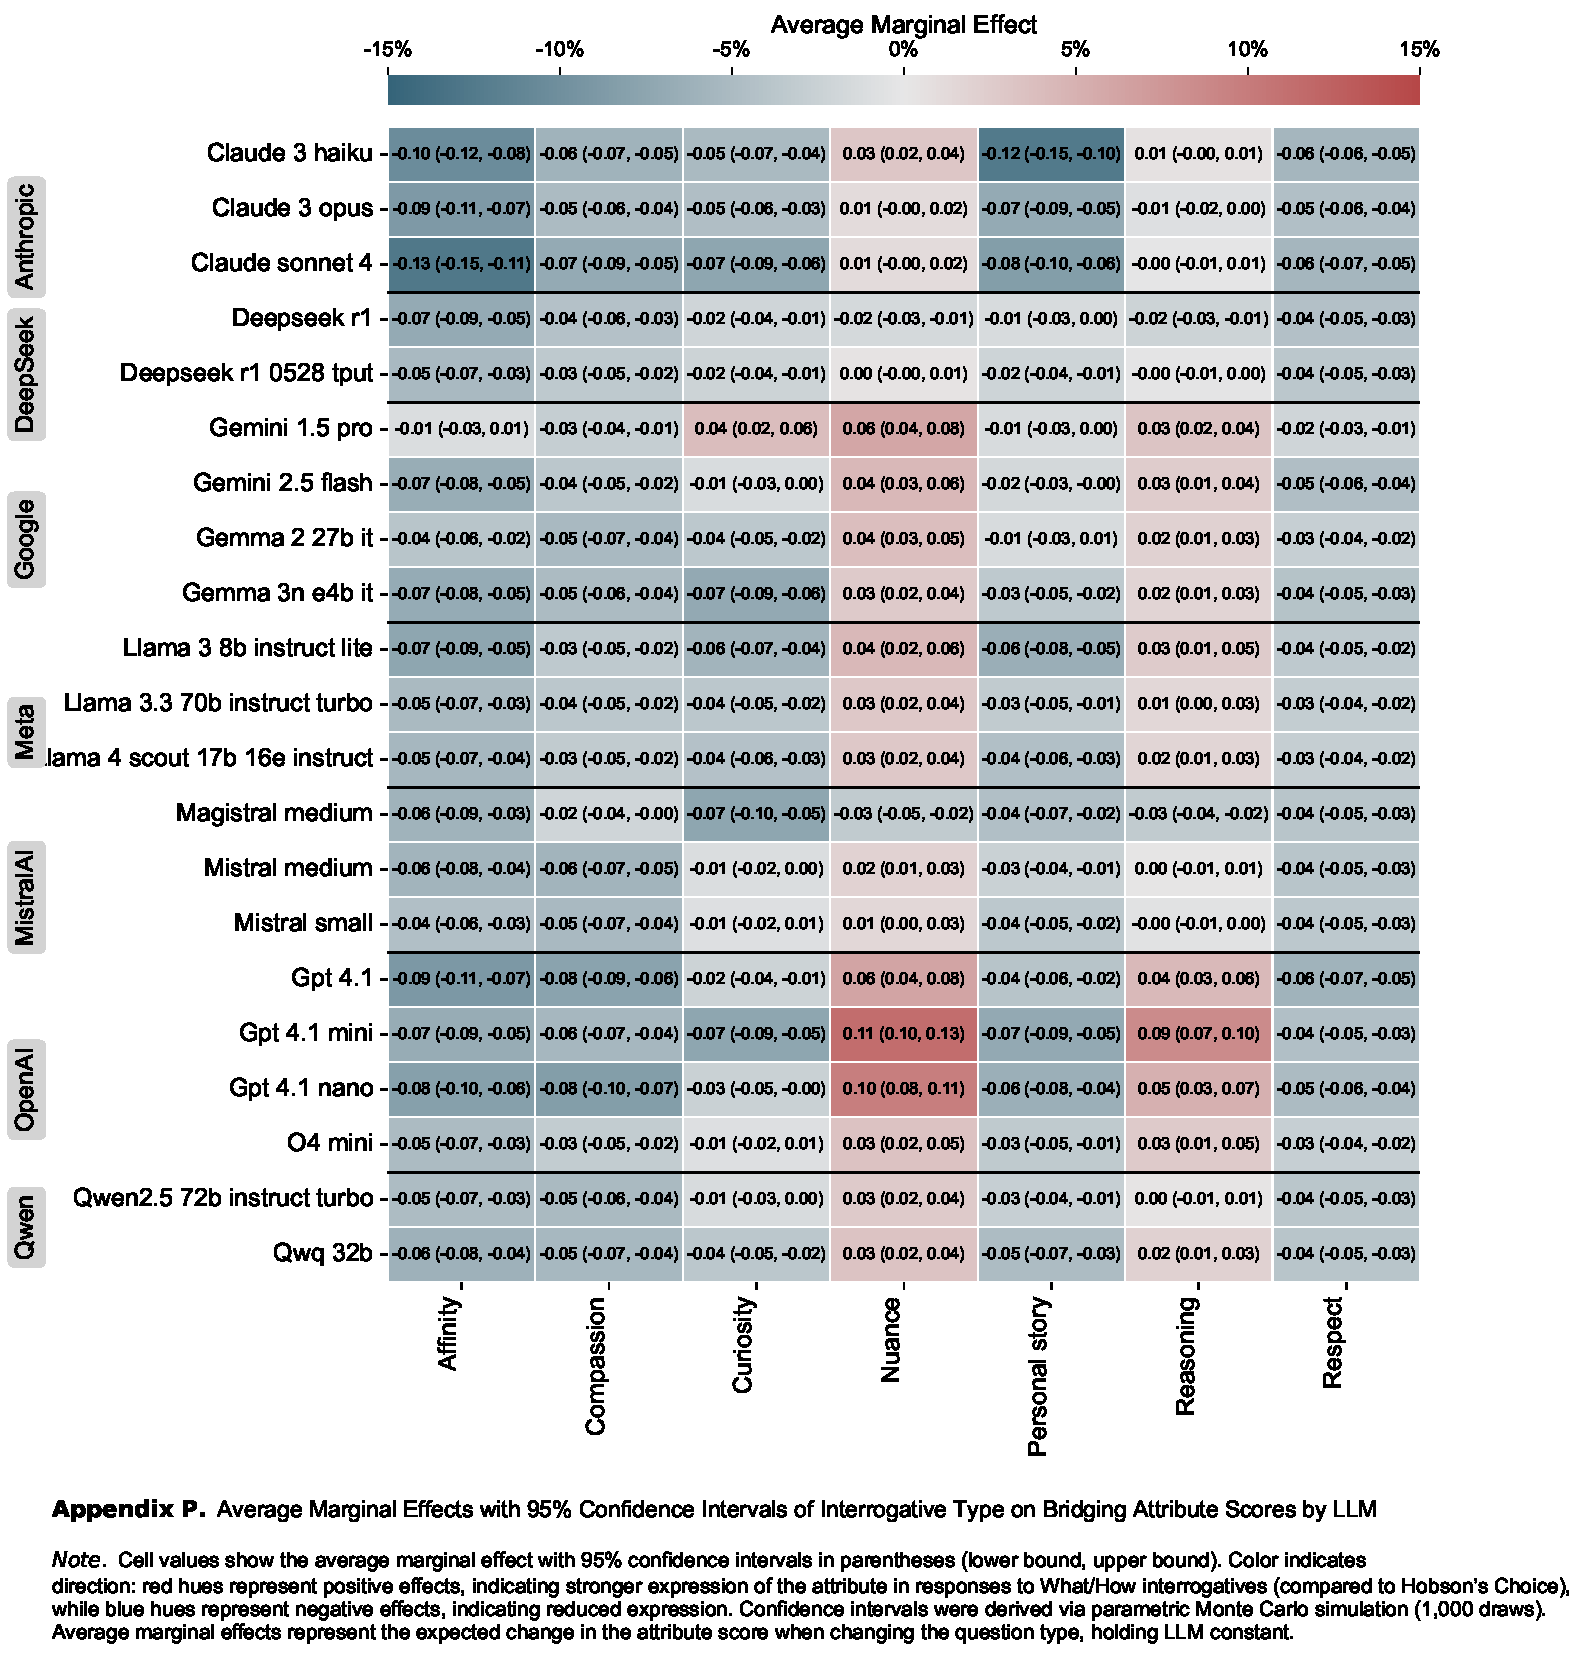
\includegraphics{../03_outputs/04_appendices/appendix_p} \end{center}

\clearpage

\section*{References}\label{references}
\addcontentsline{toc}{section}{References}

\phantomsection\label{refs}
\begin{CSLReferences}{1}{0}
\bibitem[\citeproctext]{ref-aoki_large_2024}
Aoki, G. (2024). \emph{Large {Language} {Models} in {Politics} and {Democracy}: {A} {Comprehensive} {Survey}}. arXiv. \url{https://doi.org/10.48550/arXiv.2412.04498}

\bibitem[\citeproctext]{ref-arelbundock_interpret_2024}
Arel-Bundock, V., Greifer, N., \& Heiss, A. (2024). How to interpret statistical models using {marginaleffects} for {R} and {Python}. \emph{Journal of Statistical Software}, \emph{111}(9), 1--32. \url{https://doi.org/10.18637/jss.v111.i09}

\bibitem[\citeproctext]{ref-barrie_replication_2025}
Barrie, C., Palmer, A., \& Spirling, A. (2025). \emph{Replication for {Language} {Models}}.

\bibitem[\citeproctext]{ref-belnap_logic_1976}
Belnap, N. D., \& Steel, T. B. (1976). \emph{The logic of questions and answers}. Yale University Press.

\bibitem[\citeproctext]{ref-bick_rapid_2024}
Bick, A., Blandin, A., \& Deming, D. J. (2024). \emph{The {Rapid} {Adoption} of {Generative} {AI}}. \url{https://doi.org/10.20955/wp.2024.027}

\bibitem[\citeproctext]{ref-bloom_taxonomy_1986}
Bloom, B. S. (1986). \emph{Taxonomy of educational objectives.} (29. print). Longman.

\bibitem[\citeproctext]{ref-brachman_current_2025}
Brachman, M., El-Ashry, A., Dugan, C., \& Geyer, W. (2025). \emph{Current and {Future} {Use} of {Large} {Language} {Models} for {Knowledge} {Work}}. arXiv. \url{https://doi.org/10.48550/arXiv.2503.16774}

\bibitem[\citeproctext]{ref-caluwaerts_deliberation_2023}
Caluwaerts, D., Bernaerts, K., Kesberg, R., Smets, L., \& Spruyt, B. (2023). Deliberation and polarization: A multi-disciplinary review. \emph{Frontiers in Political Science}, \emph{5}. \url{https://doi.org/10.3389/fpos.2023.1127372}

\bibitem[\citeproctext]{ref-chen_large_2025}
Chen, D., Parsa, R., Swanson, K., Nunez, J.-J., Critch, A., Bitterman, D. S., Liu, F.-F., \& Raman, S. (2025). Large language models in oncology: A review. \emph{BMJ Oncology}, \emph{4}(1), e000759. \url{https://doi.org/10.1136/bmjonc-2025-000759}

\bibitem[\citeproctext]{ref-chen_spiral_2024}
Chen, X., He, B., Lin, H., Han, X., Wang, T., Cao, B., Sun, L., \& Sun, Y. (2024). \emph{Spiral of {Silence}: {How} is {Large} {Language} {Model} {Killing} {Information} {Retrieval}? -- {A} {Case} {Study} on {Open} {Domain} {Question} {Answering}}. arXiv. \url{https://doi.org/10.48550/arXiv.2404.10496}

\bibitem[\citeproctext]{ref-devlin_bert_2018-1}
Devlin, J., Chang, M.-W., Lee, K., \& Toutanova, K. (2018). \emph{{BERT}: {Pre}-training of {Deep} {Bidirectional} {Transformers} for {Language} {Understanding}}. arXiv. \url{https://doi.org/10.48550/ARXIV.1810.04805}

\bibitem[\citeproctext]{ref-egami_using_2023}
Egami, N., Hinck, M., Stewart, B. M., \& Wei, H. (2023). \emph{Using {Imperfect} {Surrogates} for {Downstream} {Inference}: {Design}-based {Supervised} {Learning} for {Social} {Science} {Applications} of {Large} {Language} {Models}}. arXiv. \url{https://doi.org/10.48550/ARXIV.2306.04746}

\bibitem[\citeproctext]{ref-egami_dsl_2025}
Egami, N., Hinck, M., Stewart, B. M., \& Wei, H. (2025). \emph{Dsl: Design-based supervised learning}. \url{http://naokiegami.com/dsl/}

\bibitem[\citeproctext]{ref-elim_promoting_2024}
Elim, E. H. S. Y. (2024). Promoting cognitive skills in {AI}-supported learning environments: The integration of bloom's taxonomy. \emph{Education 3-13}, 1--11. \url{https://doi.org/10.1080/03004279.2024.2332469}

\bibitem[\citeproctext]{ref-gaber_evaluating_2025}
Gaber, F., Shaik, M., Allega, F., Bilecz, A. J., Busch, F., Goon, K., Franke, V., \& Akalin, A. (2025). Evaluating large language model workflows in clinical decision support for triage and referral and diagnosis. \emph{Npj Digital Medicine}, \emph{8}(1), 263. \url{https://doi.org/10.1038/s41746-025-01684-1}

\bibitem[\citeproctext]{ref-gal_dropout_2016}
Gal, Y., \& Ghahramani, Z. (2016). \emph{Dropout as a {Bayesian} {Approximation}: {Representing} {Model} {Uncertainty} in {Deep} {Learning}}. arXiv. \url{https://doi.org/10.48550/arXiv.1506.02142}

\bibitem[\citeproctext]{ref-gawlikowski_survey_2022}
Gawlikowski, J., Tassi, C. R. N., Ali, M., Lee, J., Humt, M., Feng, J., Kruspe, A., Triebel, R., Jung, P., Roscher, R., Shahzad, M., Yang, W., Bamler, R., \& Zhu, X. X. (2022). \emph{A {Survey} of {Uncertainty} in {Deep} {Neural} {Networks}}. arXiv. \url{https://doi.org/10.48550/arXiv.2107.03342}

\bibitem[\citeproctext]{ref-grice_studies_1991}
Grice, H. P. (1991). \emph{Studies in the way of words}. Harvard university press.

\bibitem[\citeproctext]{ref-guo_calibration_2017}
Guo, C., Pleiss, G., Sun, Y., \& Weinberger, K. Q. (2017). \emph{On {Calibration} of {Modern} {Neural} {Networks}}. arXiv. \url{https://doi.org/10.48550/arXiv.1706.04599}

\bibitem[\citeproctext]{ref-hakkarainen_interrogative_2002}
Hakkarainen, K., \& Sintonen, M. (2002). The {Interrogative} {Model} of {Inquiry} and {Computer}-{Supported} {Collaborative} {Learning}. \emph{Science and Education}, \emph{11}(1), 25--43. \url{https://doi.org/10.1023/a:1013076706416}

\bibitem[\citeproctext]{ref-huang_survey_2024}
Huang, H.-Y., Yang, Y., Zhang, Z., Lee, S., \& Wu, Y. (2024). \emph{A {Survey} of {Uncertainty} {Estimation} in {LLMs}: {Theory} {Meets} {Practice}}. arXiv. \url{https://doi.org/10.48550/arXiv.2410.15326}

\bibitem[\citeproctext]{ref-jiang_how_2020}
Jiang, Z., Xu, F. F., Araki, J., \& Neubig, G. (2020). How {Can} {We} {Know} {What} {Language} {Models} {Know}? \emph{Transactions of the Association for Computational Linguistics}, \emph{8}, 423--438. \url{https://doi.org/10.1162/tacl_a_00324}

\bibitem[\citeproctext]{ref-good_description_ddk_agb_2025}
Kadt, D. de, \& Grzymala-Busse, A. (2025). \emph{Good description}. \url{https://github.com/ddekadt/good_description/blob/main/good_description_ddk_agb.pdf}

\bibitem[\citeproctext]{ref-kasirzadeh_conversation_2023-1}
Kasirzadeh, A., \& Gabriel, I. (2023). In {Conversation} with {Artificial} {Intelligence}: {Aligning} language {Models} with {Human} {Values}. \emph{Philosophy \& Technology}, \emph{36}(2). \url{https://doi.org/10.1007/s13347-023-00606-x}

\bibitem[\citeproctext]{ref-kharchenko_how_2025}
Kharchenko, J., Roosta, T., Chadha, A., \& Shah, C. (2025). \emph{How {Well} {Do} {LLMs} {Represent} {Values} {Across} {Cultures}? {Empirical} {Analysis} of {LLM} {Responses} {Based} on {Hofstede} {Cultural} {Dimensions}}. arXiv. \url{https://doi.org/10.48550/arXiv.2406.14805}

\bibitem[\citeproctext]{ref-kim_applying_2025}
Kim, Y., Chin, B., Son, K., Kim, S., \& Kim, J. (2025). \emph{Applying the {Gricean} {Maxims} to a {Human}-{LLM} {Interaction} {Cycle}: {Design} {Insights} from a {Participatory} {Approach}}. arXiv. \url{https://doi.org/10.48550/ARXIV.2503.00858}

\bibitem[\citeproctext]{ref-kirk_prism_2024}
Kirk, H. R., Whitefield, A., Röttger, P., Bean, A., Margatina, K., Ciro, J., Mosquera, R., Bartolo, M., Williams, A., He, H., Vidgen, B., \& Hale, S. A. (2024). \emph{The {PRISM} {Alignment} {Dataset}: {What} {Participatory}, {Representative} and {Individualised} {Human} {Feedback} {Reveals} {About} the {Subjective} and {Multicultural} {Alignment} of {Large} {Language} {Models}}. \url{https://doi.org/10.48550/ARXIV.2404.16019}

\bibitem[\citeproctext]{ref-koralus_reason_2023}
Koralus, P. (2023). \emph{Reason and {Inquiry}: {The} {Erotetic} {Theory}}. Oxford University Press, Incorporated.

\bibitem[\citeproctext]{ref-koralus_pyetr_2025}
Koralus, P., Moss, S., \& Todd, M. (2025). \emph{{PyETR}}. University of Oxford; University of Birmingham; Dreaming Spires.

\bibitem[\citeproctext]{ref-krause_gricean_2024}
Krause, L., \& Vossen, P. T. J. M. (2024). The {Gricean} {Maxims} in {NLP} - {A} {Survey}. \emph{Proceedings of the 17th {International} {Natural} {Language} {Generation} {Conference}}, 470--485. \url{https://doi.org/10.18653/v1/2024.inlg-main.39}

\bibitem[\citeproctext]{ref-laux_improving_2023-1}
Laux, J., Stephany, F., \& Liefgreen, A. (2023). \emph{Improving {Task} {Instructions} for {Data} {Annotators}: {How} {Clear} {Rules} and {Higher} {Pay} {Increase} {Performance} in {Data} {Annotation} in the {AI} {Economy}}. arXiv. \url{https://doi.org/10.48550/ARXIV.2312.14565}

\bibitem[\citeproctext]{ref-lees_new_2022}
Lees, A., Tran, V. Q., Tay, Y., Sorensen, J., Gupta, J., Metzler, D., \& Vasserman, L. (2022). \emph{A {New} {Generation} of {Perspective} {API}: {Efficient} {Multilingual} {Character}-level {Transformers}}. arXiv. \url{https://doi.org/10.48550/arXiv.2202.11176}

\bibitem[\citeproctext]{ref-li_large_2023}
Li, C., Wang, J., Zhang, Y., Zhu, K., Hou, W., Lian, J., Luo, F., Yang, Q., \& Xie, X. (2023). \emph{Large {Language} {Models} {Understand} and {Can} be {Enhanced} by {Emotional} {Stimuli}}. arXiv. \url{https://doi.org/10.48550/arXiv.2307.11760}

\bibitem[\citeproctext]{ref-luo_enhanced_2025}
Luo, Y., Liu, T., Pang, P. C.-I., McKay, D., Chen, Z., Buchanan, G., \& Chang, S. (2025). \emph{Enhanced {Bloom}'s {Educational} {Taxonomy} for {Fostering} {Information} {Literacy} in the {Era} of {Large} {Language} {Models}}. arXiv. \url{https://doi.org/10.48550/ARXIV.2503.19434}

\bibitem[\citeproctext]{ref-massing_degrees_2017}
Massing, N., \& Schneider, S. L. (2017). Degrees of competency: The relationship between educational qualifications and adult skills across countries. \emph{Large-Scale Assessments in Education}, \emph{5}(1), 6. \url{https://doi.org/10.1186/s40536-017-0041-y}

\bibitem[\citeproctext]{ref-morucci_model_2024}
Morucci, M., \& Spirling, A. (2024). \emph{Model {Complexity} for {Supervised} {Learning}: {Why} {Simple} {Models} {Almost} {Always} {Work} {Best}, {And} {Why} {It} {Matters} for {Applied} {Research}}.

\bibitem[\citeproctext]{ref-novoa_generically_2023}
Novoa, G., Echelbarger, M., Gelman, A., \& Gelman, S. A. (2023). Generically partisan: {Polarization} in political communication. \emph{Proceedings of the National Academy of Sciences}, \emph{120}(47), e2309361120. \url{https://doi.org/10.1073/pnas.2309361120}

\bibitem[\citeproctext]{ref-ovadya_bridging_2023}
Ovadya, A., \& Thorburn, L. (2023). \emph{Bridging {Systems}: {Open} {Problems} for {Countering} {Destructive} {Divisiveness} across {Ranking}, {Recommenders}, and {Governance}}. arXiv. \url{https://doi.org/10.48550/arXiv.2301.09976}

\bibitem[\citeproctext]{ref-panzeri_childrens_2021}
Panzeri, F., \& Foppolo, F. (2021). Children's and adults' sensitivity to {Gricean} maxims and to the maximize presupposition principle. \emph{Frontiers in Psychology}, \emph{12}. \url{https://doi.org/10.3389/fpsyg.2021.624628}

\bibitem[\citeproctext]{ref-pavlovic_understanding_2025}
Pavlovic, M. (2025). \emph{Understanding {Model} {Calibration} -- {A} gentle introduction and visual exploration of calibration and the expected calibration error ({ECE})}. arXiv. \url{https://doi.org/10.48550/arXiv.2501.19047}

\bibitem[\citeproctext]{ref-pearl_understanding_2013}
Pearl, J. (2013). \emph{Understanding {Simpson}'s {Paradox}} {[}\{SSRN\} \{Scholarly\} \{Paper\}{]}. Social Science Research Network. \url{https://doi.org/10.2139/ssrn.2343788}

\bibitem[\citeproctext]{ref-pereira_language_2022}
Pereira, A., \& Ortiz, K. Z. (2022). Language skills differences between adults without formal education and low formal education. \emph{Psicologia: Reflexão e Crítica}, \emph{35}(1), 4. \url{https://doi.org/10.1186/s41155-021-00205-9}

\bibitem[\citeproctext]{ref-press_measuring_2023}
Press, O., Zhang, M., Min, S., Schmidt, L., Smith, N., \& Lewis, M. (2023). Measuring and {Narrowing} the {Compositionality} {Gap} in {Language} {Models}. In H. Bouamor, J. Pino, \& K. Bali (Eds.), \emph{Findings of the {Association} for {Computational} {Linguistics}: {EMNLP} 2023} (pp. 5687--5711). Association for Computational Linguistics. \url{https://doi.org/10.18653/v1/2023.findings-emnlp.378}

\bibitem[\citeproctext]{ref-razavi_benchmarking_2025}
Razavi, A., Soltangheis, M., Arabzadeh, N., Salamat, S., Zihayat, M., \& Bagheri, E. (2025). \emph{Benchmarking {Prompt} {Sensitivity} in {Large} {Language} {Models}}. arXiv. \url{https://doi.org/10.48550/arXiv.2502.06065}

\bibitem[\citeproctext]{ref-rottger_two_2022-1}
Röttger, P., Vidgen, B., Hovy, D., \& Pierrehumbert, J. (2022). Two {Contrasting} {Data} {Annotation} {Paradigms} for {Subjective} {NLP} {Tasks}. \emph{Proceedings of the 2022 {Conference} of the {North} {American} {Chapter} of the {Association} for {Computational} {Linguistics}: {Human} {Language} {Technologies}}. \url{https://doi.org/10.18653/v1/2022.naacl-main.13}

\bibitem[\citeproctext]{ref-saad_gricean_2025-1}
Saad, F., Murukannaiah, P. K., \& Singh, M. P. (2025). \emph{Gricean {Norms} as a {Basis} for {Effective} {Collaboration}}. arXiv. \url{https://doi.org/10.48550/ARXIV.2503.14484}

\bibitem[\citeproctext]{ref-schulhoff_prompt_2025}
Schulhoff, S., Ilie, M., Balepur, N., Kahadze, K., Liu, A., Si, C., Li, Y., Gupta, A., Han, H., Schulhoff, S., Dulepet, P. S., Vidyadhara, S., Ki, D., Agrawal, S., Pham, C., Kroiz, G., Li, F., Tao, H., Srivastava, A., \ldots{} Resnik, P. (2025). \emph{The {Prompt} {Report}: {A} {Systematic} {Survey} of {Prompt} {Engineering} {Techniques}}. arXiv. \url{https://doi.org/10.48550/arXiv.2406.06608}

\bibitem[\citeproctext]{ref-sclar_quantifying_2024}
Sclar, M., Choi, Y., Tsvetkov, Y., \& Suhr, A. (2024). \emph{Quantifying {Language} {Models}' {Sensitivity} to {Spurious} {Features} in {Prompt} {Design} or: {How} {I} learned to start worrying about prompt formatting}. arXiv. \url{https://doi.org/10.48550/arXiv.2310.11324}

\bibitem[\citeproctext]{ref-scorzato_reliability_2024}
Scorzato, L. (2024). Reliability and {Interpretability} in {Science} and {Deep} {Learning}. \emph{Minds and Machines}, \emph{34}(3), 27. \url{https://doi.org/10.1007/s11023-024-09682-0}

\bibitem[\citeproctext]{ref-shen_experimental_2023}
Shen, K., \& Kejriwal, M. (2023). An experimental study measuring the generalization of fine-tuned language representation models across commonsense reasoning benchmarks. \emph{Expert Systems}, \emph{40}(5), e13243. \url{https://doi.org/10.1111/exsy.13243}

\bibitem[\citeproctext]{ref-tamkin_understanding_2021}
Tamkin, A., Brundage, M., Clark, J., \& Ganguli, D. (2021). \emph{Understanding the {Capabilities}, {Limitations}, and {Societal} {Impact} of {Large} {Language} {Models}}. arXiv. \url{https://doi.org/10.48550/arXiv.2102.02503}

\bibitem[\citeproctext]{ref-thapa_large_2025}
Thapa, S., Shiwakoti, S., Shah, S. B., Adhikari, S., Veeramani, H., Nasim, M., \& Naseem, U. (2025). Large language models ({LLM}) in computational social science: Prospects, current state, and challenges. \emph{Social Network Analysis and Mining}, \emph{15}(1), 4. \url{https://doi.org/10.1007/s13278-025-01428-9}

\bibitem[\citeproctext]{ref-tran_investigation_2020}
Tran, T. T. H. T., Nguyen Thi Quynh Hoa. (2020). An investigation into the flouting of conversational maxims employed by male and female guests in the {American} talk show "{The} {Ellen} {Show}". \emph{Journal of Science and Technology Issue on Information and Communications Technology}, 117--122. \url{https://doi.org/10.31130/jst-ud2020-069e}

\bibitem[\citeproctext]{ref-de_vassimon_manela_stereotype_2021}
Vassimon Manela, D. de, Errington, D., Fisher, T., Breugel, B. van, \& Minervini, P. (2021). Stereotype and {Skew}: {Quantifying} {Gender} {Bias} in {Pre}-trained and {Fine}-tuned {Language} {Models}. In P. Merlo, J. Tiedemann, \& R. Tsarfaty (Eds.), \emph{Proceedings of the 16th {Conference} of the {European} {Chapter} of the {Association} for {Computational} {Linguistics}: {Main} {Volume}} (pp. 2232--2242). Association for Computational Linguistics. \url{https://doi.org/10.18653/v1/2021.eacl-main.190}

\bibitem[\citeproctext]{ref-viveros-munoz_does_2025}
Viveros-Muñoz, R., Carrasco-Sáez, J., Contreras-Saavedra, C., San-Martín-Quiroga, S., \& Contreras-Saavedra, C. E. (2025). Does the {Grammatical} {Structure} of {Prompts} {Influence} the {Responses} of {Generative} {Artificial} {Intelligence}? {An} {Exploratory} {Analysis} in {Spanish}. \emph{Applied Sciences}, \emph{15}(7), 3882. \url{https://doi.org/10.3390/app15073882}

\bibitem[\citeproctext]{ref-wang_aleatoric_2025}
Wang, T., Wang, Y., Zhou, J., Peng, B., Song, X., Zhang, C., Sun, X., Niu, Q., Liu, J., Chen, S., Chen, K., Li, M., Feng, P., Bi, Z., Liu, M., Zhang, Y., Fei, C., Yin, C. H., \& Yan, L. K. (2025). \emph{From {Aleatoric} to {Epistemic}: {Exploring} {Uncertainty} {Quantification} {Techniques} in {Artificial} {Intelligence}}. arXiv. \url{https://doi.org/10.48550/arXiv.2501.03282}

\bibitem[\citeproctext]{ref-weidinger_ethical_2021}
Weidinger, L., Mellor, J., Rauh, M., Griffin, C., Uesato, J., Huang, P.-S., Cheng, M., Glaese, M., Balle, B., Kasirzadeh, A., Kenton, Z., Brown, S., Hawkins, W., Stepleton, T., Biles, C., Birhane, A., Haas, J., Rimell, L., Hendricks, L. A., \ldots{} Gabriel, I. (2021). \emph{Ethical and social risks of harm from {Language} {Models}}. arXiv. \url{https://doi.org/10.48550/arXiv.2112.04359}

\bibitem[\citeproctext]{ref-yaacoub_assessing_2025}
Yaacoub, A., Da-Rugna, J., \& Assaghir, Z. (2025). \emph{Assessing {AI}-{Generated} {Questions}' {Alignment} with {Cognitive} {Frameworks} in {Educational} {Assessment}}. arXiv. \url{https://doi.org/10.48550/ARXIV.2504.14232}

\bibitem[\citeproctext]{ref-yin_should_2024}
Yin, Z., Wang, H., Horio, K., Kawahara, D., \& Sekine, S. (2024). \emph{Should {We} {Respect} {LLMs}? {A} {Cross}-{Lingual} {Study} on the {Influence} of {Prompt} {Politeness} on {LLM} {Performance}}. arXiv. \url{https://doi.org/10.48550/arXiv.2402.14531}

\bibitem[\citeproctext]{ref-zheng_grice_2021}
Zheng, Z., Qiu, S., Fan, L., Zhu, Y., \& Zhu, S.-C. (2021). {GRICE}: {A} {Grammar}-based {Dataset} for {Recovering} {Implicature} and {Conversational} {rEasoning}. In C. Zong, F. Xia, W. Li, \& R. Navigli (Eds.), \emph{Findings of the {Association} for {Computational} {Linguistics}: {ACL}-{IJCNLP} 2021} (pp. 2074--2085). Association for Computational Linguistics. \url{https://doi.org/10.18653/v1/2021.findings-acl.182}

\bibitem[\citeproctext]{ref-zhu_learn_2025}
Zhu, J., Kempermann, M., Cannanure, V. K., Hartland, A., Navarrete, R. M., Carteny, G., Braun, D., \& Weber, I. (2025). \emph{Learn, {Explore} and {Reflect} by {Chatting}: {Understanding} the {Value} of an {LLM}-{Based} {Voting} {Advice} {Application} {Chatbot}}. arXiv. \url{https://doi.org/10.48550/arXiv.2505.09806}

\end{CSLReferences}

\end{document}
